\documentclass[11pt,usletter]{report}
\usepackage{qmcpack_manual}
\usepackage{bibtopic}
\bibliographystyle{ieeetr}
\usepackage{amsmath}
\usepackage{amssymb}
\usepackage{delarray}
\usepackage{algorithmic}
\usepackage{algorithm}
\usepackage{makeidx}
\usepackage{fancyhdr}
\usepackage{hyperref} %for urls
\usepackage{tabularx}
\usepackage{placeins}
% environment for shaded verbatim
%\usepackage{verbatim}
\usepackage{caption}
\usepackage{graphicx}

% making listing behave properly
%   with setting below, listings now render correctly
%   copy/paste from pdf is still messed up (is this even possible to fix?)
%     -indentation whitespace is not preserved (needed for Python)
%     -copy/paste can result in mangled text
%     -mangling depends on pdf viewer (it is different for acroread and evince)
%     -verbatim suffers from this also

\usepackage{upquote}  % render ' properly
\usepackage{qmcpack_listings}

% set margins for whole document, lots of wasted space at top and bottom originally
\usepackage[left=1.0in,right=1.0in,top=1.0in,bottom=1.0in]{geometry}

\newcommand{\HRule}{\rule{\linewidth}{0.5mm}}
%% \newcommand{\courier}[1]{{\fontfamily{pcr}\selectfont #1}}

% for markup, as needed
\newcommand{\red}[1]{{\color{red} #1}}
\newcommand{\blue}[1]{{\color{blue} #1}}

% hide or show text relevant to developers
\newcommand{\dev}[1]{#1}
%\newcommand{\dev}[1]{}

% efficiently comment out/hide blocks of text for any purpose
\newcommand{\hide}[1]{}


% control display of instructions in the labs
%   normally one only wants to show the 'workstation' way of running the labs
\newif\ifws
\wstrue
%   for the pdf used during the labs, one wants to show the host supercomputer way
%\wsfalse
%  command for switching inline text (do not wrap verbatim environments with this!)
\ifws
\newcommand{\labsw}[2]{#1}
\else
\newcommand{\labsw}[2]{#2}
\fi


\oddsidemargin 0cm
\evensidemargin 0cm
\textwidth 6.5in


% proper rendering of qmcpack
\newcommand{\qmcpack}{{QMCPACK} } % apparently the trailing whitespace is significant

% mathematics convenience commands
\newcommand{\abs}[1]{\lvert #1 \rvert}
\newcommand{\norm}[1]{\lVert #1 \rVert}
\newcommand{\pnorm}[2]{\lVert #1 \rVert_{#2}}
\newcommand{\mean}[1]{\langle #1 \rangle}
\newcommand{\ket}[1]{\lvert #1 \rangle}
\newcommand{\bra}[1]{\langle #1 \rvert}
\newcommand{\expval}[3]{\bra{#1}#2\ket{#3}}
\newcommand{\expvalh}[3]{\bra{#1}\hat{#2}\ket{#3}}
\newcommand{\overlap}[2]{\langle #1 \lvert #2 \rangle}
\newcommand{\operator}[3]{\ket{#1} #2 \bra{#3}}
\newcommand{\idop}{\hat{\mathbb{1}}}
\newcommand{\bs}{\boldsymbol}
\newcommand{\tr}{\text{tr}} % trace


\begin{document}

\begin{btUnit}

\chapter{Lab 1: Monte Carlo Statistical Analysis}
\label{chap:lab_qmc_statistics}


\section{Topics covered in this Lab} 

This lab focuses on the basics of analyzing data from Monte Carlo (MC)
calculations.  In this lab, participants will use data from
VMC calculations of a simple one-electron system with an analytically soluble
system (the ground state of the hydrogen atom) to understand how to interpret a
MC situation.  Most of these analyses will also carry over to diffusion Monte
Carlo (DMC) simulations.  Topics covered include:
\begin{itemize}
  \item{averaging Monte Carlo variables}
  \item{the statisical error bar of mean values}
  \item{effects of autocorrelation and variance on the error bar}
  \item{the relationship between Monte Carlo timestep and autocorrelation}
  \item{the use of blocking to reduce autocorrelation}
  \item{the significance of the acceptance ratio}
  \item{the significance of the sample size}
  \item{how to determine whether a Monte Carlo run was successful}
  \item{the relationship between wavefunction quality and variance}
  \item{gauging the efficiency of Monte Carlo runs}
  \item{the cost of scaling up to larger system sizes}
\end{itemize}


\hide{
\subsection{How to get the most out of this lab}
Be sure to practice using the various flags in the qmca tool to analyze the
data.  Although some features are not yet implemented, this will get you used
to seeing how the values in the data files produce the averages, which are the
ultimate result of the MC simulations.
}

\section{Lab directories and files}

\footnotesize
\begin{verbatim}
labs/lab1_qmc_statistics/
│
├── atom                              - H atom VMC calculation
│   ├── H.s000.scalar.dat                - H atom VMC data 
│   └── H.xml                            - H atom VMC input file
│
├── autocorrelation                   - varying autocorrelation
│   ├── H.dat                            - data for gnuplot
│   ├── H.plt                            - gnuplot for time step vs. E_L, tau_c
│   ├── H.s000.scalar.dat                - H atom VMC data: time step = 10 
│   ├── H.s001.scalar.dat                - H atom VMC data: time step =  5 
│   ├── H.s002.scalar.dat                - H atom VMC data: time step =  2 
│   ├── H.s003.scalar.dat                - H atom VMC data: time step =  1 
│   ├── H.s004.scalar.dat                - H atom VMC data: time step =  0.5
│   ├── H.s005.scalar.dat                - H atom VMC data: time step =  0.2
│   ├── H.s006.scalar.dat                - H atom VMC data: time step =  0.1
│   ├── H.s007.scalar.dat                - H atom VMC data: time step =  0.05 
│   ├── H.s008.scalar.dat                - H atom VMC data: time step =  0.02
│   ├── H.s009.scalar.dat                - H atom VMC data: time step =  0.01
│   ├── H.s010.scalar.dat                - H atom VMC data: time step =  0.005
│   ├── H.s011.scalar.dat                - H atom VMC data: time step =  0.002
│   ├── H.s012.scalar.dat                - H atom VMC data: time step =  0.001
│   ├── H.s013.scalar.dat                - H atom VMC data: time step =  0.0005
│   ├── H.s014.scalar.dat                - H atom VMC data: time step =  0.0002
│   ├── H.s015.scalar.dat                - H atom VMC data: time step =  0.0001
│   └── H.xml                            - H atom VMC input file
│
├── average                            - Python scripts for average/std. dev.
│   ├── average.py                         - average five E_L from H atom VMC
│   ├── stddev2.py                         - standard deviation using (E_L)^2
│   └── stddev.py                          - standard deviation around the mean
│
├── basis                              - varying basis set for orbitals
│   ├── H__exact.s000.scalar.dat           - H atom VMC data using STO basis
│   ├── H_STO-2G.s000.scalar.dat           - H atom VMC data using STO-2G basis
│   ├── H_STO-3G.s000.scalar.dat           - H atom VMC data using STO-3G basis
│   └── H_STO-6G.s000.scalar.dat           - H atom VMC data using STO-6G basis
│
├── blocking                           - varying block/step ratio
│   ├── H.dat                              - data for gnuplot
│   ├── H.plt                              - gnuplot for N_block vs. E, tau_c
│   ├── H.s000.scalar.dat                  - H atom VMC data 50000:1 blocks:steps
│   ├── H.s001.scalar.dat                  - "  "    "    "  25000:2 blocks:steps
│   ├── H.s002.scalar.dat                  - "  "    "    "  12500:4 blocks:steps
│   ├── H.s003.scalar.dat                  - "  "    "    "  6250: 8 blocks:steps
│   ├── H.s004.scalar.dat                  - "  "    "    "  3125:16 blocks:steps
│   ├── H.s005.scalar.dat                  - "  "    "    "  2500:20 blocks:steps
│   ├── H.s006.scalar.dat                  - "  "    "    "  1250:40 blocks:steps
│   ├── H.s007.scalar.dat                  - "  "    "    "  1000:50 blocks:steps
│   ├── H.s008.scalar.dat                  - "  "    "    "  500:100 blocks:steps
│   ├── H.s009.scalar.dat                  - "  "    "    "  250:200 blocks:steps
│   ├── H.s010.scalar.dat                  - "  "    "    "  125:400 blocks:steps
│   ├── H.s011.scalar.dat                  - "  "    "    "  100:500 blocks:steps
│   ├── H.s012.scalar.dat                  - "  "    "    "  50:1000 blocks:steps
│   ├── H.s013.scalar.dat                  - "  "    "    "  40:1250 blocks:steps
│   ├── H.s014.scalar.dat                  - "  "    "    "  20:2500 blocks:steps
│   ├── H.s015.scalar.dat                  - "  "    "    "  10:5000 blocks:steps
│   └── H.xml                             - H atom VMC input file
│
├── blocks                             -  varying total number of blocks
│   ├── H.dat                             - data for gnuplot
│   ├── H.plt                             - gnuplot for N_block vs. E
│   ├── H.s000.scalar.dat                 - H atom VMC data    500 blocks
│   ├── H.s001.scalar.dat                 - "  "    "    "    2000 blocks
│   ├── H.s002.scalar.dat                 - "  "    "    "    8000 blocks
│   ├── H.s003.scalar.dat                 - "  "    "    "   32000 blocks
│   ├── H.s004.scalar.dat                 - "  "    "    "  128000 blocks
│   └── H.xml                             - H atom VMC input file 
│
├── dimer                          - comparing no and simple Jastrow factor
│   ├── H2_STO___no_jastrow.s000.scalar.dat - H dimer VMC data without Jastrow
│   └── H2_STO_with_jastrow.s000.scalar.dat - H dimer VMC data with Jastrow
│
├──  docs                               - documentation
│   ├──  Lab_1_MC_Analysis.pdf             - this document
│   └──  Lab_1_Slides.pdf                  - slides presented in the lab
│
├── nodes                              - varying number of computing nodes
│   ├──  H.dat                             - data for gnuplot
│   ├──  H.plt                             - gnuplot for N_node vs. E
│   ├──  H.s000.scalar.dat                 - H atom VMC data with  32 nodes
│   ├──  H.s001.scalar.dat                 - H atom VMC data with 128 nodes
│   └──  H.s002.scalar.dat                 - H atom VMC data with 512 nodes
│
├── problematic                        - problematic VMC run
│   └──  H.s000.scalar.dat                 - H atom VMC data with a problem
│
└── size                                - scaling with number of particles
    ├──  01________H.s000.scalar.dat       - H atom VMC data
    ├──  02_______H2.s000.scalar.dat       - H dimer "   "
    ├──  06________C.s000.scalar.dat       - C atom  "   "
    ├──  10______CH4.s000.scalar.dat       - methane "   "
    ├──  12_______C2.s000.scalar.dat       - C dimer "   "
    ├──  16_____C2H4.s000.scalar.dat       - ethene  " 
    ├──  18___CH4CH4.s000.scalar.dat       - methane dimer VMC data
    ├──  32_C2H4C2H4.s000.scalar.dat       - ethene dimer   "   "
    ├──  nelectron_tcpu.dat                - data for gnuplot
    └──  Nelectron_tCPU.plt                - gnuplot for N_elec vs. t_CPU
\end{verbatim}
\normalsize

\section{Atomic units} 

QMCPACK operates in Hartree atomic units to reduce the
number of factors in the Schr\"odinger equation.  Thus, the unit of length is
the bohr (5.291772 $\times 10^{-11}$ m = 0.529177 \AA); the unit of energy is
the hartree (4.359744 $\times 10^{-18}$ J = 27.211385 eV).  The energy of the
ground state of the hydrogen atom in these units is -0.5 hartrees.


%\section{Monte Carlo data analysis:\newline average, error bars, variance}

\section{Reviewing statistics}
\label{sec:review}

We will practice taking the average (mean) and standard deviation of some Monte
Carlo data by hand to review the basic definitions.

Enter Python's command line by typing \textbf{python [Enter]}.
You will see a prompt ``\textgreater\textgreater\textgreater''.

The mean of a data set is given by:
\begin{align}
  \overline{x} = \frac{1}{N}\sum_{i=1}^{N} x_i
\end{align}

To calculate the average of five local energies from a MC calculation of the
ground state of an electron in the hydrogen atom, input (truncate at the
thousandths place if you cannot copy and paste; script versions are also
available in the \texttt{average} directory): 

\begin{lstlisting}[style=SHELL]
(
(-0.45298911858) + 
(-0.45481953564) + 
(-0.48066105923) + 
(-0.47316713469) + 
(-0.46204733302)
)/5.
\end{lstlisting} 

Then, press \textbf{[Enter]} to get:

\begin{shade}
>>> ((-0.45298911858) + (-0.45481953564) + (-0.48066105923) + 
(-0.47316713469) + (-0.4620473302))/5.  
-0.46473683566800006
\end{shade}

To understand the significance of the mean, we also need the standard deviation
around the mean of the data (also called the error bar), given by:

\begin{align}
  \sigma = \sqrt{\frac{1}{N(N-1)}\sum_{i=1}^{N} ({x_i} - \overline{x})^2}
\end{align}

To calculate the standard deviation around the mean (-0.464736835668) of these
five data points, put in: 

\begin{lstlisting}[style=SHELL]
( (1./(5.*(5.-1.))) * ( 
(-0.45298911858-(-0.464736835668))**2 + \\
(-0.45481953564-(-0.464736835668))**2 + 
(-0.48066105923-(-0.464736835668))**2 + 
(-0.47316713469-(-0.464736835668))**2 + 
(-0.46204733302-(-0.464736835668))**2 ) 
)**0.5
\end{lstlisting} 

Then, press \textbf{[Enter]} to get:

\begin{shade}
>>> ( (1./(5.*(5.-1.))) * ( (-0.45298911858-(-0.464736835668))**2 +
(-0.45481953564-(-0.464736835668))**2 + (-0.48066105923-(-0.464736835668))**2 + 
(-0.47316713469-(-0.464736835668))**2 + (-0.46204733302-(-0.464736835668))**2 
) )**0.5
0.0053303187464332066
\end{shade}

Thus, we might report this data as having a value -0.465 +/- 0.005 hartrees.
This calculation of the standard deviation assumes that the average for this
data is fixed, but we may continually add Monte Carlo samples to the data so it
is better to use an estimate of the error bar that does not rely on the overall
average.  Such an estimate is given by:

\begin{align}
  \tilde{\sigma} = \sqrt{\frac{1}{N-1}\sum_{i=1}^{N} \left[{(x^2)}_i - ({x_i})^2\right]}
\end{align}

To calculate the standard deviation with this formula, input the following,
which includes the square of the local energy calculated with each
corresponding local energy:

\begin{lstlisting}[style=SHELL]
( (1./(5.-1.)) * ( 
(0.60984565298-(-0.45298911858)**2) + \\
(0.61641291630-(-0.45481953564)**2) + 
(1.35860151160-(-0.48066105923)**2) + \\
(0.78720769003-(-0.47316713469)**2) + 
(0.56393677687-(-0.46204733302)**2) ) 
)**0.5
\end{lstlisting}

and press \textbf{[Enter]} to get:

\begin{shade}
>>> ((1./(5.-1.))*((0.60984565298-(-0.45298911858)**2)+ 
(0.61641291630-(-0.45481953564)**2)+(1.35860151160-(-0.48066105923)**2)+ 
(0.78720769003-(-0.47316713469)**2)+(0.56393677687-(-0.46204733302)**2))
)**0.5
0.84491636672906634
\end{shade}

This much larger standard deviation, acknowledging that the mean of this small
data set is not the average in the limit of infinite sampling more accurately,
reports the value of the local energy as -0.5 +/- 0.8 hartrees.

Type \textbf{quit()} and press \textbf{[Enter]} to exit the Python command line.

\section{Inspecting Monte Carlo data}
\label{sec:inspect_data} 

QMCPACK outputs data from MC calculations into files ending in scalar.dat.
Several quantities are calculated and written for each block of Monte Carlo
steps in successive columns to the right of the step index. 

Change directories to \texttt{atom}, and open the file ending in
scalar.dat with a text editor (e.g., \textbf{vi *.scalar.dat} or \textbf{emacs
*.scalar.dat}.  If possible, adjust the terminal so that lines do not wrap.
The data will begin as follows (broken into three groups to fit on this page):

\begin{shade}
#   index    LocalEnergy         LocalEnergy_sq      LocalPotential     ...
         0   -4.5298911858e-01    6.0984565298e-01   -1.1708693521e+00    
         1   -4.5481953564e-01    6.1641291630e-01   -1.1863425644e+00    
         2   -4.8066105923e-01    1.3586015116e+00   -1.1766446209e+00    
         3   -4.7316713469e-01    7.8720769003e-01   -1.1799481122e+00    
         4   -4.6204733302e-01    5.6393677687e-01   -1.1619244081e+00    
         5   -4.4313854290e-01    6.0831516179e-01   -1.2064503041e+00    
         6   -4.5064926960e-01    5.9891422196e-01   -1.1521370176e+00    
         7   -4.5687452611e-01    5.8139614676e-01   -1.1423627617e+00    
         8   -4.5018503739e-01    8.4147849706e-01   -1.1842075439e+00    
         9   -4.3862013841e-01    5.5477715836e-01   -1.2080979177e+00    
\end{shade}

The first line begins with a \#, indicating that this line does not contain MC
data but rather the labels of the columns.  After a blank line, the remaining
lines consist of the MC data.  The first column, labeled index, is an integer
indicating which block of MC data is on that line.  The second column contains
the quantity usually of greatest interest from the simulation, the local
energy.  Since this simulation did not use the exact ground state wave
function, it does not produce -0.5 hartrees as the local energy although the
value lies within about 10\%.  The value of the local energy fluctuates from
block to block and the closer the trial wave function is to the ground state,
the smaller these fluctuations will be.  The next column contains an important
ingredient in estimating the error in the MC average--the square of the local
energy--found by evaluating the square of the Hamiltonian.  

\begin{shade} 
...   Kinetic             Coulomb             BlockWeight        ... 
       7.1788023352e-01   -1.1708693521e+00    1.2800000000e+04   
       7.3152302871e-01   -1.1863425644e+00    1.2800000000e+04   
       6.9598356165e-01   -1.1766446209e+00    1.2800000000e+04   
       7.0678097751e-01   -1.1799481122e+00    1.2800000000e+04   
       6.9987707508e-01   -1.1619244081e+00    1.2800000000e+04   
       7.6331176120e-01   -1.2064503041e+00    1.2800000000e+04   
       7.0148774798e-01   -1.1521370176e+00    1.2800000000e+04   
       6.8548823555e-01   -1.1423627617e+00    1.2800000000e+04   
       7.3402250655e-01   -1.1842075439e+00    1.2800000000e+04   
       7.6947777925e-01   -1.2080979177e+00    1.2800000000e+04   
\end{shade}

The fourth column from the left consists of the values of the local potential
energy.  In this simulation, it is identical to the Coulomb potential
(contained in the sixth column) because the one electron in the simulation has
only the potential energy coming from its interaction with the nucleus.  In
many-electron simulations, the local potential energy contains contributions
from the electron-electron Coulomb interactions and the nuclear potential or
pseudopotential.  The fifth column contains the local kinetic energy value for
each MC block, obtained from the Laplacian of the wave function.  The sixth
column shows the local Coulomb interaction energy.  The seventh column displays
the weight each line of data has in the average (the weights are identical in
this simulation).   

\begin{shade} 
...    BlockCPU            AcceptRatio         
       6.0178991748e-03    9.8515625000e-01
       5.8323097461e-03    9.8562500000e-01
       5.8213412744e-03    9.8531250000e-01
       5.8330412549e-03    9.8828125000e-01
       5.8108362256e-03    9.8625000000e-01
       5.8254170264e-03    9.8625000000e-01
       5.8314813086e-03    9.8679687500e-01
       5.8258469971e-03    9.8726562500e-01
       5.8158433545e-03    9.8468750000e-01
       5.7959401123e-03    9.8539062500e-01
\end{shade}

The eighth column shows the CPU time (in seconds) to calculate the data in that
line.  The ninth column from the left contains the acceptance ratio (1 being
full acceptance) for Monte Carlo steps in that line's data.  Other than the
block weight, all quantities vary from line to line.

Exit the text editor (\textbf{[Esc] :q! [Enter]} in vi, \textbf{[Ctrl]-x [Ctrl]-c} in
emacs).

\section{Averaging quantities in the MC data}
\label{sec:averaging} 

QMCPACK includes the qmca Python tool to average quantities in the scalar.dat file (and
also the dmc.dat file of DMC simulations).  Without any flags, qmca will output
the average of each column with a quantity in the scalar.dat file as follows. 

Execute qmca by \textbf{qmca *.scalar.dat}, which for this data outputs:

\begin{shade}

H  series 0 
LocalEnergy           =          -0.45446 +/-          0.00057
Variance              =             0.529 +/-            0.018 
Kinetic               =            0.7366 +/-           0.0020
LocalPotential        =           -1.1910 +/-           0.0016
Coulomb               =           -1.1910 +/-           0.0016 
LocalEnergy_sq        =             0.736 +/-            0.018
BlockWeight           =    12800.00000000 +/-       0.00000000
BlockCPU              =        0.00582002 +/-       0.00000067 
AcceptRatio           =          0.985508 +/-         0.000048
Efficiency            =        0.00000000 +/-       0.00000000 
\end{shade}

After one blank, qmca prints the title of the subsequent data, gleaned from the
data file name.  In this case, H.s000.scalar.dat became ``H  series 0''.
Everything before the first ``.s'' will be interpreted as the title, and the
number between ``.s'' and the next ``.'' will be interpreted as the series
number. 

The first column under the title is the name of each quantity qmca averaged.
The column to the right of the equal signs contains the average for the
quantity of that line, and the column to the right of the plus-slash-minus is
the statistical error bar on the quantity.  All quantities calculated from MC
simulations have and must be reported with a statistical error bar!

Two new quantities not present in the scalar.dat file are computed by qmca from
the data--variance and efficiency.  We will look at these later in this lab. 

To view only one value, \textbf{qmca} takes the \textbf{-q (quantity)} flag.
For example, the output of \textbf{qmca -q LocalEnergy *.scalar.dat} in this
directory produces a single line of output:

\begin{shade} 
H  series 0  LocalEnergy = -0.454460 +/- 0.000568 
\end{shade}

Type \textbf{qmca --help} to see the list of all quantities and their
abbreviations.

\section{Evaluating MC simulation quality}

There are several aspects of a MC simulation to consider in deciding how well
it went.  Besides the deviation of the average from an expected value (if there
is one), the stability of the simulation in its sampling, the autocorrelation
between MC steps, the value of the acceptance ratio (accepted steps over total
proposed steps), and the variance in the local energy all indicate the quality
of a MC simulation.  We will look at these one by one.

\subsection{Tracing MC quantities}

Visualizing the evolution of MC quantities over the course of the simulation by
a \textit{trace} offers a quick picture of whether the random walk had expected
behavior.  qmca plots traces with the -t flag.

Type \textbf{qmca -q e -t H.s000.scalar.dat}, which produces a graph of the
trace of the local energy:

\FloatBarrier
\begin{figure}[ht!]
\begin{center}
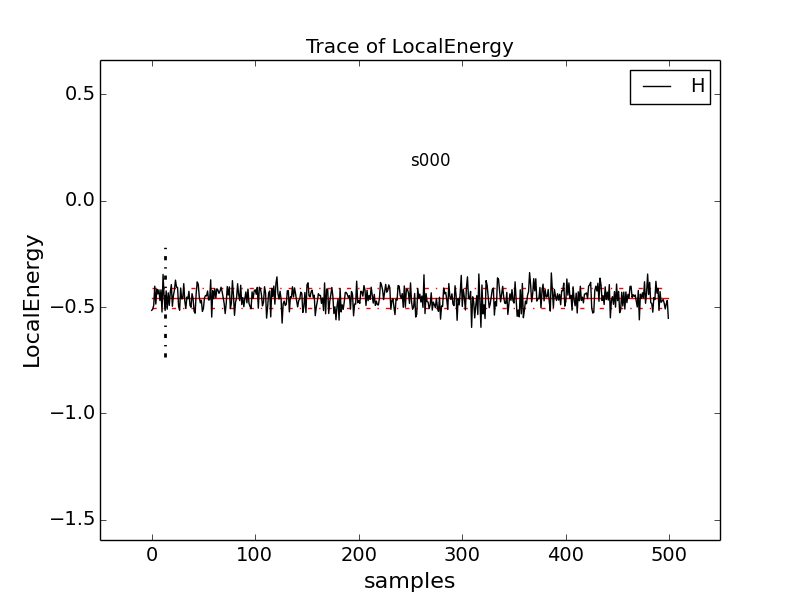
\includegraphics[trim = 0mm 0mm 0mm 0mm, clip,width=0.75\columnwidth]{./figures/lab_qmc_statistics_tracing1.png}
\end{center}
\end{figure}
\FloatBarrier

%\includegraphics[scale=0.5]{E_L_H_STO-2G.png}

The solid black line connects the values of the local energy at each MC block
(labeled ``samples'').  The average value is marked with a horizontal, solid
red line.  One standard deviation above and below the average are marked with
horizontal, dashed red lines.  

The trace of this run is largely centered around the average with no
large-scale oscillations or major shifts, indicating a good quality MC run. 

Try tracing the kinetic and potential energies, seeing that their behavior is
comparable to the total local energy.

Change to directory \texttt{problematic} and type \textbf{qmca -q e -t
H.s000.scalar.dat} to produce this graph:

\FloatBarrier
\begin{figure}[ht!]
\begin{center}
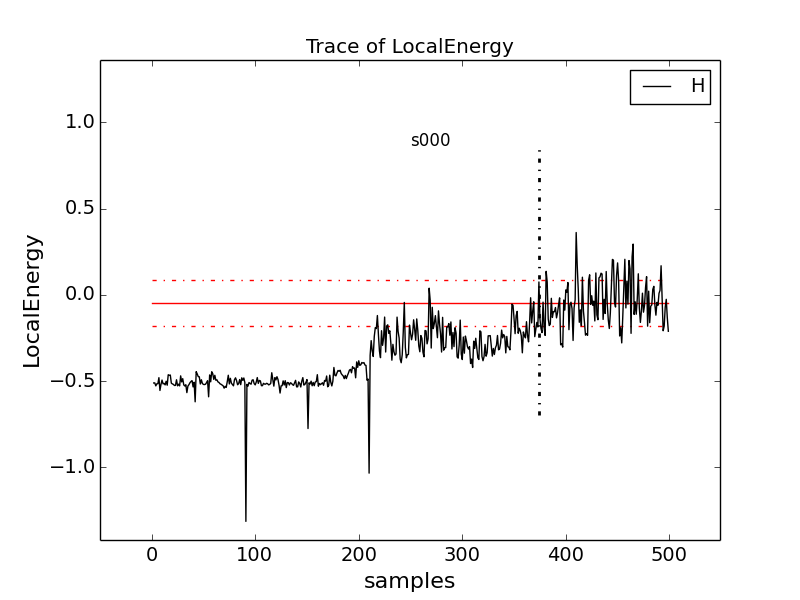
\includegraphics[trim = 0mm 0mm 0mm 0mm, clip,width=0.75\columnwidth]{./figures/lab_qmc_statistics_tracing2.png}
\end{center}
\end{figure}
\FloatBarrier

%\includegraphics[scale=0.5]{E_L_H_B-splines.png}

Here, the local energy samples cluster around the expected -0.5 hartrees for the
first 150 samples or so and then begin to oscillate more wildly and increase
erratically toward 0, indicating a poor quality MC run.

Again, trace the kinetic and potential energies in this run and see how their
behavior compares to the total local energy.

\subsection{Blocking away autocorrelation}

\textit{Autocorrelation} occurs when a given MC step biases subsequent MC
steps, leading to samples that are not statistically independent.  We must take
this autocorrelation into account in order to obtain accurate statistics.  qmca
outputs autocorrelation when given the {-}{-}sac flag.

Change to directory \texttt{autocorrelation} and type \textbf{qmca -q e
{-}{-}sac H.s000.scalar.dat}.  

\begin{shade} 
H  series 0  LocalEnergy = -0.454982 +/- 0.000430    1.0 
\end{shade}

The value after the error bar on the quantity is the autocorrelation (1.0 in
this case).

Proposing too small a step in configuration space, the MC \textit{time step},
can lead to autocorrelation since the new samples will be in the neighborhood
of previous samples.  Type \textbf{grep timestep H.xml} to see the varying time
step values in this QMCPACK input file (H.xml):

\begin{shade} 
<parameter name="timestep">10</parameter>
<parameter name="timestep">5</parameter> 
<parameter name="timestep">2</parameter> 
<parameter name="timestep">1</parameter>
<parameter name="timestep">0.5</parameter> 
<parameter name="timestep">0.2</parameter> 
<parameter name="timestep">0.1</parameter>
<parameter name="timestep">0.05</parameter> 
<parameter name="timestep">0.02</parameter> 
<parameter name="timestep">0.01</parameter>
<parameter name="timestep">0.005</parameter> 
<parameter name="timestep">0.002</parameter> 
<parameter name="timestep">0.001</parameter>
<parameter name="timestep">0.0005</parameter> 
<parameter name="timestep">0.0002</parameter> 
<parameter name="timestep">0.0001</parameter> 
\end{shade}

Generally, as the time step decreases, the autocorrelation will increase
(caveat: very large time steps will also have increasing autocorrelation). To
see this, type \textbf{qmca -q e {-}{-}sac *.scalar.dat} to see the energies
and autocorrelation times, then plot with gnuplot by inputting \textbf{gnuplot
H.plt}:

\FloatBarrier
\begin{figure}[ht!]
\begin{center}
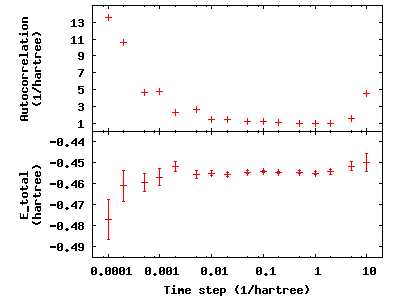
\includegraphics[trim = 0mm 0mm 0mm 0mm, clip,width=0.75\columnwidth]{./figures/lab_qmc_statistics_blocking1.png}
\end{center}
\end{figure}
\FloatBarrier

%\includegraphics[scale=1.0]{timestep_vs_autocorrelation_energy_H_STO-2G.png}

The error bar also increases with the autocorrelation.  

Press \textbf{q [Enter]} to quit gnuplot.

To get around the bias of autocorrelation, we group the MC steps into blocks,
take the average of the data in the steps of each block, and then finally
average the averages in all the blocks.  QMCPACK outputs the block averages as
each line in the scalar.dat file.  (For DMC simulations, in addition to the
scalar.dat, QMCPACK outputs the quantities at each step to the dmc.dat file,
which permits reblocking the data differently from the specification in the
input file.) 

Change directories to \texttt{blocking}.  Here we look at the time step of the
last data set in the \texttt{autocorrelation} directory.  Verify this by typing
\textbf{grep timestep H.xml} to see that all values are set to 0.001.  Now to
see how we will vary the blocking, type \textbf{grep -A1 blocks H.xml}.  The
parameter ``steps'' indicates the number of steps per block, and the parameter
``blocks'' gives the number of blocks.  For this comparison, the total number
of MC steps (equal to the product of ``steps'' and ``blocks'') is fixed at
50000.  Now check the effect of blocking on autocorrelation--type \textbf{qmca
-q e {-}{-}sac *scalar.dat} to see the data and \textbf{gnuplot H.plt} to
visualize the data:

%\begin{shaded} 
%\begin{verbatim} 
%H  series 0  LocalEnergy = -0.454433 +/- 0.003970   189.2 
%H  series 1  LocalEnergy = -0.453352 +/- 0.004159   104.5 
%H  series 2  LocalEnergy = -0.449211 +/- 0.006544   114.1 
%H  series 3  LocalEnergy = -0.449491 +/- 0.014770   381.1 
%H  series 4  LocalEnergy = -0.446602 +/- 0.008809   78.2 
%H  series 5  LocalEnergy = -0.488471 +/- 0.006704   27.2 
%H  series 6  LocalEnergy = -0.427345 +/- 0.011377   50.0 
%H  series 7  LocalEnergy = -0.456044 +/- 0.014513   51.1 
%H  series 8  LocalEnergy = -0.453782 +/- 0.016594   24.1 
%H  series 9  LocalEnergy = -0.482306 +/- 0.028252   21.6 
%H  series 10  LocalEnergy = -0.405258 +/- 0.013696   22.4 
%H  series 11  LocalEnergy = -0.423111 +/- 0.003579    2.9 
%H  series 12  LocalEnergy = -0.474759 +/- 0.016879    9.6 
%H  series 13  LocalEnergy = -0.414045 +/- 0.003606    5.5 
%H  series 14  LocalEnergy = -0.432808 +/- 0.004773    3.3 
%H  series 15  LocalEnergy = -0.465723 +/- 0.004425    2.6 
%\end{verbatim}
%\end{shaded}

\FloatBarrier
\begin{figure}[ht!]
\begin{center}
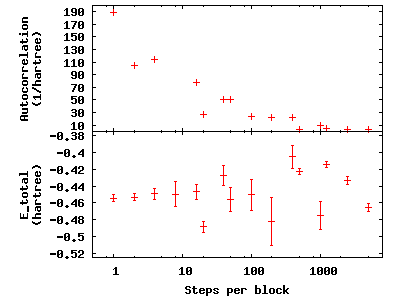
\includegraphics[trim = 0mm 0mm 0mm 0mm, clip,width=0.75\columnwidth]{./figures/lab_qmc_statistics_blocking2.png}
\end{center}
\end{figure}
\FloatBarrier

%\includegraphics[scale=1.0]{steps_per_block_vs_autocorrelation_energy_H_STO-2G.png}

The greatest number of steps per block produces the smallest autocorrelation
time.  The larger number of blocks over which to average at small
step-per-block number masks the corresponding increase in error bar with
increasing autocorrelation.

Press \textbf{q [Enter]} to quit gnuplot.

\subsection{Balancing autocorrelation and acceptance ratio}

Adjusting the time step value also affects the ratio of accepted steps to
proposed steps.  Stepping nearby in configuration space implies that the
probability distribution is similar and thus more likely to result in an
accepted move.  Keeping the acceptance ratio high means the algorithm is
efficiently exploring configuration space and not sticking at particular
configurations.  Return to the \ishell{autocorrelation} directory.  Refresh your
memory on the time steps in this set of simulations by \textbf{grep timestep
H.xml}. Then, type \textbf{qmca -q ar *scalar.dat} to see the acceptance ratio
as it varies with decreasing time step:

\begin{shade} 
H  series 0  AcceptRatio = 0.047646 +/- 0.000206 
H  series 1  AcceptRatio = 0.125361 +/- 0.000308 
H  series 2  AcceptRatio = 0.328590 +/- 0.000340 
H  series 3  AcceptRatio = 0.535708 +/- 0.000313 
H  series 4  AcceptRatio = 0.732537 +/- 0.000234 
H  series 5  AcceptRatio = 0.903498 +/- 0.000156 
H  series 6  AcceptRatio = 0.961506 +/- 0.000083 
H  series 7  AcceptRatio = 0.985499 +/- 0.000051 
H  series 8  AcceptRatio = 0.996251 +/- 0.000025 
H  series 9  AcceptRatio = 0.998638 +/- 0.000014 
H  series 10  AcceptRatio = 0.999515 +/- 0.000009 
H  series 11  AcceptRatio = 0.999884 +/- 0.000004 
H  series 12  AcceptRatio = 0.999958 +/- 0.000003 
H  series 13  AcceptRatio = 0.999986 +/- 0.000002 
H  series 14  AcceptRatio = 0.999995 +/- 0.000001 
H  series 15  AcceptRatio = 0.999999 +/- 0.000000 
\end{shade}

By series 8 (time step = 0.02), the acceptance ratio is in excess of 99\%.  

Considering the increase in autocorrelation and subsequent increase in error
bar as time step decreases, it is important to choose a time step that trades
off appropriately between acceptance ratio and autocorrelation.  In this
example, a time step of 0.02 occupies a spot where acceptance ratio is high
(99.6\%), and autocorrelation is not appreciably larger than the minimum value
(1.4 vs. 1.0).

\subsection{Considering variance}

Besides autocorrelation, the dominant contributor to the error bar is the
\textit{variance} in the local energy.  The variance measures the fluctuations
around the average local energy, and, as the fluctuations go to zero, the wave
function reaches an exact eigenstate of the Hamiltonian.  qmca calculates this
from the local energy and local energy squared columns of the scalar.dat. 

Type \textbf{qmca -q v H.s009.scalar.dat} to calculate the variance on the run
with time step balancing autocorrelation and acceptance ratio:

\begin{shade}
H  series 9  Variance = 0.513570 +/- 0.010589  
\end{shade}

Just as the total energy doesn't tell us much by itself, neither does the
variance.  However, comparing the ratio of the variance to the energy indicates
how the magnitude of the fluctuations compares to the energy itself.   Type
\textbf{qmca -q ev H.s009.scalar.dat} to calculate the energy and variance on
the run side by side with the ratio:

\begin{shade}
                     LocalEnergy               Variance        ratio
H  series 0  -0.454460 +/- 0.000568   0.529496 +/- 0.018445   1.1651
\end{shade}

1.1651 is a very high ratio indicating the square of the fluctuations is on
average larger than the value itself.  In the next section, we will approach
ways to improve the variance that subsequent labs will build upon.  

\section{Reducing statistical error bars}

\subsection{Increasing MC sampling}

Increasing the number of MC samples in a data set reduces the error bar as the
inverse of the square root of the number of samples.  There are two ways to
increase the number of MC samples in a simulation: running more samples in
parallel and increasing the number of blocks (with fixed number of steps per
block, this increases the total number of MC steps).

To see the effect of the running more samples in parallel, change to the
directory \ishell{nodes}.  The series here increases the number of nodes by
factors of four from 32 to 128 to 512.  Type \textbf{qmca -q ev *scalar.dat}
and note the change in the error bar on the local energy as the number of
nodes.  Visualize this with \textbf{gnuplot H.plt}:

\FloatBarrier
\begin{figure}[ht!]
\begin{center}
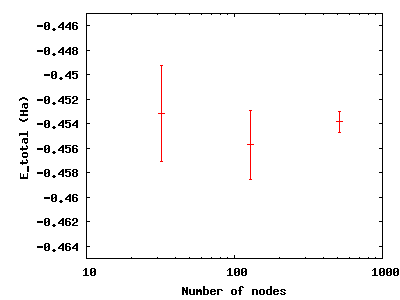
\includegraphics[trim = 0mm 0mm 0mm 0mm, clip,width=0.75\columnwidth]{./figures/lab_qmc_statistics_nodes.png}
\end{center}
\end{figure}
\FloatBarrier

%\includegraphics[scale=1.0]{nnode_vs_energy_H_STO-2G.png}

Increasing the number of blocks, unlike running in parallel, increases the
total CPU time of the simulation.  

Press \textbf{q [Enter]} to quit gnuplot.

To see the effect of increasing the block number, change to the directory
\ishell{blocks}. To see how we will vary the number of blocks, type
\textbf{grep -A1 blocks H.xml}.  The number of steps remains fixed, thus
increasing the total number of samples.   Visualize the tradeoff by inputting
\textbf{gnuplot H.plt}: 

\FloatBarrier
\begin{figure}[ht!]
\begin{center}
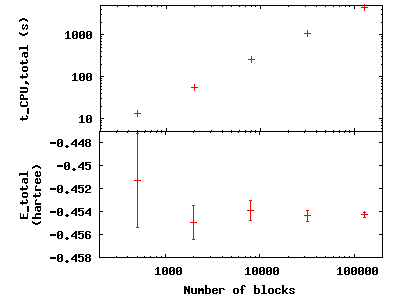
\includegraphics[trim = 0mm 0mm 0mm 0mm, clip,width=0.75\columnwidth]{./figures/lab_qmc_statistics_blocks.png}
\end{center}
\end{figure}
\FloatBarrier

%\includegraphics[scale=1.0]{nblock_vs_tcpu_energy_H_STO-2G.png}

Press \textbf{q [Enter]} to quit gnuplot.

\subsection{Improving the basis set}

In all of the above examples, we are using the sum of two gaussian functions
(STO-2G) to approximate what should be a simple decaying exponential (STO =
Slater-type orbital) for the wave function of the ground state of the hydrogen
atom.  The sum of multiple copies of a function varying each copy's width and
amplitude with coefficients is called a \textit{basis set}. As we add gaussians
to the basis set, the approximation improves, the variance goes toward zero and
the energy goes to -0.5 hartrees.  In nearly every other case, the exact
function is unknown, and we add basis functions until the total energy does not
change within some threshold.

Change to the directory \ishell{basis} and look at the total energy and
variance as we change the wave function by typing \textbf{qmca -q ev H\_*}:

\begin{shade}
                            LocalEnergy               Variance        ratio 
H_STO-2G  series 0  -0.454460 +/- 0.000568   0.529496 +/- 0.018445   1.1651 
H_STO-3G  series 0  -0.465386 +/- 0.000502   0.410491 +/- 0.010051   0.8820 
H_STO-6G  series 0  -0.471332 +/- 0.000491   0.213919 +/- 0.012954   0.4539 
H__exact  series 0  -0.500000 +/- 0.000000   0.000000 +/- 0.000000   -0.0000 
\end{shade}

qmca also puts out the ratio of the variance to the local energy in a column to
the right of the variance error bar.  A typical high quality value for this
ratio is lower than 0.1 or so--none of these few-gaussian wave functions
satisfy that rule of thumb.

Use qmca to plot the trace of the local energy, kinetic energy, and potential
energy of H\_\_exact--the total energy is constantly -0.5 hartree even though
the kinetic and potential energies fluctuate from configuration to
configuration.

\subsection{Adding a Jastrow factor}

Another route to reducing the variance is the introduction of a Jastrow factor to 
account for electron-electron correlation (not the statistical autocorrelation
of Monte Carlo steps but the physical avoidance that electrons have of one another).
To do this, we will switch to the hydrogen dimer with the exact ground state
wave function of the atom (STO basis)--this will not be exact for the dimer.
The ground state energy of the hydrogen dimer is -1.174 hartrees.

Change directories to \ishell{dimer} and put in \textbf{qmca -q ev *scalar.dat}
to see the result of adding a simple, one-parameter Jastrow to the STO basis
for the hydrogen dimer at experimental bond length:

\begin{shade}
                               LocalEnergy               Variance           
H2_STO___no_jastrow  series 0  -0.876548 +/- 0.005313   0.473526 +/- 0.014910
H2_STO_with_jastrow  series 0  -0.912763 +/- 0.004470   0.279651 +/- 0.016405
\end{shade}

The energy reduces by 0.044 +/- 0.006 hartrees and the variance by 0.19 +/- 0.02.
This is still 20\% above the ground state energy, and subsequent labs will cover how
to improve on this with improved forms of the wave function that capture more
of the physics.

\section{Scaling to larger numbers of electrons}

\subsection{Calculating the efficiency}

The inverse of the product of CPU time and the variance measures the
\textit{efficiency} of an MC calculation.  Use qmca to calculate efficiency by
typing \textbf{qmca -q eff *scalar.dat} to see the efficiency of these two
H$_2$ calculations:

\begin{shade}
H2_STO___no_jastrow  series 0  Efficiency = 16698.725453 +/- 0.000000 
H2_STO_with_jastrow  series 0  Efficiency = 52912.365609 +/- 0.000000 
\end{shade}

The Jastrow factor increased the efficiency in these calculations by a factor
of three, largely through the reduction in variance (check the average block
CPU time to verify this claim).

\subsection{Scaling up}

To see how MC scales with increasing particle number, change directories to
\ishell{size}.  Here are the data from runs of increasing number of electrons
for H, H$_2$, C, CH$_4$, C$_2$, C$_2$H$_4$, (CH$_4$)$_2$, and (C$_2$H$_4$)$_2$
using the STO-6G basis set for the orbitals of the Slater determinant.  The file names begin with the number of electrons simulated for those data.

Use \textbf{qmca -q bc *scalar.dat} to see that the CPU time per block
increases with number of electrons in the simulation, then plot the total CPU
time of the simulation by \textbf{gnuplot Nelectron\_tCPU.plt}:

\FloatBarrier
\begin{figure}[ht!]
\begin{center}
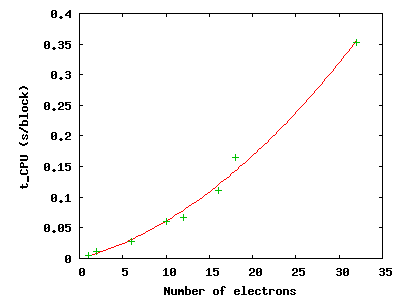
\includegraphics[trim = 0mm 0mm 0mm 0mm, clip,width=0.75\columnwidth]{./figures/lab_qmc_statistics_scaling.png}
\end{center}
\end{figure}
\FloatBarrier

%\includegraphics[scale=1.0]{nelectron_vs_tcpu_H_C_CH_STO-6G.png}

The green pluses represent the CPU time per block at each electron number.
The red line is a quadratic fit to those data.  For a fixed basis set size, we expect the time to scale quadratically up to 1000s of electrons, at which point a cubic scaling term may become dominant.  Knowing the scaling allows you to roughly project the calculation time for a larger number of electrons.

Press \textbf{q [Enter]} to quit gnuplot.

This isn't the whole story, however.  The variance of the energy also increases
with a fixed basis set as the number of particles increases at a faster rate
than the energy decreases.  To see this, type \textbf{qmca -q ev *scalar.dat}:

\begin{shade}
                            LocalEnergy               Variance           
01________H  series 0  -0.471352 +/- 0.000493      0.213020 +/- 0.012950 
02_______H2  series 0  -0.898875 +/- 0.000998      0.545717 +/- 0.009980 
06________C  series 0  -37.608586 +/- 0.020453   184.322000 +/- 45.481193
10______CH4  series 0  -38.821513 +/- 0.022740   169.797871 +/- 24.765674
12_______C2  series 0  -72.302390 +/- 0.037691   491.416711 +/- 106.090103
16_____C2H4  series 0  -75.488701 +/- 0.042919   404.218115 +/- 60.196642
18___CH4CH4  series 0  -58.459857 +/- 0.039309   498.579645 +/- 92.480126
32_C2H4C2H4  series 0  -91.567283 +/- 0.048392   632.114026 +/- 69.637760
\end{shade}

The increase in variance is not uniform, but the general trend is upward with a
fixed wave function form and basis set.  Subsequent labs will address how to
improve the wave function in order to keep the variance manageable.

\chapter{Lab 2: QMC Basics}
\label{chap:lab_qmc_basics}



\section{Topics covered in this Lab}
This lab focuses on the basics of performing quality QMC calculations.  As an example participants test an oxygen pseudopotential within DMC by calculating atomic and dimer properties, a common step prior to production runs.  Topics covered include:
\begin{itemize}
  \item{converting pseudopotentials into QMCPACK's FSATOM format}
  \item{generating orbitals with Quantum ESPRESSO}
  \item{converting orbitals into QMCPACK's ESHDF format with pw2qmcpack}
  \item{optimizing Jastrow factors with QMCPACK}
  \item{removing DMC timestep error via extrapolation}
  \item{automating QMC workflows with Nexus}
  \item{testing pseudopotentials for accuracy}
  \hide{
  \item{(optional) running QMCPACK for a general system of interest}
  }
\end{itemize}

\section{Lab outline}
\begin{enumerate}
  \item{download and conversion of oxygen atom pseudopotential}
  \item{DMC timestep study of the neutral oxygen atom}
  \begin{enumerate}
    \item{DFT orbital generation with Quantum ESPRESSO}
    \item{orbital conversion with \ishell{pw2qmcpack.x}}
    \item{optimization of Jastrow correlation factor with QMCPACK}
    \item{DMC run with multiple timesteps}
  \end{enumerate}
  \item{DMC timestep study of the first ionization potential of oxygen}
  \begin{enumerate}
    \item{repetition of a-d above for ionized oxygen atom}
  \end{enumerate}
  \item{automated DMC calculations of the oxygen dimer binding curve}
\end{enumerate}


\section{Lab directories and files}
\footnotesize
\begin{verbatim}%
labs/lab2_qmc_basics/
│
├── oxygen_atom           - oxygen atom calculations 
│   ├── O.q0.dft.in          - Quantum ESPRESSO input for DFT run
│   ├── O.q0.p2q.in          - pw2qmcpack.x input for orbital conversion run
│   ├── O.q0.opt.in.xml      - QMCPACK input for Jastrow optimization run
│   ├── O.q0.dmc.in.xml      - QMCPACK input file for neutral O DMC
│   ├── ip_conv.py           - tool to fit oxygen IP vs timestep
│   └── reference            - directory w/ completed runs
│
├── oxygen_dimer          - oxygen dimer calculations
│   ├── dimer_fit.py         - tool to fit dimer binding curve
│   ├── O_dimer.py           - automation script for dimer calculations
│   ├── pseudopotentials     - directory for pseudopotentials
│   └── reference            - directory w/ completed runs
│
└── your_system           - performing calculations for an arbitrary system (yours)
    ├── example.py           - example nexus file for periodic diamond
    ├── pseudopotentials     - directory containing C pseudopotentials
    └── reference            - directory w/ completed runs
\end{verbatim}
\normalsize

\section{Obtaining and converting a pseudopotential for oxygen}
\label{sec:lqb_pseudo}
First enter the \ishell{oxygen\_atom} directory:
\begin{shade}
cd labs/lab2_qmc_basics/oxygen_atom/
\end{shade}
\noindent
Throughout the rest of the lab, locations will be specified with respect to \ishell{labs/lab2\_qmc\_basics} (e.g. \ishell{oxygen\_atom}).

We will use a potential from the Burkatzki-Filippi-Dolg pseudopotential database.  
Although the full database is available in QMCPACK distribution (\ishell{trunk/pseudopotentials/BFD/}), 
we use a BFD pseudopotential to illustrate the process of converting and testing an 
external potential for use with QMCPACK.   To obtain the pseudopotential, go to 
\href{http://www.burkatzki.com/pseudos/index.2.html}{http://www.burkatzki.com/pseudos/index.2.html}
and click on the ``Select Pseudopotential'' button.  Next click on oxygen in the 
periodic table.  Click on the empty circle next to ``V5Z'' (a large gaussian 
basis set) and click on ``Next''.  Select the Gamess format and click on 
``Retrive Potential''.  Helpful information about the pseudopotential will be 
displayed.  The desired portion is at the bottom (the last 7 lines).  Copy 
this text into the editor of your choice (e.g. \ishell{emacs} or \ishell{vi}) 
and save it as \ishell{O.BFD.gamess} 
(be sure to include a newline at the end of the file).  To transform the 
pseudopotential into the FSATOM XML format used by QMCPACK, use the \ishell{ppconvert} 
tool:

\noindent
\ifws
\begin{shade}
ppconvert --gamess_pot O.BFD.gamess --s_ref "1s(2)2p(4)" \
 --p_ref "1s(2)2p(4)" --d_ref "1s(2)2p(4)" --xml O.BFD.xml
\end{shade}
\else
\begin{shade}
jobrun_vesta ppconvert --gamess_pot O.BFD.gamess --s_ref "1s(2)2p(4)" \
 --p_ref "1s(2)2p(4)" --d_ref "1s(2)2p(4)" --xml O.BFD.xml
\end{shade}
\fi

\noindent
Observe the notation used to describe the reference valence configuration for this helium-core PP: \ishell{1s(2)2p(4)}.  The \ishell{ppconvert} tool uses the following convention for the valence states: the first $s$ state is labeled \ishell{1s} (\ishell{1s}, \ishell{2s}, \ishell{3s}, \ldots), the first $p$ state is labeled \ishell{2p} (\ishell{2p}, \ishell{3p}, \ldots), the first $d$ state is labeled \ishell{3d} (\ishell{3d}, \ishell{4d}, \ldots). Copy the resulting xml file into the \ishell{oxygen\_atom} directory.

Note: the command to convert the PP into QM Espresso's UPF format is similar (both formats are required):

\noindent
\ifws
\begin{shade}
ppconvert --gamess_pot O.BFD.gamess --s_ref "1s(2)2p(4)" \
 --p_ref "1s(2)2p(4)" --d_ref "1s(2)2p(4)" --log_grid --upf O.BFD.upf
\end{shade}
\else
\begin{shade}
jobrun_vesta ppconvert --gamess_pot O.BFD.gamess --s_ref "1s(2)2p(4)" \
 --p_ref "1s(2)2p(4)" --d_ref "1s(2)2p(4)" --log_grid --upf O.BFD.upf
\end{shade}
\noindent
\fi

For reference, the text of \ishell{O.BFD.gamess} should be:
\begin{lstlisting}
O-QMC GEN 2 1
3
6.00000000 1 9.29793903
55.78763416 3 8.86492204
-38.81978498 2 8.62925665
1
38.41914135 2 8.71924452

\end{lstlisting}
\noindent
The full QMCPACK pseudopotential is also included in \ishell{oxygen\_atom/reference/O.BFD.*}.


\section{DFT with Quantum ESPRESSO to obtain the orbital part of the wavefunction}
\label{sec:lqb_dft}
With the pseudopotential in hand, the next step toward a QMC calculation is to obtain the Fermionic part of the wavefunction, in this case a single Slater determinant constructed from DFT-LDA orbitals for a neutral oxygen atom.  If you had trouble with the pseudopotential conversion step, pre-converted pseudopotential files are located in the \ishell{oxygen\_atom/reference} directory.  

Quantum ESPRESSO input for the DFT-LDA ground state of the neutral oxygen atom can be found in \ishell{O.q0.dft.in} and also listing \ref{lst:O_q0_dft} below.  Setting \ishell{wf\_collect=.true.} instructs Quantum Espresso to write the orbitals to disk at the end of the run. Option \ishell{wf\_collect=.true.} may be a potential problem in large simulations, it is recommended to avoid it and use the converter pw2qmcpack in parallel, see details in Sec.~\ref{sec:pw2qmcpack}. Note that the plane-wave energy cutoff has been set to a reasonable value of 300 Ry here (\ishell{ecutwfc=300}).  This value depends on the pseudopotentials used, and in general should be selected by running DFT$\rightarrow$(orbital conversion)$\rightarrow$VMC with increasing energy cutoffs until the lowest VMC total energy and variance is reached.

\begin{lstlisting}[style=ESPRESSO, language=espresso, caption={Quantum ESPRESSO input file for the neutral oxygen atom (\ishell{O.q0.dft.in})\label{lst:O_q0_dft}}]
&CONTROL
   calculation       = 'scf'
   restart_mode      = 'from_scratch'
   prefix            = 'O.q0'
   outdir            = './'
   pseudo_dir        = './'
   disk_io           = 'low'
   wf_collect        = .true.
/

&SYSTEM
   celldm(1)         = 1.0
   ibrav             = 0
   nat               = 1
   ntyp              = 1
   nspin             = 2
   tot_charge        = 0
   tot_magnetization = 2
   input_dft         = 'lda'
   ecutwfc           = 300
   ecutrho           = 1200
   nosym             = .true.
   occupations       = 'smearing'
   smearing          = 'fermi-dirac'
   degauss           = 0.0001
/

&ELECTRONS
   diagonalization   = 'david'
   mixing_mode       = 'plain'
   mixing_beta       = 0.7
   conv_thr          = 1e-08
   electron_maxstep  = 1000
/


ATOMIC_SPECIES 
   O  15.999 O.BFD.upf

ATOMIC_POSITIONS alat
   O     9.44863067       9.44863161       9.44863255

K_POINTS automatic
   1 1 1  0 0 0 

CELL_PARAMETERS cubic
        18.89726133       0.00000000       0.00000000 
         0.00000000      18.89726133       0.00000000 
         0.00000000       0.00000000      18.89726133
\end{lstlisting}

Run Quantum ESPRESSO by typing 
\ifws
\begin{shade}
mpirun -np 4 pw.x -input O.q0.dft.in >&O.q0.dft.out&
\end{shade}
\else
\begin{shade}
jobrun_vesta pw.x O.q0.dft.in
\end{shade}
\fi

The DFT run should take a few minutes to complete.  If desired, you can track the progress of the DFT run by typing ``\ifws\ishell{tail -f O.q0.dft.out}
\else\ishell{tail -f O.q0.dft.output}\fi''. Once finished, you should check the LDA total energy in \ifws\ishell{O.q0.dft.out}\else\ishell{O.q0.dft.output}\fi by typing ``\ifws\ishell{grep '!  ' O.q0.dft.out}\else\ishell{grep '!  ' O.q0.dft.output}\fi''.  The result should be close to
\begin{shade}
!    total energy              =     -31.57553905 Ry
\end{shade} 
% both of the numbers below are for 200 Ry (too small as it turns out)
% 10 Angstrom cell
%!    total energy              =     -31.56729415 Ry
% 15 Angstrom cell
%!    total energy              =     -31.56730213 Ry



The orbitals have been written in a format native to Quantum ESPRESSO in the \ishell{O.q0.save} directory.  We will convert them into the ESHDF format expected by QMCPACK by using the \ishell{pw2qmcpack.x} tool.  The input for \ishell{pw2qmcpack.x} can be found in the file \ishell{O.q0.p2q.in} and also in listing \ref{lst:O_q0_p2q} below. 

\begin{lstlisting}[caption={\ishell{pw2qmcpack.x} input file for orbital conversion (\ishell{O.q0.p2q.in})\label{lst:O_q0_p2q}}]
&inputpp
  prefix     = 'O.q0'
  outdir     = './'
  write_psir = .false.
/
\end{lstlisting}

Perform the orbital conversion now by typing the following:
\ifws
\begin{shade}
mpirun -np 1 pw2qmcpack.x<O.q0.p2q.in>&O.q0.p2q.out&
\end{shade}
\else
\begin{shade}
jobrun_vesta pw2qmcpack.x O.q0.p2q.in
\end{shade}
\fi
\noindent
Upon completion of the run, a new file should be present containing the orbitals for QMCPACK: \ishell{O.q0.pwscf.h5}.  Template XML files for particle (\ishell{O.q0.ptcl.xml}) and wavefunction (\ishell{O.q0.wfs.xml}) inputs to QMCPACK should also be present.  


\section{Optimization with QMCPACK to obtain the correlated part of the wavefunction}\label{sec:optimization_walkthrough}
The wavefunction we have obtained to this point corresponds to a non-interacting Hamiltonian.  Once the Coulomb pair potential is switched on between particles, it is known analytically that the exact wavefunction has cusps whenever two particles meet spatially and in general the electrons become correlated.  This is represented in the wavefunction by introducing a Jastrow factor containing at least pair correlations
\begin{align}
  &\Psi_{Slater-Jastrow}=e^{-J}\Psi_{Slater} \\
  &J = \sum_{\sigma\sigma'}\sum_{i<j}u^{\sigma\sigma'}_2(|r_i-r_j|) + \sum_\sigma\sum_{iI}u^{\sigma I}_1(|r_i-r_I|)
\end{align}
Here $\sigma$ is a spin variable while $r_i$ and $r_I$ represent electron and ion coordinates, respectively.  The introduction of $J$ into the wavefunction is similar to F12 methods in quantum chemistry, though it has been present in essentially all QMC studies since the first applications the method (circa 1965).

How are the functions $u_2^{\sigma\sigma'}$ and $u_1^{\sigma}$ obtained?  Generally, they are approximated by analytical functions with several unknown parameters that are determined by minimizing the energy or variance directly within VMC.  This is effective because the energy and variance reach a global minimum only for the true ground state wavefunction ($\textrm{Energy}=E\equiv\expval{\Psi}{\hat{H}}{\Psi}$, $\textrm{Variance}=V\equiv\expval{\Psi}{(\hat{H}-E)^2}{\Psi}$).  For this exercise, we will focus on minimizing the variance.

% background on the wavefunction should be covered elsewhere in the manual
%   perhaps replace this with just the figure and a couple of brief comments 
\hide{
\subsubsection{Background on trial wavefunction and optimization}\label{sec:opt_background}
The trial wavefunction used to describe the neutral oxygen atom is of the 
standard Slater-Jastrow form:
\begin{align}  
  \Psi_T = e^{-(J_1+J_2)}D^\uparrow(\{\phi_u^\uparrow\}_{u=1}^{N^\uparrow})D^\downarrow(\{\phi_d^\downarrow\}_{d=1}^{N^\uparrow})
\end{align}
The orbitals forming the spin-restricted Slater determinants 
($D^\uparrow/D^\downarrow$) are obtained from DFT or Hartree-Fock (\emph{e.g.} via Quantum ESPRESSO) 
and are fixed.  The ground state of the (pseudo) oxygen atom is spin polarized 
with $N^{\uparrow}=4$ and $N^{\downarrow}=2$.  

The part of the wavefunction we will be optimizing is the Jastrow factor 
($e^{-(J_1+J_2)}$), which in this case includes one- (electron-ion) and two- 
(electron-electron) body correlation functions.  The Jastrow factor is symmetric 
under same-spin electron exchange and does not affect the DMC fixed node 
approximation.  Optimization of the Jastrow factor does, however, improve the 
efficiency of the DMC calculation and reduces additional approximations due to 
non-local pseudopotentials (locality approximation, T-moves).  Note that a three-body 
term ($J_3$) is also available and is often necessary when using pseudopotentials 
for transition metal species or when high accuracy is desired for molecules.  


\begin{figure}
\begin{center}
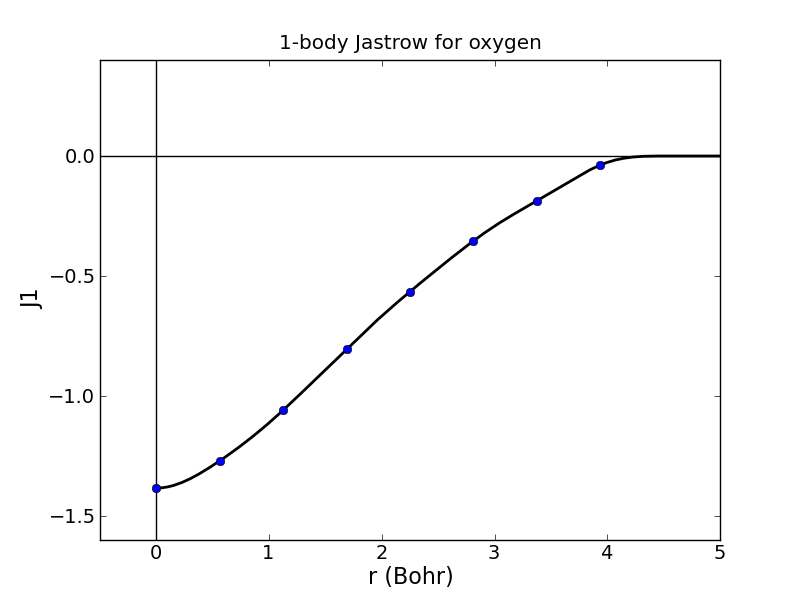
\includegraphics[trim = 0mm 0mm 0mm 0mm, clip,width=0.75\columnwidth]{./figures/lab_qmc_basics_J1.png}
\end{center}
\caption{Optimized $U_1$ function for 1-body Jastrow factor of an oxygen atom.
\label{fig:u1_spline}
}
\end{figure}

The explicit form of the one-body Jastrow factor we will be using is
\begin{align}\label{eq:J1}
  J_1 = \sum_{e=1}^{N^\uparrow+N^\downarrow}U_1^{\uparrow/\downarrow}(|r_e-r_O|)
\end{align}
where $r_e$ refers to the electron positions and $r_O$ is 
the position of the oxygen ion.  The $U_1^{\uparrow/\downarrow}$ term is a 
one-dimensional radial function represented with piecewise continuous cubic 
polynomials (B-splines).  The adjustable parameters to be optimized are the 
``knots'' of the B-splines which are simply the values of the $U_1$ function at 
uniformly spaced grid points (See fig. \ref{fig:u1_spline} for an example of a $U_1$ 
spline function with 8 knots).  

The two-body Jastrow factor is spin resolved ($r^\uparrow/r^\downarrow$ are up/down electron positions):
\begin{align}\label{eq:J2}
  J_2 = \sum_{u<u'}U_2^{\uparrow\uparrow/\downarrow\downarrow}(|r_u^\uparrow-r_{u'}^\uparrow|) + \sum_{d<d'}U_2^{\uparrow\uparrow/\downarrow\downarrow}(|r_d^\downarrow-r_{d'}^\downarrow|) + \sum_{u,d} U_2^{\uparrow\downarrow}(|r_u^\uparrow-r_d^\downarrow|)
\end{align}
For an atom, Pad\'{e} functions are appropriate for $U_2^{\uparrow\uparrow/\downarrow\downarrow}$ and $U_2^{\uparrow\downarrow}$:
\begin{align}
  U_2(r) = \frac{Ar}{1+Br}
\end{align}
Only $B^{\uparrow\uparrow/\downarrow\downarrow}$ and $B^{\uparrow\downarrow}$ are adjustable since the $A$ parameters are fixed by the electron-electron cusp conditions.

Wavefunction optimization essentially relies on two inequalities regarding energy and variance:
\begin{align}
  E_T(P) &= \frac{\expvalh{\Psi_T(P)}{H}{\Psi_T(P)}}{\overlap{\Psi_T(P)}{\Psi_T(P)}} \ge E_0 \\
  V_T(P) &= \frac{\expval{\Psi_T(P)}{\hat{H}^2}{\Psi_T(P)}}{\overlap{\Psi_T(P)}{\Psi_T(P)}} - \left(\frac{\expval{\Psi_T(P)}{H}{\Psi_T(P)}}{\overlap{\Psi_T(P)}{\Psi_T(P)}}\right)^2 \ge 0   
\end{align}
Here $E_0$ is the ground state energy, $E_T(P)$ is the trial energy, $V_T(P)$ is the trial variance, and $P$ denotes the set of adjustable parameters in the trial wavefunction.  Equality is reached only for the true ground state wavefunction and so the trial wavefunction can be improved by attempting to minimize a chosen cost function: 
\begin{align}
  C(P) = \alpha E_T(P) + (1-\alpha) V_T(P).
\end{align}  
Iterative varational Monte Carlo methods have been developed to handle the non-linear optimization problem $\min\limits_P C(P)$.  We will be using the linearized optimization method of Umrigar, \emph{et al.} (PRL \textbf{98} 110201 (2007)).  Let us try this now with QMCPACK.
}

First, we need to update the template particle and wavefunction information in \ishell{O.q0.ptcl.xml} and \ishell{O.q0.wfs.xml}.  We want to simulate the O atom in open boundary conditions (the default is periodic).  To do this open \ishell{O.q0.ptcl.xml} with your favorite text editor (e.g. \ishell{emacs} or \ishell{vi}) and replace
\begin{lstlisting}[style=QMCPXML]
<parameter name="bconds">
   p p p
</parameter>
<parameter name="LR_dim_cutoff">
   15
</parameter>
\end{lstlisting}
with
\begin{lstlisting}[style=QMCPXML]
<parameter name="bconds">
   n n n 
</parameter>
\end{lstlisting}

Next we will select Jastrow factors appropriate for an atom.  In open boundary conditions, the B-spline Jastrow correlation functions should cut off to zero at some distance away from the atom.  Open \ishell{O.q0.wfs.xml} and add the following cutoffs (\ishell{rcut} in Bohr radii) to the correlation factors:
\begin{lstlisting}[style=QMCPXML]
...
<correlation speciesA="u" speciesB="u" size="8" rcut="10.0">
...
<correlation speciesA="u" speciesB="d" size="8" rcut="10.0">
...
<correlation elementType="O" size="8" rcut="5.0">
...
\end{lstlisting}
\noindent
These terms correspond to $u_2^{\uparrow\uparrow}/u_2^{\downarrow\downarrow}$, $u_2^{\uparrow\downarrow}$, and $u_1^{\uparrow O}/u_1^{\downarrow O}$, respectively.  In each case, the correlation function ($u_*$) is represented by piecewise continuous cubic B-splines.  Each correlation function has eight parameters which are just the values of $u$ on a uniformly spaced grid up to \ishell{rcut}.  Initially the parameters (\ishell{coefficients}) are set to zero:
\begin{lstlisting}[style=QMCPXML]
<correlation speciesA="u" speciesB="u" size="8" rcut="10.0">
  <coefficients id="uu" type="Array">
     0.0 0.0 0.0 0.0 0.0 0.0 0.0 0.0
  </coefficients>
</correlation>
\end{lstlisting}

Finally, we need to assemble particle, wavefunction, and pseudopotential information into the main QMCPACK input file (\ishell{O.q0.opt.in.xml}) and specify inputs for the Jastrow optimization process.  Open \ishell{O.q0.opt.in.xml} and write in the location of the particle, wavefunction, and pseudopotential files (``\ishell{<!-- ... -->}'' are comments):
\begin{lstlisting}[style=QMCPXML]
...
<!-- include simulationcell and particle information from pw2qmcpqack -->
<include href="O.q0.ptcl.xml"/>
...
<!-- include wavefunction information from pw2qmcpqack -->
<include href="O.q0.wfs.xml"/>
...
<!-- O pseudopotential read from "O.BFD.xml" -->
<pseudo elementType="O" href="O.BFD.xml"/>
...
\end{lstlisting}
\noindent
The relevant portion of the input describing the linear optimization process is
\begin{lstlisting}[style=QMCPXML]
<loop max="MAX">  
  <qmc method="linear" move="pbyp" checkpoint="-1">
    <cost name="energy"              >  ECOST    </cost>
    <cost name="unreweightedvariance">  UVCOST   </cost>
    <cost name="reweightedvariance"  >  RVCOST   </cost>
    <parameter name="timestep"       >  TS       </parameter>
    <parameter name="samples"        >  SAMPLES  </parameter>
    <parameter name="warmupSteps"    >  50       </parameter>
    <parameter name="blocks"         >  200      </parameter>
    <parameter name="subSteps"       >  1        </parameter>
    <parameter name="nonlocalpp"     >  yes      </parameter>
    <parameter name="useBuffer"      >  yes      </parameter>
    ...
  </qmc>
</loop>
\end{lstlisting}
\noindent
An explanation of each input variable can be found below.  The remaining variables control specialized internal details of the linear optimization algorithm.  The meaning of these inputs is beyond the scope of this lab and reasonable results are often obtained keeping these values fixed. 
\begin{description}
  \item[energy] Fraction of trial energy in the cost function.
  \item[unreweightedvariance] Fraction of unreweighted trial variance in the cost function.  Neglecting the weights can be more robust.
  \item[reweightedvariance] Fraction of trial variance (including the full weights) in the cost function.  
  \item[timestep] Timestep of the VMC random walk, determines spatial distance moved by each electron during MC steps.  Should be chosen such that the acceptance ratio of MC moves is around 50\% (30-70\% is often acceptable).  Reasonable values are often between 0.2 and 0.6 $\textrm{Ha}^{-1}$.
  \item[samples] Total number of MC samples collected for optimization, determines statistical error bar of cost function.  Often efficient to start with a modest number of samples (50k) and then increase as needed.  More samples may be required if the wavefunction contains a large number of variational parameters.  MUST be be a multiple of the number of threads/cores \labsw{}{(use multiples of 512 on Vesta)}.
  \item[warmupSteps]  Number of MC steps discarded as a warmup or equilibration period of the random walk.  If this is too small, it will bias the optimization procedure.
  \item[blocks]  Number of average energy values written to output files.  Should be greater than 200 for meaningful statistical analysis of output data (\emph{e.g.} via \ishell{qmca}).
  \item[subSteps] Number of MC steps in between energy evaluations.  Each energy evaluation is expensive so taking a few steps to decorrelate between measurements can be more efficient.  Will be less efficient with many substeps.
  \item[nonlocalpp,useBuffer] If \ishell{nonlocalpp="no"}, then nonlocal part of the pseudopotential is not included when computing the cost function.  If \ishell{useBuffer="yes"}, then temporary data is stored to speed up nonlocal pseudopotential evaluation at the expense of memory consumption.  
  \item[loop max] Number of times to repeat the optimization.  Using the resulting wavefunction from the previous optimization in the next one improves the results.  Typical choices range between 8 and 16.   
\end{description}
The cost function defines the quantity to be minimized during optimization. The three components of the cost function, energy, unreweighted variance, and reweighted variance should sum to one.  Dedicating 100\% of the cost function to unreweighted variance is often a good choice.  Another common choice is to try 90/10 or 80/20 mixtures of reweighted variance and energy.  Using 100\% energy minimization is desirable for reducing DMC pseudopotential localization errors, but the optimization process is less stable and should only be attempted after performing several cycles of e.g. variance minimization first (the entire \ishell{loop} section can be duplicated with a different cost function each time).

Replace \ishell{MAX}, \ishell{EVCOST}, \ishell{UVCOST}, \ishell{RVCOST}, \ishell{TS}, and \ishell{SAMPLES} in the \ishell{loop} with appropriate starting values in the \ishell{O.q0.opt.in.xml} input file.  Perform the optimization run by typing
\ifws
\begin{shade}
mpirun -np 4 qmcpack O.q0.opt.in.xml >&O.q0.opt.out&
\end{shade}
\else
\begin{shade}
jobrun_vesta qmcpack O.q0.opt.in.xml
\end{shade}
\fi
\noindent
The run should only take a few minutes for reasonable values of loop \ishell{max} and \ishell{samples}.  

Log file output will appear in \labsw{\ishell{O.q0.opt.out}}{\ishell{O.q0.opt.output}}.  The beginning of each linear optimization will be marked with text similar to
\begin{shade}
=========================================================
  Start QMCFixedSampleLinearOptimize
  File Root O.q0.opt.s011 append = no 
=========================================================
\end{shade}
\noindent
At the end of each optimization section the change in cost function, new values for the Jastrow parameters, and elapsed wallclock time are reported:
\begin{shade}
 OldCost: 7.0598901869e-01 NewCost: 7.0592576381e-01 Delta Cost:-6.3254886314e-05
...
  <optVariables href="O.q0.opt.s011.opt.xml">
uu_0 6.9392504232e-01 1 1  ON 0
uu_1 4.9690781460e-01 1 1  ON 1
uu_2 4.0934542375e-01 1 1  ON 2
uu_3 3.7875640157e-01 1 1  ON 3
uu_4 3.7308380014e-01 1 1  ON 4
uu_5 3.5419786809e-01 1 1  ON 5
uu_6 4.3139019377e-01 1 1  ON 6
uu_7 1.9344371667e-01 1 1  ON 7
ud_0 3.9219009713e-01 1 1  ON 8
ud_1 1.2352664647e-01 1 1  ON 9
ud_2 4.4048945133e-02 1 1  ON 10
ud_3 2.1415676741e-02 1 1  ON 11
ud_4 1.5201803731e-02 1 1  ON 12
ud_5 2.3708169445e-02 1 1  ON 13
ud_6 3.4279064930e-02 1 1  ON 14
ud_7 4.3334583596e-02 1 1  ON 15
eO_0 -7.8490123937e-01 1 1  ON 16
eO_1 -6.6726618338e-01 1 1  ON 17
eO_2 -4.8753453838e-01 1 1  ON 18
eO_3 -3.0913993774e-01 1 1  ON 19
eO_4 -1.7901872177e-01 1 1  ON 20
eO_5 -8.6199000697e-02 1 1  ON 21
eO_6 -4.0601160841e-02 1 1  ON 22
eO_7 -4.1358075061e-03 1 1  ON 23
  </optVariables>
...
  QMC Execution time = 2.8218972974e+01 secs
\end{shade}
\noindent
The cost function should decrease during each linear optimization (\ishell{Delta cost < 0}).  Try ``\labsw{\ishell{grep OldCost *opt.out}}{\ishell{grep OldCost *opt.output}}''.  You should see something like this:
\begin{shade}
 OldCost: 1.2655186572e+00 NewCost: 7.2443875597e-01 Delta Cost:-5.4107990118e-01
 OldCost: 7.2229830632e-01 NewCost: 6.9833678217e-01 Delta Cost:-2.3961524143e-02
 OldCost: 8.0649629434e-01 NewCost: 8.0551871147e-01 Delta Cost:-9.7758287036e-04
 OldCost: 6.6821241388e-01 NewCost: 6.6797703487e-01 Delta Cost:-2.3537901148e-04
 OldCost: 7.0106275099e-01 NewCost: 7.0078055426e-01 Delta Cost:-2.8219672877e-04
 OldCost: 6.9538522411e-01 NewCost: 6.9419186712e-01 Delta Cost:-1.1933569922e-03
 OldCost: 6.7709626744e-01 NewCost: 6.7501251165e-01 Delta Cost:-2.0837557922e-03
 OldCost: 6.6659923822e-01 NewCost: 6.6651737755e-01 Delta Cost:-8.1860671682e-05
 OldCost: 7.7828995609e-01 NewCost: 7.7735482525e-01 Delta Cost:-9.3513083900e-04
 OldCost: 7.2717974404e-01 NewCost: 7.2715201115e-01 Delta Cost:-2.7732880747e-05
 OldCost: 6.9400639873e-01 NewCost: 6.9257183689e-01 Delta Cost:-1.4345618444e-03
 OldCost: 7.0598901869e-01 NewCost: 7.0592576381e-01 Delta Cost:-6.3254886314e-05
\end{shade}

Blocked averages of energy data, including the kinetic energy and components of the potential energy, are written to \ishell{scalar.dat} files.  The first is named ``\ishell{O.q0.opt.s000.scalar.dat}'', with a series number of zero (\ishell{s000}).  In the end there will be \ishell{MAX} of them, one for each series. 

When the job has finished, use the \ishell{qmca} tool to assess the effectiveness of the optimization process.  To look at just the total energy and the variance, type ``\ishell{qmca -q ev O.q0.opt*scalar*}''.  This will print the energy, variance, and the variance/energy ratio in Hartree units:
\begin{shade}
                            LocalEnergy               Variance           ratio
O.q0.opt  series 0  -15.739585 +/- 0.007656   0.887412 +/- 0.010728   0.0564
O.q0.opt  series 1  -15.848347 +/- 0.004089   0.318490 +/- 0.006404   0.0201
O.q0.opt  series 2  -15.867494 +/- 0.004831   0.292309 +/- 0.007786   0.0184
O.q0.opt  series 3  -15.871508 +/- 0.003025   0.275364 +/- 0.006045   0.0173
O.q0.opt  series 4  -15.865512 +/- 0.002997   0.278056 +/- 0.006523   0.0175
O.q0.opt  series 5  -15.864967 +/- 0.002733   0.278065 +/- 0.004413   0.0175
O.q0.opt  series 6  -15.869644 +/- 0.002949   0.273497 +/- 0.006141   0.0172
O.q0.opt  series 7  -15.868397 +/- 0.003838   0.285451 +/- 0.007570   0.0180
...
\end{shade}
\noindent
Plots of the data can also be obtained with the ``\ishell{-p}'' option (``\ishell{qmca -p -q ev O.q0.opt*scalar*}'').

Identify which optimization series is the ``best'' according to your cost function.  It is likely that multiple series are similar in quality.  Note the \ishell{opt.xml} file corresponding to this series.  This file contains the final value of the optimized Jastrow parameters to be used in the DMC calculations of the next section of the lab.  

\vspace{1cm}
\begin{flushleft}
\textbf{\underline{Questions and Exercises}}
\end{flushleft}
\begin{enumerate}
  \item{What is the acceptance ratio of your optimization runs? (use ``\ishell{qmca -q ar O.q0.opt*scalar*}'')  Do you expect the Monte Carlo sampling to be efficient?}
  \item{How do you know when the optimization process has converged?}
%  \item{Why is the mean and the error of the variance sometimes large?  Consider using \newline``\ishell{qmca -t -q ev O.q0.opt*scalar*}'' to investigate.}
  \item{(optional) Optimization is sometimes sensitive to initial guesses of the parameters.  If you have time, try varying the initial parameters, including the cutoff radius (\ishell{rcut}) of the Jastrow factors (remember to change \ishell{id} in the \ishell{<project/>} element).  Do you arrive at a similar set of final Jastrow parameters?  What is the lowest variance you are able to achieve?}
\end{enumerate}



\section{DMC timestep extrapolation I: neutral O atom}
The diffusion Monte Carlo (DMC) algorithm contains two biases in addition to the fixed node and pseudopotential approximations that are important to control: timestep and population control bias.  In this section we will focus on estimating and removing timestep bias from DMC calculations.  The essential fact to remember is that the bias vanishes as the timestep goes to zero while the needed computer time increases inversely with the timestep.   


% background on timestep error should be covered elsewhere in the manual
%   perhaps replace this with a brief formula of error (order tau^2) on total energy
\hide{

The following subsection briefly discusses the origin of timestep and population control biases in DMC and how they can be minimized or extrapolated away.  As before, the second subsection contains the lab walkthrough with QMCPACK.  By the end of the section, we will have a solid DMC estimate of the ground state energy of oxygen.

\subsubsection{Background on timestep and population control bias}\label{sec:opt_background}
DMC improves over the VMC algorithm by projecting toward the true many-body electronic ground state of the system.  The projection operator is the (importance sampled) imaginary time propagator, which is also known as the thermodynamic density matrix:
\begin{align}
  \hat{\rho} = e^{-t\hat{H}}
\end{align}
The direct action of the projection operator on a trial wavefunction in position space
\begin{align}
  \expval{R}{e^{-t\hat{H}}}{\Psi_T} = \int dR' \rho(R,R';t)\Psi_T(R')
\end{align}
cannot be calculated in a straightforward fashion since the analytic form of $\rho(R,R';t)=\expval{R}{\rho}{R'}$ is unknown.  In order to make the algorithm computationally tractable, the finite time projection operator is expanded as a product of short-time projection operators
\begin{align}
  \expval{R}{e^{-t{H}}}{\Psi_T} &= \expval{R}{e^{-\tau\hat{H}}e^{-\tau\hat{H}}\cdots e^{-\tau\hat{H}}}{\Psi_T}\\
                                 &=\int dR_1dR_2\cdots dR_M \rho(R,R_1;\tau)\rho(R_1,R_2;\tau)\cdots\rho(R_{M-1},R_M;\tau)\Psi_T(R_M)
\end{align}
The advantage here is that reasonable approximations of the short time propagators are known.  Common approximations have the form
\begin{align}
  \rho(R,R';\tau) = e^{D(R,R';\tau)}e^{B(R,R';\tau)} + \mathcal{O}(\tau^2)
\end{align} 
where $D(R,R';\tau)$ and $B(R,R';\tau)$ represent drift and branching terms, respectively.  DMC results are biased for any finite timestep ($\tau$).  The bias can be eliminated by extrapolating to zero timestep.  In practice this is done by performing a series of runs with decreasing timesteps and then fitting the results.

The drift term can be sampled with standard Monte Carlo methods, while the branching term is incorporated as a weight assigned to each random walker.  Instead of accumulating the weight, it is more efficient to ``branch'' each walker according to the weight, resulting in some walkers being deleted and others copied multiple times.  If left uncontrolled, the walker population $(P)$ may vanish or diverge.  A stable algorithm is obtained by adjusting the branching weight to preserve the overall number of walkers on average.  Population control also biases the results, but usually to a lesser extent than timestep error (the bias is proportional to $1/P$).  A common rule of thumb is to use at least a couple thousand walkers.  This bias should be checked occasionally by performing runs with varying numbers of walkers.
}


In the same directory you used to perform wavefunction optimization (\ishell{oxygen\_atom}) you will find a sample DMC input file for the neutral oxygen atom named \ishell{O.q0.dmc.in.xml}.  Open this file in a text editor and note the differences from the optimization case.  Wavefunction information is no longer included from \ishell{pw2qmcpack}, but instead should come from the optimization run:
\begin{lstlisting}[style=QMCPXML]
<!-- OPT_XML is from optimization, e.g. O.q0.opt.s008.opt.xml -->
<include href="OPT_XML"/>
\end{lstlisting}
\noindent
Replace ``\ishell{OPT\_XML}'' with the \ishell{opt.xml} file corresponding to the best Jastrow parameters you found in the last section (this is a file name similar to \ishell{O.q0.opt.s008.opt.xml}).  

The QMC calculation section at the bottom is also different.  The linear optimization blocks have been replaced with XML describing a VMC run followed by DMC.  The input keywords are described below.

\begin{description}
  \item[timestep] Timestep of the VMC/DMC random walk.  In VMC choose a timestep corresponding to an acceptance ratio of about 50\%.  In DMC the acceptance ratio is often above 99\%.
  \item[warmupSteps]  Number of MC steps discarded as a warmup or equilibration period of the random walk.  
  \item[steps] Number of MC steps per block.  Physical quantities, such as the total energy, are averaged over walkers and steps.
  \item[blocks]  Number of blocks.  This is also the number of average energy values written to output files.  Should be greater than 200 for meaningful statistical analysis of output data (\emph{e.g.} via \ishell{qmca}).  The total number of MC steps each walker takes is \ishell{blocks}$\times$\ishell{steps}.
  \item[samples] VMC only. This is the number of walkers used in subsequent DMC runs.  Each DMC walker is initialized with electron positions sampled from the VMC random walk.
  \item[nonlocalmoves] DMC only.  If yes/no, use the locality approximation/T-moves for non-local pseudopotentials.  T-moves generally improve the stability of the algorithm and restore the variational principle for small systems (T-moves version 1).
\end{description}

The purpose of the VMC run is to provide initial electron positions for each DMC walker.  Setting $\ishell{walkers}=1$ in the VMC block ensures there will be only one VMC walker per execution thread.  There will be a total of \labsw{4}{512} VMC walkers in this case (see \ishell{O.q0.dmc.qsub.in}).  We want the electron positions used to initialize the DMC walkers to be decorrelated from one another.  A VMC walker will often decorrelate from its current position after propagating for a few Ha$^{-1}$ in imaginary time (in general this is system dependent).  This leads to a rough rule of thumb for choosing \ishell{blocks} and \ishell{steps} for the VMC run (\labsw{$\ishell{VWALKERS}=4$}{$\ishell{VWALKERS}=512$} here):
\begin{align}
  \ishell{VBLOCKS}\times\ishell{VSTEPS} \ge \frac{\ishell{DWALKERS}}{\ishell{VWALKERS}} \frac{5~\textrm{Ha}^{-1}}{\ishell{VTIMESTEP}}
\end{align}
Fill in the VMC XML block with appropriate values for these parameters.  There should be more than one DMC walker per thread and enough walkers in total to avoid population control bias.  The general rule of thumb is to have more than $\sim 2000$ walkers, although the dependence of the total energy on population size should be explicitly checked from time to time.

To study timestep bias, we will perform a sequence of DMC runs over a range of timesteps ($0.1$ Ha$^{-1}$ is too large and timesteps below $0.002$ Ha$^{-1}$ are probably too small).  A common approach is to select a fairly large timestep to begin with and then decrease the timestep by a factor of two in each subsequent DMC run.  The total amount of imaginary time the walker population propagates should be the same for each run.  A simple way to accomplish this is to choose input parameters in the following way
\begin{align}\label{eq:timestep_iter}
  \ishell{timestep}_{n}    &= \ishell{timestep}_{n-1}/2\nonumber\\
  \ishell{warmupSteps}_{n} &= \ishell{warmupSteps}_{n-1}\times 2\nonumber\\
  \ishell{blocks}_{n}      &= \ishell{blocks}_{n-1}\nonumber\\
  \ishell{steps}_{n}       &= \ishell{steps}_{n-1}\times 2
\end{align}
Each DMC run will require about twice as much computer time as the one preceding it.  Note that the number of blocks is kept fixed for uniform statistical analysis.  $\ishell{blocks}\times\ishell{steps}\times\ishell{timestep}\sim 60~\mathrm{Ha}^{-1}$ is sufficient for this system.

Choose an initial DMC timestep and create a sequence of $N$ timesteps according to \ref{eq:timestep_iter}.  Make $N$ copies of the DMC XML block in the input file
\begin{lstlisting}[style=QMCPXML]
   <qmc method="dmc" move="pbyp">
      <parameter name="warmupSteps"         >    DWARMUP         </parameter>
      <parameter name="blocks"              >    DBLOCKS         </parameter>
      <parameter name="steps"               >    DSTEPS          </parameter>
      <parameter name="timestep"            >    DTIMESTEP       </parameter>
      <parameter name="nonlocalmoves"       >    yes             </parameter>
   </qmc>
\end{lstlisting}
\noindent
Fill in \ishell{DWARMUP}, \ishell{DBLOCKS}, \ishell{DSTEPS}, and \ishell{DTIMESTEP} for each DMC run according to \ref{eq:timestep_iter}.  Start the DMC timestep extrapolation run by typing:  
\ifws
\begin{shade}
mpirun -np 4 qmcpack O.q0.dmc.in.xml >&O.q0.dmc.out&
\end{shade}
\else
\begin{shade}
jobrun_vesta qmcpack O.q0.dmc.in.xml
\end{shade}
\fi
\noindent
The run should take only a few minutes to complete.

QMCPACK will create files prefixed with \ishell{O.q0.dmc}.  The log file is \labsw{\ishell{O.q0.dmc.out}}{\ishell{O.q0.dmc.output}}.  As before, block averaged data is written to \ishell{scalar.dat} files.  In addition, DMC runs produce \ishell{dmc.dat} files which contain energy data averaged only over the walker population (one line per DMC step).  The \ishell{dmc.dat} files also provide a record of the walker population at each step.

Use the \ishell{PlotTstepConv.pl} to obtain a linear fit to the timestep data (type ``\ishell{PlotTstepConv.pl O.q0.dmc.in.xml 40}'').  You should see a plot similar to fig. \ref{fig:timestep_conv}.  The tail end of the text output displays the parameters for the linear fit.  The ``\ishell{a}'' parameter is the total energy extrapolated to zero timestep in Hartree units. 

\begin{shade}
...
Final set of parameters            Asymptotic Standard Error
=======================            ==========================

a               = -15.8925         +/- 0.0007442    (0.004683%)
b               = -0.0457479       +/- 0.0422       (92.24%)
...
\end{shade}

\begin{figure}
\begin{center}
\ifdefined\HCode
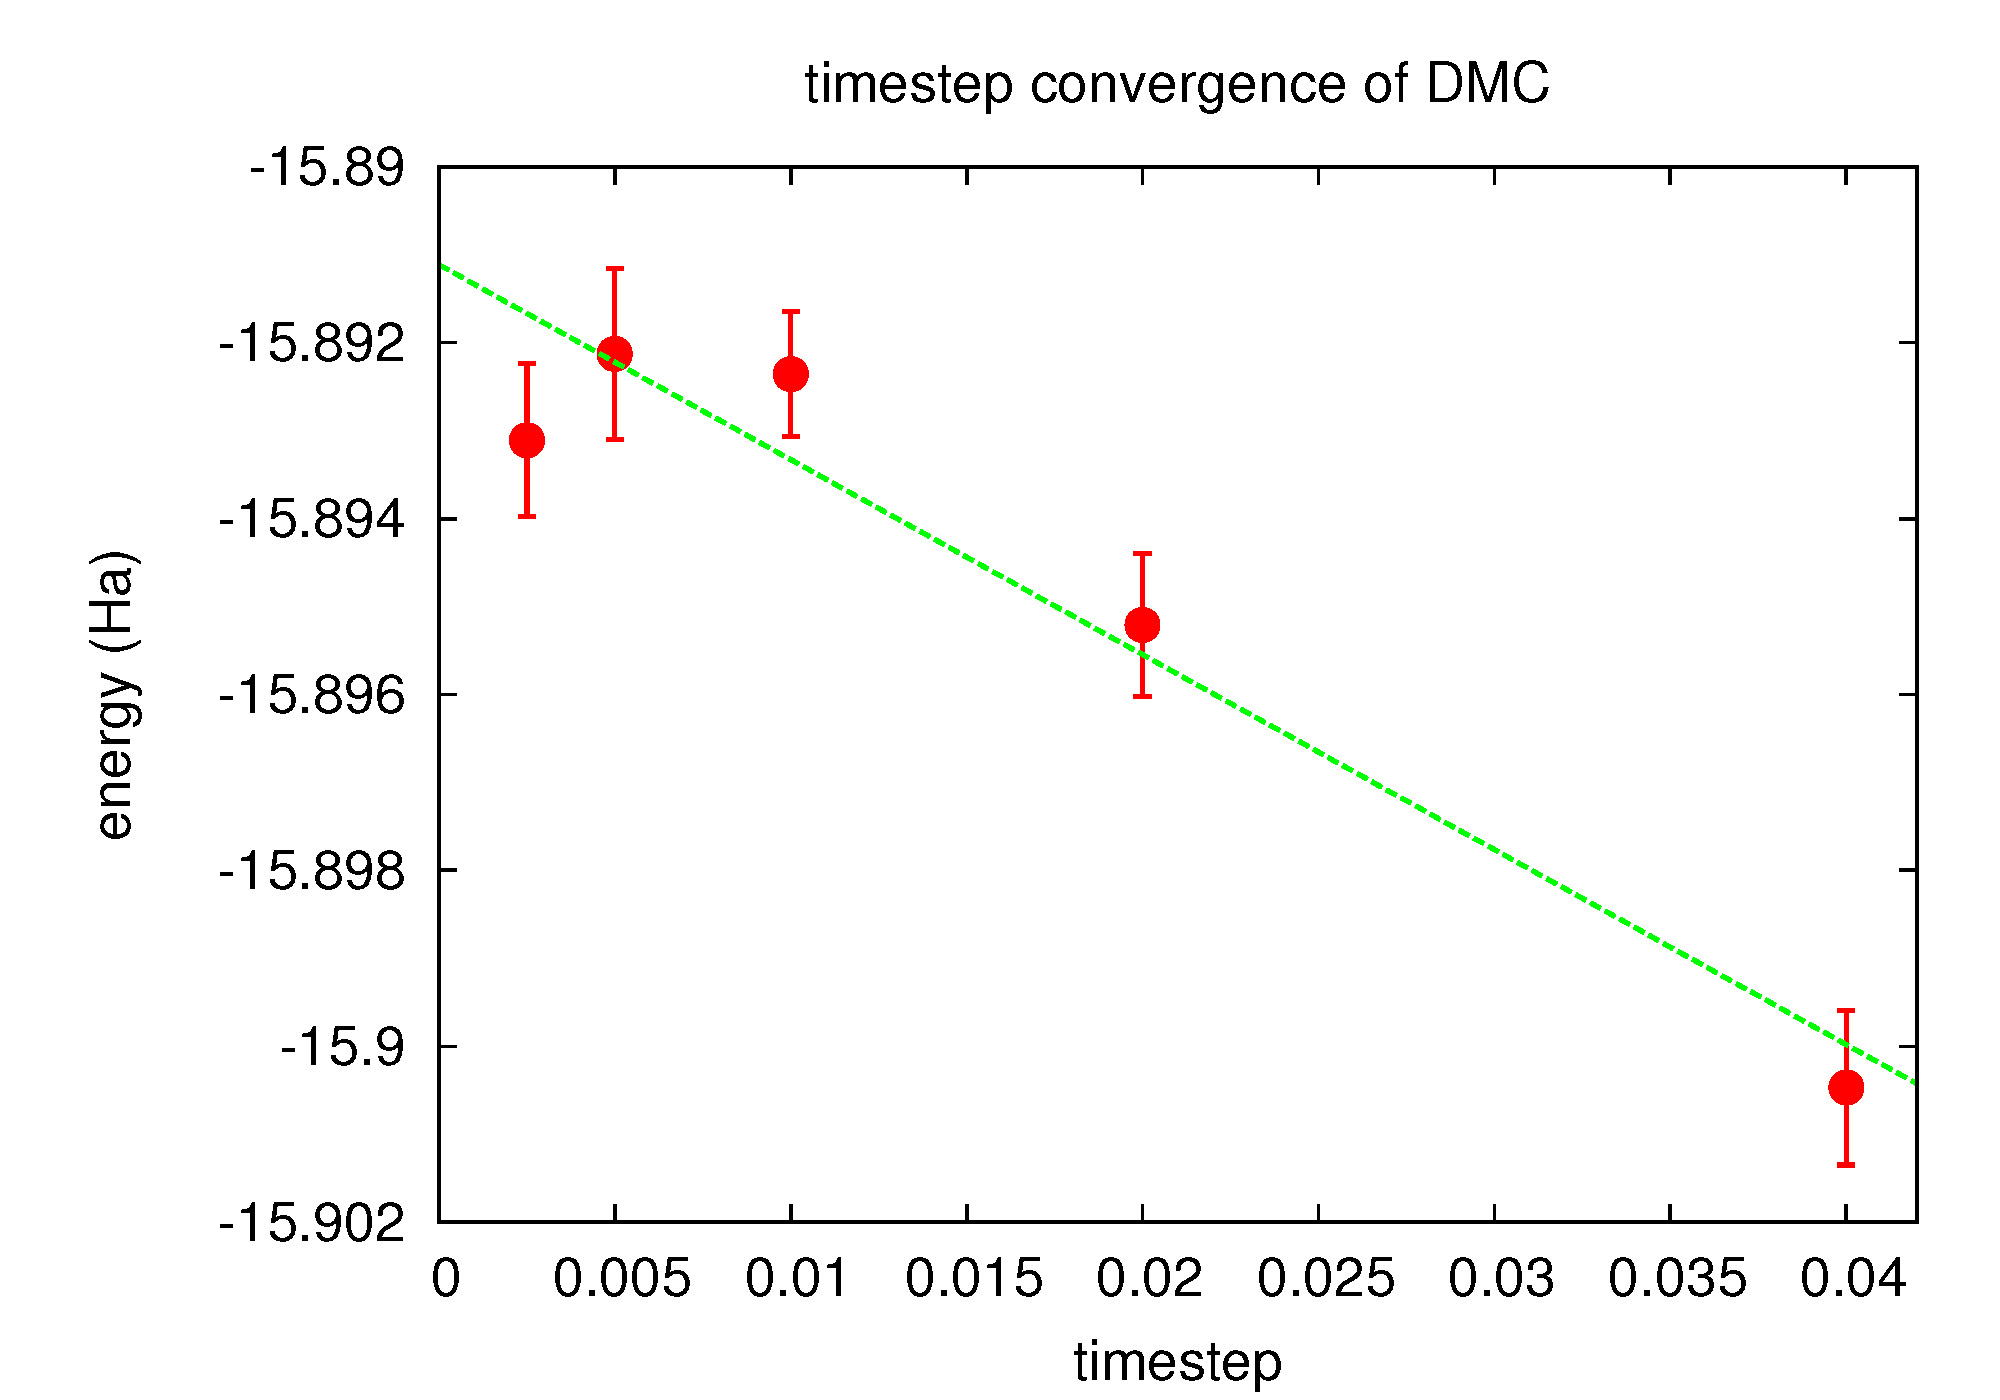
\includegraphics[trim = 0mm 0mm 0mm 0mm, clip,width=0.75\columnwidth]{./figures/lab_qmc_basics_timestep_conv.dmn}
\else
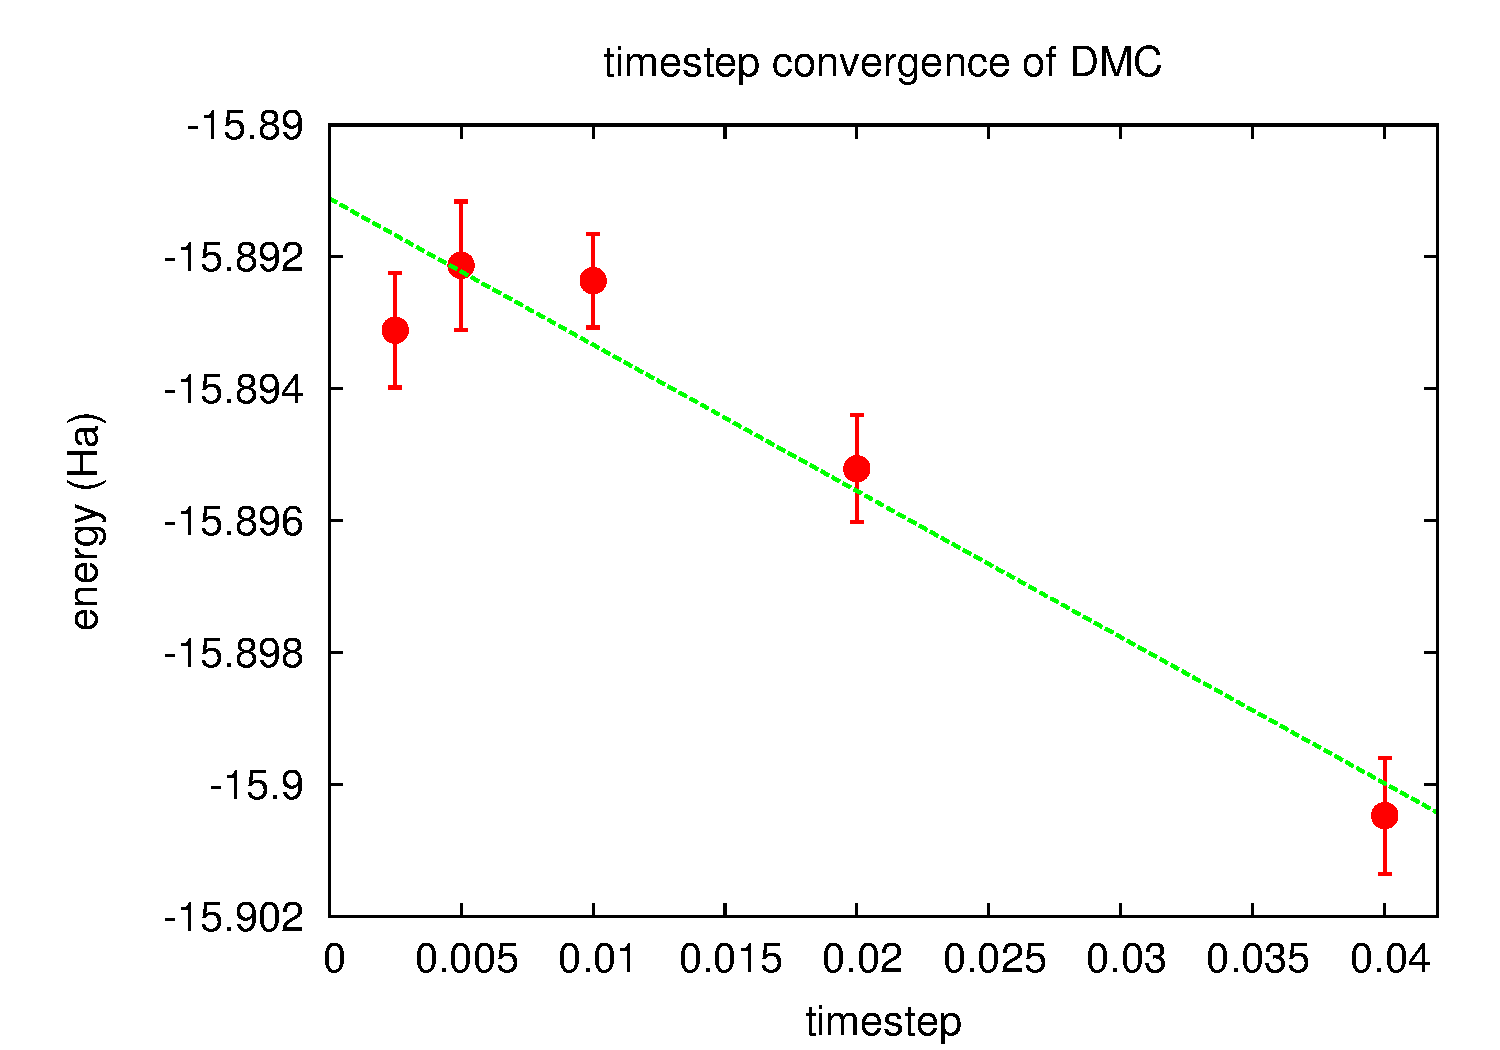
\includegraphics[trim = 0mm 0mm 0mm 0mm, clip,width=0.75\columnwidth]{./figures/lab_qmc_basics_timestep_conv.pdf}
\fi
\end{center}
\caption{Linear fit to DMC timestep data from \ishell{PlotTstepConv.pl}.}
\label{fig:timestep_conv}
\end{figure}


\vspace{1cm}
\begin{flushleft}
\textbf{\underline{Questions and Exercises}}
\end{flushleft}
\begin{enumerate}
  \item{What is the $\tau\rightarrow 0$ extrapolated value for the total energy?}
  \item{What is the maximum timestep you should use if you want to calculate the total energy to an accuracy of $0.05$ eV?  For convenience, $1~\textrm{Ha}=27.2113846~\textrm{eV}$.}
  \item{What is the acceptance ratio for this (bias$<0.05$ eV) run?  Does it follow the rule of thumb for sensible DMC (acceptance ratio $>99$\%) ?}
  \item{Check the fluctuations in the walker population (\ishell{qmca -t -q nw O.q0.dmc*dmc.dat --noac}).  Does the population seem to be stable?}
  \item{(Optional) Study population control bias for the oxygen atom.  Select a few population sizes \labsw{}{(use multiples of 512 to fit cleanly on a single Vesta partition)}.  Copy \ishell{O.q0.dmc.in.xml} to a new file and remove all but one DMC run (select a single timestep).  Make one copy of the new file for each population, set ``\ishell{samples}'', and choose a unique \ishell{id} in \ishell{<project/>}.  \labsw{}{Run one job at a time to avoid crowding the lab allocation.}  Use \ishell{qmca} to study the dependence of the DMC total energy on the walker population.  How large is the bias compared to timestep error?  What bias is incurred by following the ``rule of thumb'' of a couple thousand walkers?  Will population control bias generally be an issue for production runs on modern parallel machines?}
\end{enumerate}


\section{DMC timestep extrapolation II: O atom ionization potential}
In this section, we will repeat the calculations of the prior two sections (optimization, timestep extrapolation) for the $+1$ charge state of the oxygen atom.  Comparing the resulting 1st ionization potential (IP) with experimental data will complete our first test of the BFD oxygen pseudopotential.  In actual practice, higher IP's could also be tested prior to performing production runs.

Obtaining the timestep extrapolated DMC total energy for ionized oxygen should take much less (human) time than for the neutral case.  For convenience, the necessary steps are briefly summarized below.
\begin{enumerate}
  \item{Obtain DFT orbitals with Quantum ESPRESSO}
  \begin{enumerate}
    \item{Copy the DFT input (\ishell{O.q0.dft.in}) to \ishell{O.q1.dft.in}}
    \item{Edit \ishell{O.q1.dft.in} to match the +1 charge state of the oxygen atom}
    \begin{lstlisting}[style=espresso]
     ...
     prefix            = 'O.q1'
     ...
     tot_charge        = 1
     tot_magnetization = 3
     ...
    \end{lstlisting}
  \item{Perform the DFT run: \ifws\ishell{mpirun -np 4 pw.x -input O.q1.dft.in >&O.q1.dft.out&}
      \else\ishell{jobrun_vesta pw.x O.q1.dft.in}\fi}
  \end{enumerate}

  \item{Convert the orbitals to ESHDF format}
  \begin{enumerate}
    \item{Copy the pw2qmcpack input (\ishell{O.q0.p2q.in}) to \ishell{O.q1.p2q.in}}
    \item{Edit \ishell{O.q1.p2q.in} to match the file prefix used in DFT}
    \begin{verbatim}
     ...
     prefix = 'O.q1'
     ...
    \end{verbatim}
    \item{Perform the orbital conversion run: \ifws\ishell{mpirun -np 1 pw2qmcpack.x<O.q1.p2q.in>&O.q1.p2q.out&}\else\ishell{jobrun_vesta pw2qmcpack.x O.q1.p2q.in}\fi}
  \end{enumerate}

  \item{Optimize the Jastrow factor with QMCPACK}
  \begin{enumerate}
    \item{Copy the optimization input (\ishell{O.q0.opt.in.xml}) to \ishell{O.q1.opt.in.xml}}
    \item{Edit \ishell{O.q1.opt.in.xml} to match the file prefix used in DFT}
    \begin{lstlisting}[style=QMCPXML]
     ...
     <project id="O.q1.opt" series="0">
     ...
     <include href="O.q1.ptcl.xml"/>
     ...
     <include href="O.q1.wfs.xml"/>
     ...
    \end{lstlisting}
    \item{Edit the particle XML file (O.q1.ptcl.xml) to have open boundary conditions}
    \begin{lstlisting}[style=QMCPXML]
      <parameter name="bconds">
        n n n 
      </parameter>
    \end{lstlisting}
    \item{Add cutoffs to the Jastrow factors in the wavefunction XML file (O.q1.wfs.xml)}
    \begin{lstlisting}[style=QMCPXML]
      ...
      <correlation speciesA="u" speciesB="u" size="8" rcut="10.0">
      ...
      <correlation speciesA="u" speciesB="d" size="8" rcut="10.0">
      ...
      <correlation elementType="O" size="8" rcut="5.0">
      ...
    \end{lstlisting}
    \item{Perform the Jastrow optimization run: \ifws\ishell{mpirun -np 4 qmcpack O.q1.opt.in.xml >&O.q1.opt.out&}\else\ishell{jobrun_vesta qmcpack O.q1.opt.in.xml}\fi}
    \item{Identify the optimal set of parameters with \ishell{qmca} (\ishell{[your opt.xml]}).}
  \end{enumerate}

  \item{DMC timestep study with QMCPACK}
  \begin{enumerate}
    \item{Copy the DMC input (\ishell{O.q0.dmc.in.xml}) to \ishell{O.q1.dmc.in.xml}}
    \item{Edit \ishell{O.q1.dmc.in.xml} to use the DFT prefix and the optimal Jastrow}
    \begin{lstlisting}[style=QMCPXML]
     ...
     <project id="O.q1.dmc" series="0">
     ...
     <include href="O.q1.ptcl.xml"/>
     ...
     <include href="[your opt.xml]"/>
     ...
    \end{lstlisting}
    \item{Perform the DMC run: \ifws\ishell{mpirun -np 4 qmcpack O.q1.dmc.in.xml >&O.q1.dmc.out&}\else\ishell{jobrun_vesta qmcpack O.q1.dmc.in.xml}\fi}
    \item{Obtain the DMC total energy extrapolated to zero timestep with \ishell{PlotTstepConv.pl}.}
  \end{enumerate}
\end{enumerate}
The process listed above, which excludes additional steps for orbital generation and conversion, can become tedious to perform by hand in production settings where many calculations are often required.  For this reason automation tools are introduced for calculations involving the oxygen dimer in section \ref{sec:dimer_automation} of the lab.  

\vspace{1cm}
\begin{flushleft}
\textbf{\underline{Questions and Exercises}}
\end{flushleft}
\begin{enumerate}
  \item{What is the $\tau\rightarrow 0$ extrapolated DMC value for the 1st ionization potential of oxygen?}
  \item{How does the extrapolated value compare to the experimental IP?  Go to\newline \href{http://physics.nist.gov/PhysRefData/ASD/ionEnergy.html}{http://physics.nist.gov/PhysRefData/ASD/ionEnergy.html} and enter ``\ishell{O I}'' in the box labeled ``\ishell{Spectra}'' and click on the ``\ishell{Retrieve Data}'' button.  
%For comparison the LDA value is $12.25$ eV.
}
  \item{What can we conclude about the accuracy of the pseudopotential?  What factors complicate this assessment?}
  \item{Explore the sensitivity of the IP to the choice of timestep.  Type ``\ishell{./ip_conv.py}'' to view three timestep extrapolation plots: two for the $q=0,1$ total energies and one for the IP.  Is the IP more, less, or similarly sensitive to timestep than the total energy?}
  \item{What is the maximum timestep you should use if you want to calculate the ionization potential to an accuracy of $0.05$ eV?  What factor of cpu time is saved by assessing timestep convergence on the IP (a total energy difference) vs. a single total energy?}
  \item{Are the acceptance ratio and population fluctuations reasonable for the $q=1$ calculations?}
\end{enumerate}




\section{DMC workflow automation with Nexus}
Production QMC projects are often composed of many similar workflows.  The simplest of these is a single DMC calculation involving four different compute jobs:
\begin{enumerate}
  \item{Orbital generation via Quantum ESPRESSO or GAMESS.}
  \item{Conversion of orbital data via \ishell{pw2qmcpack.x} or \ishell{convert4qmc}.}
  \item{Optimization of Jastrow factors via QMCPACK.}
  \item{DMC calculation via QMCPACK.}
\end{enumerate}
Simulation workflows quickly become more complex with increasing costs in terms of human time for the researcher.  Automation tools can decrease both human time and error if used well.

The set of automation tools we will be using is known as Nexus \cite{Krogel2016nexus}, which is distributed with QMCPACK.  Nexus is capable of generating input files, submitting and monitoring compute jobs, passing data between simulations (such as relaxed structures, orbital files, optimized Jastrow parameters, etc.), and data analysis.  The user interface to Nexus is through a set of functions defined in the Python programming language.  User scripts that execute simple workflows resemble input files and do not require programming experience.  More complex workflows require only basic programming constructs (\emph{e.g.} for loops and if statements).  Nexus input files/scripts should be easier to navigate than QMCPACK input files and more efficient than submitting all the jobs by hand.

Nexus is driven by simple user-defined scripts that resemble keyword-driven input files.  An example Nexus input file that performs a single VMC calculation (with pre-generated orbitals) is shown below.  Take a moment to read it over and especially note the comments (prefixed with ``\ishell{\#}'') explaining most of the contents.  If the input syntax is unclear you may want to consult portions of appendix \ref{app:python_basics}, which gives a condensed summary of Python constructs.  An additional example and details about the inner workings of Nexus can be found in the reference publication \cite{Krogel2016nexus}. 

%For more information about the functionality and effective use of Nexus, consult \ishell{docs/Nexus.pdf}.  

%More information can be found in the user guide distributed with QMCPACK, although examples in this lab series and \ishell{Nexus.pdf} are more up to date (if \ishell{qmcpack} is the location of your QMCPACK distribution, the user guide can be found at \ishell{qmcpack/nexus/documentation/nexus\_user\_guide.pdf}).

\ifws
\begin{lstlisting}[style=Python]
#! /usr/bin/env python

# import Nexus functions
from nexus import settings,job,get_machine,run_project 
from nexus import generate_physical_system
from nexus import generate_qmcpack,vmc

settings(                             # Nexus settings
    pseudo_dir    = './pseudopotentials', # location of PP files
    runs          = '',                   # root directory for simulations
    results       = '',                   # root directory for simulation results
    status_only   = 0,                    # show simulation status, then exit
    generate_only = 0,                    # generate input files, then exit
    sleep         = 3,                    # seconds between checks on sim. progress
    machine       = 'ws4',                # workstation with 4 cores
    ) 

qmcjob = job(                         # specify job parameters
    cores   = 4,                          # use 4 MPI tasks
    threads = 1,                          # 1 OpenMP thread per node
    app     = 'qmcpack'                   # use QMCPACK executable (assumed in PATH)
    )

qmc_calcs = [                         # list QMC calculation methods
    vmc(                                  #   VMC
        walkers     =   1,                #     1 walker
        warmupsteps =  50,                #    50 MC steps for warmup
        blocks      = 200,                #   200 blocks
        steps       =  10,                #    10 steps per block
        timestep    =  .4                 #   0.4 1/Ha timestep
        )]

dimer = generate_physical_system(     # make a dimer system
    type       = 'dimer',                 # system type is dimer
    dimer      = ('O','O'),               # dimer is two oxygen atoms
    separation = 1.2074,                  # separated by 1.2074 Angstrom
    Lbox       = 15.0,                    # simulation box is 15 Angstrom 
    units      = 'A',                     # Angstrom is dist. unit
    net_spin   = 2,                       # nup-ndown is 2
    O          = 6                        # pseudo-oxygen has 6 valence el.
    )

qmc = generate_qmcpack(                # make a qmcpack simulation 
    identifier   = 'example',             # prefix files with 'example'
    path         = 'scale_1.0',           # run in ./scale_1.0 directory
    system       = dimer,                 # run the dimer system
    job          = qmcjob,                # set job parameters
    input_type   = 'basic',               # basic qmcpack inputs given below    
    pseudos      = ['O.BFD.xml'],         # list of PP's to use
    orbitals_h5  = 'O2.pwscf.h5',         # file with orbitals from DFT
    bconds       = 'nnn',                 # open boundary conditions
    jastrows     = [],                    # no jastrow factors
    calculations = qmc_calcs              # QMC calculations to perform
    )
                       
run_project(qmc)                       # write input file and submit job
\end{lstlisting}

\else

\begin{lstlisting}[style=Python]
#! /usr/bin/env python

# import Nexus functions
from nexus import settings,job,get_machine,run_project 
from nexus import generate_physical_system
from nexus import generate_qmcpack,vmc

settings(                             # Nexus settings
    pseudo_dir    = './pseudopotentials', # location of PP files
    runs          = '',                   # root directory for simulations
    results       = '',                   # root directory for simulation results
    status_only   = 0,                    # show simulation status, then exit
    generate_only = 0,                    # generate input files, then exit
    sleep         = 3,                    # seconds between checks on sim. progress
    machine       = 'vesta',              # name of local machine
    account       = 'QMCPACK-Training'    # charge account for cpu time
    ) 

vesta = get_machine('vesta')          # allow max of one job at a time (lab only)
vesta.queue_size = 1

qmcjob = job(                         # specify job parameters
    nodes   = 32,                         # use 32 Vesta nodes
    threads = 16,                         # 16 OpenMP threads per node (32 MPI tasks)
    hours   = 1,                          # wallclock limit of 1 hour
                                          # use QMCPACK executable
    app     = '/soft/applications/qmcpack/Binaries/qmcpack'
    )

qmc_calcs = [                         # list QMC calculation methods
    vmc(                                  #   VMC
        walkers     =   1,                #     1 walker
        warmupsteps =  50,                #    50 MC steps for warmup
        blocks      = 200,                #   200 blocks
        steps       =  10,                #    10 steps per block
        timestep    =  .4                 #   0.4 1/Ha timestep
        )]

dimer = generate_physical_system(     # make a dimer system
    type       = 'dimer',                 # system type is dimer
    dimer      = ('O','O'),               # dimer is two oxygen atoms
    separation = 1.2074,                  # separated by 1.2074 Angstrom
    Lbox       = 15.0,                    # simulation box is 15 Angstrom 
    units      = 'A',                     # Angstrom is dist. unit
    net_spin   = 2,                       # nup-ndown is 2
    O          = 6                        # pseudo-oxygen has 6 valence el.
    )

qmc = generate_qmcpack(                # make a qmcpack simulation 
    identifier   = 'example',             # prefix files with 'example'
    path         = 'scale_1.0',           # run in ./scale_1.0 directory
    system       = dimer,                 # run the dimer system
    job          = qmcjob,                # set job parameters
    input_type   = 'basic',               # basic qmcpack inputs given below    
    pseudos      = ['O.BFD.xml'],         # list of PP's to use
    orbitals_h5  = 'O2.pwscf.h5',         # file with orbitals from DFT
    bconds       = 'nnn',                 # open boundary conditions
    jastrows     = [],                    # no jastrow factors
    calculations = qmc_calcs              # QMC calculations to perform
    )
                       
run_project(qmc)                       # write input file and submit job
\end{lstlisting}
\fi





\section{Automated binding curve of the oxygen dimer}
\label{sec:dimer_automation}
In this section we will use Nexus to calculate the DMC total energy of the oxygen dimer over a series of bond lengths.  The equilibrium bond length and binding energy of the dimer will be determined by performing a polynomial fit to the data (Morse potential fits should be preferred in production tests).  Comparing these values with corresponding experimental data provides a second test of the BFD pseudopotential for oxygen.

Enter the \ishell{oxygen\_dimer} directory.  Copy your BFD pseudopotential from the atom runs into \ishell{oxygen\_dimer/pseudopotentials} (be sure to move both files: \ishell{.upf} and \ishell{.xml}).  Open \ishell{O\_dimer.py} with a text editor.  The overall format is similar to the example file shown in the last section.  
%The header material, including Nexus imports, settings, and the job parameters for QMC are identical.  
The main difference is that a full workflow of runs (DFT orbital generation, orbital conversion, optimization and DMC) are being performed rather than a single VMC run.  


%Following the job parameters, inputs for the optimization method are given.  The keywords should all be familiar from the QMCPACK XML input files you used previously:
%\begin{lstlisting}
%linopt1 = linear(
%    energy               = 0.0,
%    unreweightedvariance = 1.0,
%    reweightedvariance   = 0.0,
%    timestep             = 0.4,
%    samples              = 10240, 
%    warmupsteps          = 50,
%    blocks               = 200,
%    substeps             = 1,
%    nonlocalpp           = True,
%    usebuffer            = True,
%    walkers              = 1,
%    minwalkers           = 0.5,
%    maxweight            = 1e9,
%    usedrift             = True,
%    minmethod            = 'quartic',
%    beta                 = 0.025,
%    exp0                 = -16,
%    bigchange            = 15.0,
%    alloweddifference    = 1e-4,
%    stepsize             = 0.2,
%    stabilizerscale      = 1.0,
%    nstabilizers         = 3
%    )
%\end{lstlisting}
%
%%\hide{
%\noindent
%Requesting multiple loop's with different numbers of samples is more compact than in XML:
%\begin{lstlisting}
%linopt1 = ...
%
%linopt2 = linopt1.copy()  
%linopt2.samples = 61440 # opt w/ 61440 samples
%
%opt_calcs = [loop(max=4,qmc=linopt1), # loops over opt's
%             loop(max=8,qmc=linopt2)]
%\end{lstlisting}
%%}
%
%\noindent
%The VMC/DMC method inputs should also look familiar:
%\begin{lstlisting}
%qmc_calcs = [
%    vmc(
%        walkers     =   1,
%        warmupsteps =  30,
%        blocks      =  20,
%        steps       =  10,
%        substeps    =   2,
%        timestep    =  .4,
%        samples     = 2048
%        ),
%    dmc(
%        warmupsteps   = 100, 
%        blocks        = 400,
%        steps         =  32,
%        timestep      = 0.01,
%        nonlocalmoves = True
%        )
%    ]
%\end{lstlisting}


As in the example in the last section, the oxygen dimer is generated with the \ishell{generate\_physical\_system} function:
\begin{lstlisting}[style=Python]
dimer = generate_physical_system(
    type       = 'dimer',
    dimer      = ('O','O'),
    separation = 1.2074*scale,
    Lbox       = 10.0,
    units      = 'A',
    net_spin   = 2,
    O          = 6
    )
\end{lstlisting}
\noindent
Similar syntax can be used to generate crystal structures or to specify systems with arbitrary atomic configurations and simulation cells.  Notice that a ``\ishell{scale}'' variable has been introduced to stretch or compress the dimer.  

Next, objects representing a Quantum ESPRESSO (PWSCF) run and subsequent orbital conversion step are constructed with respective \ishell{generate\_*} functions:
\begin{lstlisting}[style=Python]
dft = generate_pwscf(
    identifier   = 'dft',
    ...
    input_dft    = 'lda',
    ...
    )
sims.append(dft)

# describe orbital conversion run                                                                    
p2q = generate_pw2qmcpack(
    identifier   = 'p2q',
    ...
    dependencies = (dft,'orbitals'),
    )
sims.append(p2q)
\end{lstlisting}
Note the \ishell{dependencies} keyword.  This keyword is used to construct workflows out of otherwise separate runs.  In this case, the dependency indicates that the orbital conversion run must wait for the DFT to finish prior to starting.

Objects representing QMCPACK simulations are then constructed with the \ishell{generate\_qmcpack} function:
\begin{lstlisting}[style=Python]
opt = generate_qmcpack(
    identifier   = 'opt',
    ...
    jastrows     = [('J1','bspline',8,5.0), 
                    ('J2','bspline',8,10.0)],
    calculations = [
        loop(max=12,
             qmc=linear(
                energy               = 0.0,
                unreweightedvariance = 1.0,
                reweightedvariance   = 0.0,
                timestep             = 0.3,
                samples              = 61440,
                warmupsteps          = 50,
                blocks               = 200,
                substeps             = 1,
                nonlocalpp           = True,
                usebuffer            = True,
                walkers              = 1,
                minwalkers           = 0.5,
                maxweight            = 1e9,
                usedrift             = False,
                minmethod            = 'quartic',
                beta                 = 0.025,
                exp0                 = -16,
                bigchange            = 15.0,
                alloweddifference    = 1e-4,
                stepsize             = 0.2,
                stabilizerscale      = 1.0,
                nstabilizers         = 3,
                )
             )
        ],
    dependencies = (p2q,'orbitals'),
    )
sims.append(opt)

qmc = generate_qmcpack(
    identifier   = 'qmc',
    ...
    jastrows     = [],            
    calculations = [
        vmc(
            walkers     =   1,
            warmupsteps =  30,
            blocks      =  20,
            steps       =  10,
            substeps    =   2,
            timestep    =  .4,
            samples     = 2048
            ),
        dmc(
            warmupsteps   = 100,
            blocks        = 400,
            steps         =  32,
            timestep      = 0.01,
            nonlocalmoves = True,
            )
        ],
    dependencies = [(p2q,'orbitals'),(opt,'jastrow')],
    )
sims.append(qmc)
\end{lstlisting}
\noindent
Shared details such as the run directory, job, pseudopotentials, and orbital file have been omitted (\ishell{...}).  The ``\ishell{opt}'' run will optimize a 1-body B-spline Jastrow with 8 knots having a cutoff of 5.0 Bohr and a B-spline Jastrow (for up-up and up-down correlations) with 8 knots and cutoffs of 10.0 Bohr.  The Jastrow list for the DMC run is empty and the usage of \ishell{dependencies} above indicates that the DMC run depends on the optimization run for the Jastrow factor.  Nexus will submit the ``\ishell{opt}'' run first and upon completion it will scan the output, select the optimal set of parameters, pass the Jastrow information to the ``\ishell{qmc}'' run and then submit the DMC job.  Independent job workflows are submitted in parallel when permitted \labsw{}{(we have explicitly limited this for this lab by setting \ishell{queue\_size=2} for Vesta)}.  No input files are written or job submissions made until the ``\ishell{run\_project}'' function is reached:
\begin{lstlisting}[style=Python]
run_project(sims)
\end{lstlisting}
\noindent
All of the simulations objects have been collected into a list (\ishell{sims}) for submission.

As written, \ishell{O\_dimer.py} will only perform calculations at the equilibrium separation distance of 1.2074 Angstrom, since the list of scaling factors (representing stretching or compressing the dimer) only contains one value (\ishell{scales = [1.00]}).  Modify the file now to perform DMC calculations across a range of separation distances with each DMC run using the Jastrow factor optimized at the equilibrium separation distance.  Specifically, you will want to change the list of scaling factors to include both compression (\ishell{scale<1.0}) and stretch (\ishell{scale>1.0}): 
\begin{lstlisting}[style=Python]
scales = [1.00,0.90,0.95,1.05,1.10]
\end{lstlisting}
\noindent
Note that ``\ishell{1.00}'' is left in front because we are going to optimize the Jastrow factor first at the equilibrium separation and reuse this Jastrow factor for all other separation distances.  This procedure is used because it can reduce variations in localization errors (due to pseudopotentials in DMC) along the binding curve. 

Change the ``\ishell{status\_only}'' parameter in the ``\ishell{settings}'' function to \ishell{1} and type ``./O\_dimer.py'' at the command line.  This will print the status of all simulations:
\begin{shade}
Project starting 
  checking for file collisions 
  loading cascade images 
    cascade 0 checking in 
    cascade 10 checking in 
    cascade 4 checking in 
    cascade 13 checking in 
    cascade 7 checking in 
  checking cascade dependencies 
    all simulation dependencies satisfied 
  
  cascade status 
    setup, sent_files, submitted, finished, got_output, analyzed 
    000000  dft     ./scale_1.0 
    000000  p2q     ./scale_1.0 
    000000  opt     ./scale_1.0 
    000000  qmc     ./scale_1.0 
    000000  dft     ./scale_0.9 
    000000  p2q     ./scale_0.9 
    000000  qmc     ./scale_0.9 
    000000  dft     ./scale_0.95 
    000000  p2q     ./scale_0.95 
    000000  qmc     ./scale_0.95 
    000000  dft     ./scale_1.05 
    000000  p2q     ./scale_1.05 
    000000  qmc     ./scale_1.05 
    000000  dft     ./scale_1.1 
    000000  p2q     ./scale_1.1 
    000000  qmc     ./scale_1.1 
    setup, sent_files, submitted, finished, got_output, analyzed 
\end{shade}
\noindent
In this case, five simulation ``cascades'' (workflows) have been identified, each one starting and ending with ``\ishell{dft}'' and ``\ishell{qmc}'' runs, respectively.  The six status flags (\ishell{setup}, \ishell{sent\_files}, \ishell{submitted}, \ishell{finished}, \ishell{got\_output}, \ishell{analyzed}) each show \ishell{0}, indicating that no work has been done yet.  

Now change ``\ishell{status\_only}'' back to \ishell{0}, set ``\ishell{generate\_only}'' to \ishell{1}, and run \ishell{O\_dimer.py} again.  This will perform a dry-run of all simulations.  The dry-run should finish in about 20 seconds:
\ifws
\begin{shade}
Project starting 
  checking for file collisions 
  loading cascade images 
    cascade 0 checking in 
    cascade 10 checking in 
    cascade 4 checking in 
    cascade 13 checking in 
    cascade 7 checking in 
  checking cascade dependencies 
    all simulation dependencies satisfied 
  
  starting runs:
  ~~~~~~~~~~~~~~~~~~~~~~~~~~~~~~ 
  poll 0  memory 91.03 MB 
    Entering ./scale_1.0 0 
      writing input files  0 dft 
    Entering ./scale_1.0 0 
      sending required files  0 dft 
      submitting job  0 dft 
  ...
  poll 1  memory 91.10 MB 
  ...
    Entering ./scale_1.0 0 
      Would have executed:  
        export OMP_NUM_THREADS=1
        mpirun -np 4 pw.x -input dft.in 

  poll 2  memory 91.10 MB 
    Entering ./scale_1.0 0 
      copying results  0 dft 
    Entering ./scale_1.0 0 
      analyzing  0 dft 
  ...
  poll 3  memory 91.10 MB 
    Entering ./scale_1.0 1 
      writing input files  1 p2q 
    Entering ./scale_1.0 1 
      sending required files  1 p2q 
      submitting job  1 p2q 
  ...
    Entering ./scale_1.0 1 
      Would have executed:  
        export OMP_NUM_THREADS=1
        mpirun -np 1 pw2qmcpack.x<p2q.in 

  poll 4  memory 91.10 MB 
    Entering ./scale_1.0 1 
      copying results  1 p2q 
    Entering ./scale_1.0 1 
      analyzing  1 p2q 
  ...
  poll 5  memory 91.10 MB 
    Entering ./scale_1.0 2 
      writing input files  2 opt 
    Entering ./scale_1.0 2 
      sending required files  2 opt 
      submitting job  2 opt 
  ...
    Entering ./scale_1.0 2 
      Would have executed:  
        export OMP_NUM_THREADS=1
        mpirun -np 4 qmcpack opt.in.xml 

  poll 6  memory 91.16 MB 
    Entering ./scale_1.0 2 
      copying results  2 opt 
    Entering ./scale_1.0 2 
      analyzing  2 opt 
  ...
  poll 7  memory 93.00 MB 
    Entering ./scale_1.0 3 
      writing input files  3 qmc 
    Entering ./scale_1.0 3 
      sending required files  3 qmc 
      submitting job  3 qmc 
  ...
    Entering ./scale_1.0 3 
      Would have executed:  
        export OMP_NUM_THREADS=1
        mpirun -np 4 qmcpack qmc.in.xml 
  ...
  poll 17  memory 93.06 MB 
Project finished
\end{shade}
\else
\begin{shade}
Project starting 
  checking for file collisions 
  loading cascade images 
    cascade 0 checking in 
    cascade 10 checking in 
    cascade 4 checking in 
    cascade 13 checking in 
    cascade 7 checking in 
  checking cascade dependencies 
    all simulation dependencies satisfied 
  
  starting runs:
  ~~~~~~~~~~~~~~~~~~~~~~~~~~~~~~ 
  poll 0  memory 91.03 MB 
    Entering ./scale_1.0 0 
      writing input files  0 dft 
    Entering ./scale_1.0 0 
      sending required files  0 dft 
      submitting job  0 dft 
  ...
  poll 1  memory 91.10 MB 
  ...
    Entering ./scale_1.0 1 
      Would have executed:  qsub --mode script --env BG_SHAREDMEMSIZE=32 dft.qsub.in 

  poll 2  memory 91.10 MB 
    Entering ./scale_1.0 0 
      copying results  0 dft 
    Entering ./scale_1.0 0 
      analyzing  0 dft 
  ...
  poll 3  memory 91.10 MB 
    Entering ./scale_1.0 1 
      writing input files  1 p2q 
    Entering ./scale_1.0 1 
      sending required files  1 p2q 
      submitting job  1 p2q 
  ...
    Entering ./scale_1.0 2 
      Would have executed:  qsub --mode script --env BG_SHAREDMEMSIZE=32 p2q.qsub.in 

  poll 4  memory 91.10 MB 
    Entering ./scale_1.0 1 
      copying results  1 p2q 
    Entering ./scale_1.0 1 
      analyzing  1 p2q
  ... 

  poll 5  memory 91.10 MB 
    Entering ./scale_1.0 2 
      writing input files  2 opt 
    Entering ./scale_1.0 2 
      sending required files  2 opt 
      submitting job  2 opt 
  ...
    Entering ./scale_1.0 3 
      Would have executed:  qsub --mode script --env BG_SHAREDMEMSIZE=32 opt.qsub.in 

  poll 6  memory 91.16 MB 
    Entering ./scale_1.0 2 
      copying results  2 opt 
    Entering ./scale_1.0 2 
      analyzing  2 opt 
  ...
  poll 7  memory 93.00 MB 
    Entering ./scale_1.0 3 
      writing input files  3 qmc 
    Entering ./scale_1.0 3 
      sending required files  3 qmc 
      submitting job  3 qmc 
  ...
    Entering ./scale_1.0 4 
      Would have executed:  qsub --mode script --env BG_SHAREDMEMSIZE=32 qmc.qsub.in 
  ...

  poll 17  memory 93.00 MB 
Project finished
\end{shade}
\fi

\noindent
Nexus polls the simulation status every 3 seconds and sleeps in between.  The ``scale\_*'' directories should now contain several files:
\ifws
\begin{shade}
scale_1.0
   dft.in
   O.BFD.upf
   O.BFD.xml
   opt.in.xml
   p2q.in
   pwscf_output
   qmc.in.xml
   sim_dft/
       analyzer.p
       input.p
       sim.p
   sim_opt/
       analyzer.p
       input.p
       sim.p
   sim_p2q/
       analyzer.p
       input.p
       sim.p
   sim_qmc/
       analyzer.p
       input.p
       sim.p
\end{shade}
\else
\begin{shade}
scale_1.0
   dft.in
   dft.qsub.in
   O.BFD.upf
   O.BFD.xml
   opt.in.xml
   opt.qsub.in
   p2q.in
   p2q.qsub.in
   pwscf_output
   qmc.in.xml
   qmc.qsub.in
   sim_dft/
       analyzer.p
       input.p
       sim.p
   sim_opt/
       analyzer.p
       input.p
       sim.p
   sim_p2q/
       analyzer.p
       input.p
       sim.p
   sim_qmc/
       analyzer.p
       input.p
       sim.p
\end{shade}
\fi
\noindent
Take a minute to inspect the generated input (\ishell{dft.in}, \ishell{p2q.in}, \ishell{opt.in.xml}, \ishell{qmc.in.xml}) \labsw{}{and submission (\ishell{dft.qsub.in}, \ishell{p2q.qsub.in}, \ishell{opt.qsub.in}, \ishell{qmc.qsub.in})} files.  The pseudopotential files (\ishell{O.BFD.upf} and \ishell{O.BFD.xml}) have been copied into each local directory. Four additional directories have been created: \ishell{sim\_dft},  \ishell{sim\_p2q}, \ishell{sim\_opt} and \ishell{sim\_qmc}.  The \ishell{sim.p} files in each directory contain the current status of each simulation.  If you run \ishell{O\_dimer.py} again, it should not attempt to rerun any of the simulations:   
\begin{shade}
Project starting 
  checking for file collisions 
  loading cascade images 
    cascade 0 checking in 
    cascade 10 checking in 
    cascade 4 checking in 
    cascade 13 checking in 
    cascade 7 checking in 
  checking cascade dependencies 
    all simulation dependencies satisfied 
  
  starting runs:
  ~~~~~~~~~~~~~~~~~~~~~~~~~~~~~~ 
  poll 0  memory 64.25 MB 
Project finished
\end{shade}
\noindent
This way one can continue to add to the \ishell{O\_dimer.py} file (\emph{e.g.} adding more separation distances) without worrying about duplicate job submissions.

Let's actually submit the jobs in the dimer workflow now.  Reset the state of the simulations by removing the \ishell{sim.p} files (``\ishell{rm ./scale*/sim*/sim.p}''), set ``\ishell{generate\_only}'' to \ishell{0}, and rerun \ishell{O\_dimer.py}.  It should take about 20 minutes for all the jobs to complete.  You may wish to open another terminal to monitor the progress of the individual jobs while the current terminal runs \ishell{O\_dimer.py} in the foreground.  You can begin the first exercise below once the optimization job completes.

\vspace{3cm}
\begin{flushleft}
\textbf{\underline{Questions and Exercises}}
\end{flushleft}
\begin{enumerate}
  \item{Evaluate the quality of the optimization at \ishell{scale=1.0} using the \ishell{qmca} tool.  Did the optimization succeed?  How does the variance compare with the neutral oxygen atom?  Is the wavefunction of similar quality to the atomic case?}

  \item{Evaluate the traces of the local energy and the DMC walker population for each separation distance with the \ishell{qmca} tool.  Are there any anomalies in the runs?  Is the acceptance ratio reasonable?  Is the wavefunction of similar quality across all separation distances?}

  \item{Use the \ishell{dimer\_fit.py} tool located in \ishell{oxygen\_dimer} to fit the oxygen dimer binding curve.   To get the binding energy of the dimer, we will need the DMC energy of the atom.  Before performing the fit, answer: What DMC timestep should be used for the oxygen atom results?  The tool accepts three arguments (``\ishell{./dimer_fit.py P N E Eerr}''}), \ishell{P} is the prefix of the DMC input files (should be ``\ishell{qmc}'' at this point), \ishell{N} is the order of the fit (use 2 to start), \ishell{E} and \ishell{Eerr} are your DMC total energy and error bar, respectively for the oxygen atom (in eV).  A plot of the dimer data will be displayed and text output will show the DMC equilibrium bond length and binding energy as well as experimental values.  How accurately does your fit to the DMC data reproduce the experimental values?  What factors affect the accuracy of your results? 

  \item{Refit your data with a fourth-order polynomial.  How do your predictions change with a fourth-order fit?  Is a fourth-order fit appropriate for the available data?}
 
  \item{Add new ``\ishell{scale}'' values to the list in \ishell{O\_dimer.py} that interpolate between the original set (e.g. expand to \ishell{[1.00,0.90,0.925,0.95,0.975,1.025,1.05,1.075,1.10]}).  Perform the DMC calculations and redo the fits.  How accurately does your fit to the DMC data reproduce the experimental values?  Should this pseudopotential be used in production calculations?}

  \item{(Optional) Perform optimization runs at the extremal separation distances corresponding to \ishell{scale=[0.90,1.10]}}.  Are the individually optimized wavefunctions of significantly better quality than the one imported from \ishell{scale=1.00}?  Why?  What form of Jastrow factor might give an even better improvement? 
\end{enumerate}




\section{(Optional) Running your system with QMCPACK}\label{sec:your_system}
This section covers a fairly simple route to get started on QMC calculations of an arbitrary system of interest using the Nexus workflow management system to setup input files and optionally perform the runs.  The example provided in this section uses QM Espresso (PWSCF) to generate the orbitals forming the Slater determinant part of the trial wavefunction.  PWSCF is a natural choice for solid state systems and it can be used for surface/slab and molecular systems as well, albeit at the price of describing additional vacuum space with plane waves.

To start out with, you will need pseudopotentials (PP's) for each element in your system in both the UPF (PWSCF) and FSATOM/XML (QMCPACK) formats.  A good place to start is the Burkatzki-Filippi-Dolg (BFD) pseudopotential database \newline (\href{http://www.burkatzki.com/pseudos/index.2.html}{http://www.burkatzki.com/pseudos/index.2.html}), which we have already used in our study of the oxygen atom.  The database does not contain PP's for the 4th and 5th row transition metals or any of the lanthanides or actinides.  If you need a PP that is not in the BFD database, you may need to generate and test one manually (\emph{e.g.} with OPIUM, \href{http://opium.sourceforge.net/}{http://opium.sourceforge.net/}).  Otherwise, use \ishell{ppconvert} as outlined in section \ref{sec:lqb_pseudo} to obtain PP's in the formats used by PWSCF and QMCPACK.  Enter the \ishell{your\_system} lab directory and place the converted PP's in \ishell{your\_system/pseudopotentials}.

Before performing production calculations (more than just the initial setup in this section) be sure to converge the plane wave energy cutoff in PWSCF as these PP's can be rather hard, sometimes requiring cutoffs in excess of 300 Ry.  Depending on the system under study, the amount of memory required to represent the orbitals (QMCPACK uses 3D B-splines) becomes prohibitive and one may be forced to search for softer PP's.

Beyond pseudopotentials, all that is required to get started are the atomic positions and the dimensions/shape of the simulation cell.  The Nexus file \ishell{example.py} illustrates how to setup PWSCF and QMCPACK input files by providing minimal information regarding the physical system (an 8-atom cubic cell of diamond in the example).  Most of the contents should be familiar from your experience with the automated calculations of the oxygen dimer binding curve in section \ref{sec:dimer_automation} (if you've skipped ahead you may want to skim that section for relevant information).  The most important change is the expanded description of the physical system:

\begin{lstlisting}[style=Python]
# details of your physical system (diamond conventional cell below)
my_project_name = 'diamond_vmc'   # directory to perform runs
my_dft_pps      = ['C.BFD.upf']   # pwscf pseudopotentials
my_qmc_pps      = ['C.BFD.xml']   # qmcpack pseudopotentials

#  generate your system
#    units      :  'A'/'B' for Angstrom/Bohr
#    axes       :  simulation cell axes in cartesian coordinates (a1,a2,a3)
#    elem       :  list of atoms in the system
#    pos        :  corresponding atomic positions in cartesian coordinates
#    kgrid      :  Monkhorst-Pack grid
#    kshift     :  Monkhorst-Pack shift (between 0 and 0.5)
#    net_charge :  system charge in units of e
#    net_spin   :  # of up spins - # of down spins
#    C = 4      :  (pseudo) carbon has 4 valence electrons
my_system = generate_physical_system(
    units      = 'A',
    axes       = [[ 3.57000000e+00, 0.00000000e+00, 0.00000000e+00],
                  [ 0.00000000e+00, 3.57000000e+00, 0.00000000e+00],
                  [ 0.00000000e+00, 0.00000000e+00, 3.57000000e+00]],
    elem       = ['C','C','C','C','C','C','C','C'],
    pos        = [[ 0.00000000e+00, 0.00000000e+00, 0.00000000e+00],
                  [ 8.92500000e-01, 8.92500000e-01, 8.92500000e-01],
                  [ 0.00000000e+00, 1.78500000e+00, 1.78500000e+00],
                  [ 8.92500000e-01, 2.67750000e+00, 2.67750000e+00],
                  [ 1.78500000e+00, 0.00000000e+00, 1.78500000e+00],
                  [ 2.67750000e+00, 8.92500000e-01, 2.67750000e+00],
                  [ 1.78500000e+00, 1.78500000e+00, 0.00000000e+00],
                  [ 2.67750000e+00, 2.67750000e+00, 8.92500000e-01]],
    kgrid      = (1,1,1),
    kshift     = (0,0,0),
    net_charge = 0,
    net_spin   = 0,
    C          = 4       # one line like this for each atomic species
    )

my_bconds       = 'ppp'  #  ppp/nnn for periodic/open BC's in QMC
                         #  if nnn, center atoms about (a1+a2+a3)/2
\end{lstlisting}

If you have a system you would like to try with QMC, make a copy of \ishell{example.py} and fill in the relevant information about the pseudopotentials, simulation cell axes, and atomic species/positions.  Otherwise, you can proceed with \ishell{example.py} as it is.

%The other new aspects are two additional compute jobs to generate the orbitals with PWSCF and convert them into the ESHDF format with \ishell{pw2qmcpack.x}:

%\begin{lstlisting}[style=Python]
%# scf run to generate orbitals
%scf = generate_pwscf(
%    identifier   = 'scf',
%    path         = my_project_name,
%    job          = Job(nodes=32,hours=2,app=pwscf),
%    input_type   = 'scf',
%    system       = my_system,
%    pseudos      = my_dft_pps,
%    input_dft    = 'lda', 
%    ecut         = 200,   # PW energy cutoff in Ry
%    conv_thr     = 1e-8, 
%    mixing_beta  = .7,
%    nosym        = True,
%    wf_collect   = True
%    )
%
%# conversion step to create h5 file with orbitals
%p2q = generate_pw2qmcpack(
%    identifier   = 'p2q',
%    path         = my_project_name,
%    job          = Job(cores=1,hours=2,app=pw2qmcpack),
%    write_psir   = False,
%    dependencies = (scf,'orbitals')
%    )
%\end{lstlisting}

Set ``\ishell{generate\_only}'' to \ishell{1} and type ``\ishell{./example.py}'' or similar to generate the input files.  All files will be written to ``\ishell{./diamond\_vmc}'' (``\ishell{./[my\_project\_name]}'' if you have changed ``\ishell{my\_project\_name}'' in the file).  The input files for PWSCF, pw2qmcpack, and QMCPACK are \ishell{scf.in}, \ishell{pw2qmcpack.in}, and \ishell{vmc.in.xml}, respectively.  Take some time to inspect the generated input files.  If you have questions about the file contents, or run into issues with the generation process, feel free to consult with a lab instructor.  

If desired, you can submit the runs directly with \ishell{example.py}.  To do this, first reset the Nexus simulation record by typing ``\ishell{rm ./diamond\_vmc/sim*/sim.p}'' or similar and set ``\ishell{generate\_only}'' back to \ishell{0}.  Next rerun \ishell{example.py}  (you may want to redirect the text output).  

Alternatively the runs can be submitted by hand:
\ifws
\begin{shade}
mpirun -np 4 pw.x<scf.in>&scf.out&

(wait until JOB DONE appears in scf.out)

mpirun -np 1 pw2qmcpack.x<p2q.in>&p2q.out&
\end{shade}
\else
\begin{shade}
qsub --mode script --env BG_SHAREDMEMSIZE=32 scf.qsub.in

(wait until JOB DONE appears in scf.output)

qsub --mode script --env BG_SHAREDMEMSIZE=32 p2q.qsub.in
\end{shade}
\fi
Once the conversion process has finished the orbitals should be located in the file \newline \ishell{diamond\_vmc/pwscf\_output/pwscf.pwscf.h5}.  Open \ishell{diamond\_vmc/vmc.in.xml} and replace ``\ishell{MISSING.h5}'' with ``\ishell{./pwscf\_output/pwscf.pwscf.h5}''.  Next submit the VMC run:
\ifws
\begin{shade}
mpirun -np 4 qmcpack vmc.in.xml>&vmc.out&
\end{shade}
\else
\begin{shade}
qsub --mode script --env BG_SHAREDMEMSIZE=32 vmc.qsub.in
\end{shade}
\fi
Note: If your system is large, the above process may not complete within the time frame of this lab.  Working with a stripped down (but relevant) example is a good idea for exploratory runs.

Once the runs have finished, you may want to begin exploring Jastrow optimization and DMC for your system.  Example calculations are provided at the end of \ishell{example.py} in the commented out text.



%\section{(Optional) Revisiting the oxygen atom: 3-body Jastrow \& population control bias}

%\subsection{Optimization of 3-body Jastrow factors}

%\subsection{Investigation of DMC population control bias}




% cover basic python elsewhere in the manual?  refer to Nexus user guide or websites instead?
%\hide{

\section{Appendix A: Basic Python constructs\label{app:python_basics}}
Basic Python data types (\ishell{int}, \ishell{float}, \ishell{str}, \ishell{tuple}, \ishell{list}, \ishell{array}, \ishell{dict}, \ishell{obj}) and programming constructs (\ishell{if} statements, \ishell{for} loops, functions w/ keyword arguments) are briefly overviewed below.  All examples can be executed interactively in Python.  To do this, type ``\ishell{python}'' at the command line and paste any of the shaded text below at the ``\ishell{>>>}'' prompt.  For more information about effective use of Python, consult the detailed online documentation: \href{https://docs.python.org/2/}{https://docs.python.org/2/}.

\subsubsection{Intrinsic types: \ishell{int, float, str}}
\begin{shade}
#this is a comment
i=5                     # integer
f=3.6                   # float
s='quantum/monte/carlo' # string
n=None                  # represents "nothing"

f+=1.4                  # add-assign (-,*,/ also): 5.0
2**3                    # raise to a power: 8
str(i)                  # int to string: '5'
s+'/simulations'        # joining strings: 'quantum/monte/carlo/simulations'
'i={0}'.format(i)       # format string: 'i=5'

\end{shade}

 
\subsubsection{Container types: \ishell{tuple, list, array, dict, obj}}
\begin{shade}
from numpy import array  # get array from numpy module
from generic import obj  # get obj from Nexus' generic module 

t=('A',42,56,123.0)     # tuple

l=['B',3.14,196]        # list

a=array([1,2,3])        # array

d={'a':5,'b':6}         # dict

o=obj(a=5,b=6)          # obj

                        # printing
print t                 #  ('A', 42, 56, 123.0)
print l                 #  ['B', 3.1400000000000001, 196]
print a                 #  [1 2 3]
print d                 #  {'a': 5, 'b': 6}
print o                 #    a               = 5
                        #    b               = 6

len(t),len(l),len(a),len(d),len(o) #number of elements: (4, 3, 3, 2, 2)

t[0],l[0],a[0],d['a'],o.a  #element access: ('A', 'B', 1, 5, 5)

s = array([0,1,2,3,4])  # slices: works for tuple, list, array
s[:]                    #   array([0, 1, 2, 3, 4])
s[2:]                   #   array([2, 3, 4])
s[:2]                   #   array([0, 1])
s[1:4]                  #   array([1, 2, 3])
s[0:5:2]                #   array([0, 2, 4])

                        # list operations
l2 = list(l)            #   make independent copy
l.append(4)             #   add new element: ['B', 3.14, 196, 4]
l+[5,6,7]               #   addition: ['B', 3.14, 196, 4, 5, 6, 7]
3*[0,1]                 #   multiplication:  [0, 1, 0, 1, 0, 1]

b=array([5,6,7])        # array operations
a2 = a.copy()           #   make independent copy
a+b                     #   addition: array([ 6, 8, 10])
a+3                     #   addition: array([ 4, 5, 6])
a*b                     #   multiplication: array([ 5, 12, 21])
3*a                     #   multiplication: array([3, 6, 9])

                        # dict/obj operations
d2 = d.copy()           #   make independent copy
d['c'] = 7              #   add/assign element 
d.keys()                #   get element names: ['a', 'c', 'b']
d.values()              #   get element values: [5, 7, 6]

                        # obj-specific operations
o.c = 7                 #   add/assign element
o.set(c=7,d=8)          #   add/assign multiple elements

\end{shade}
An important feature of Python to be aware of is that assignment is most often by reference, \emph{i.e.} new values are not always created.  This point is illustrated below with an \ishell{obj} instance, but it also holds for \ishell{list}, \ishell{array}, \ishell{dict}, and others.
\begin{shade}
>>> o = obj(a=5,b=6)
>>> 
>>> p=o
>>> 
>>> p.a=7
>>> 
>>> print o
  a               = 7
  b               = 6

>>> q=o.copy()
>>> 
>>> q.a=9
>>> 
>>> print o
  a               = 7
  b               = 6
\end{shade}
\noindent
Here \ishell{p} is just another name for \ishell{o}, while \ishell{q} is a fully independent copy of it.


\subsubsection{Conditional Statements: \ishell{if/elif/else}}
\begin{shade}
a = 5
if a is None:
    print 'a is None'
elif a==4:
    print 'a is 4'
elif a<=6 and a>2:
    print 'a is in the range (2,6]'
elif a<-1 or a>26:
    print 'a is not in the range [-1,26]'
elif a!=10: 
    print 'a is not 10'
else:
    print 'a is 10'
#end if

\end{shade}
The ``\ishell{\#end if}'' is not part of Python syntax, but you will see text like this throughout Nexus for clear encapsulation.

\subsubsection{Iteration: \ishell{for}}
\begin{shade}
from generic import obj

l = [1,2,3]              
m = [4,5,6]
s = 0
for i in range(len(l)):  # loop over list indices
    s += l[i] + m[i]
#end for

print s                  # s is 21

s = 0                    
for v in l:              # loop over list elements
    s += v
#end for

print s                  # s is 6

o = obj(a=5,b=6)
s = 0
for v in o:              # loop over obj elements
    s += v
#end for

print s                  # s is 11

d = {'a':5,'b':4}
for n,v in o.iteritems():# loop over name/value pairs in obj
    d[n] += v
#end for

print d                  # d is {'a': 10, 'b': 10}

\end{shade}


\subsubsection{Functions: \ishell{def}, argument syntax}
\begin{shade}
def f(a,b,c=5):          # basic function, c has a default value
    print a,b,c
#end def f

f(1,b=2)                 # prints: 1 2 5


def f(*args,**kwargs):   # general function, returns nothing
    print args           #     args: tuple of positional arguments
    print kwargs         #   kwargs: dict of keyword arguments
#end def f

f('s',(1,2),a=3,b='t')   # 2 pos., 2 kw. args, prints:
                         #   ('s', (1, 2))
                         #   {'a': 3, 'b': 't'}

l = [0,1,2]
f(*l,a=6)                # pos. args from list, 1 kw. arg, prints:
                         #   (0, 1, 2)
                         #   {'a': 6}
o = obj(a=5,b=6)
f(*l,**o)                # pos./kw. args from list/obj, prints:
                         #   (0, 1, 2)
                         #   {'a': 5, 'b': 6}

f(                       # indented kw. args, prints
    blocks   = 200,      #   () 
    steps    = 10,       #   {'steps': 10, 'blocks': 200, 'timestep': 0.01}
    timestep = 0.01
    )

o = obj(                 # obj w/ indented kw. args
    blocks   = 100,
    steps    =  5,
    timestep = 0.02
    )

f(**o)                   # kw. args from obj, prints:
                         #   ()
                         #   {'timestep': 0.02, 'blocks': 100, 'steps': 5}
\end{shade}

%}

\chapter{Lab 3: Advanced Molecular Calculations}
\label{chap:lab_advanced_molecules}

\section{Topics covered in this Lab}
This lab covers molecular QMC calculations with wavefunctions of increasing sophistication.  All of the trial wavefunctions are initially generated with the GAMESS code.  Topics covered include:
\begin{itemize}
  \item{Generating single determinant trial wavefunctions with GAMESS (HF and DFT)}
  \item{Generating multi-determinant trial wavefunctions with GAMESS (CISD, CASCI, SOCI)}
  \item{Optimizing wavefunctions (Jastrow factors and CSF coefficients) with QMC}
  \item{DMC timestep and walker population convergence studies}
  \item{Systematic progressions of Jastrow factors in VMC}
  \item{Systematic convergence of DMC energies with multi-determinant wavefunctions}
  \item{Influence of orbitals basis choice on DMC energy}
  %\item{Influence of orbitals basis choice on rate of multi-determinant DMC convergence}
\end{itemize}

\section{Lab directories and files}
\begin{shaded}
\begin{verbatim}
labs/lab3_advanced_molecules/

ex1_first-run-hartree-fock - basic work flow from Hatree-Fock to DMC
├── gms                      - Hatree-Fock calculation using GAMESS
│   ├── h2o.hf.inp               - GAMESS input
│   ├── h2o.hf.dat               - GAMESS punch file containing orbitals
│   └── h2o.hf.out               - GAMESS output with orbitals and other info
├── convert                  - Convert GAMESS wavefunction to QMCPACK format
│   ├── h2o.hf.out               - GAMESS output
│   ├── h2o.ptcl.xml             - converted particle positions
│   └── h2o.wfs.xml              - converted wave function
├── opt                    - VMC optimization
│   ├── optm.xml                - QMCPACK VMC optimization input
│   ├── h2o.ptcl.xml            - converted particle positions
│   └── h2o.wfs.xml             - converted wave function 
├── dmc_timestep           - Check DMC timestep bias
│   ├── dmc_ts.xml              - QMCPACK DMC input
│   └── h2o.ptcl.xml            - converted particle positions
└── dmc_walkers            - Check DMC population control bias

ex2_slater-jastrow-wf-options - explore jastrow and orbital options
├── jastrow                    - Jastrow options
│   ├── 12j                      - no 3-body Jastrow
│   │   ├── optm.xml                - QMCPACK VMC optimization input
│   │   ├── h2o.ptcl.xml            - converted particle positions
│   │   └── h2o.wfs.xml             - converted wave function 
│   ├── 1j                       - only 1-body Jastrow
│   │   ├── optm.xml                - QMCPACK VMC optimization input
│   │   ├── h2o.ptcl.xml            - converted particle positions
│   │   └── h2o.wfs.xml             - converted wave function 
│   └── 2j                       - only 2-body Jastrow
│       ├── optm.xml                - QMCPACK VMC optimization input
│       ├── h2o.ptcl.xml            - converted particle positions
│       └── h2o.wfs.xml             - converted wave function 
└── orbitals                   - Orbital options
    ├── pbe                      - PBE orbitals
    │   ├── gms                     - DFT calculation using GAMESS
    │   │   ├── h2o.pbe.inp           - GAMESS DFT input
    │   │   ├── h2o.pbe.dat           - GAMESS punch file containing orbitals
    │   │   └── h2o.pbe.out           - GAMESS output with orbitals and other info
    │   ├── convert                 - Convert GAMESS wavefunction to QMCPACK format
    │   │   ├── h2o.pbe.out           - GAMESS output
    │   │   ├── h2o.ptcl.xml          - converted particle positions
    │   │   └── h2o.wfs.xml           - converted wave function
    │   └── opt                     - VMC optimization
    │       ├── optm.xml              - QMCPACK VMC optimization input
    │       ├── h2o.ptcl.xml          - converted particle positions
    │       └── h2o.wfs.xml           - converted wave function 
    ├── pbe0                      - PBE0  orbitals
    ├── blyp                      - BLYP  orbitals
    └── b3lyp                     - B3LYP orbitals
    
ex3_multi-slater-jastrow
├── cisd                   - CISD wave function
│   ├── gms                  - CISD calculation using GAMESS
│   │   ├── h2o.cisd.inp         - GAMESS input
│   │   ├── h2o.cisd.dat         - GAMESS punch file containing orbitals
│   │   └── h2o.cisd.out         - GAMESS output with orbitals and other info
│   ├── convert              - Convert GAMESS wavefunction to QMCPACK format
│   │   ├── h2o.hf.out           - GAMESS output
│   │   ├── h2o.ptcl.xml         - converted particle positions
│   │   └── h2o.wfs.xml          - converted wave function
│   ├── thres0.01            - VMC optimization with few determinants
│   │   ├── optm.xml             - QMCPACK VMC optimization input
│   │   ├── h2o.ptcl.xml         - converted particle positions
│   │   └── h2o.wfs.xml          - converted wave function 
│   └── thres0.0075           - VMC optimization with more determinants
│       ├── optm.xml             - QMCPACK VMC optimization input
│       ├── h2o.ptcl.xml         - converted particle positions
│       └── h2o.wfs.xml          - converted wave function 
├── casci                  - CASCI wave function
│   ├── gms                  - CASCI calculation using GAMESS
│   ├── convert              - Convert GAMESS wavefunction to QMCPACK format
│   ├── thres0.01            - VMC optimization with few determinants
│   └── thres0.0075           - VMC optimization with more determinants
└── soci                  - SOCI wave function
    ├── gms                  - SOCI calculation using GAMESS
    ├── convert              - Convert GAMESS wavefunction to QMCPACK format
    ├── thres0.01            - VMC optimization with few determinants
    └── thres0.0075           - VMC optimization with more determinants

pseudo
├── H.BFD.gamess             - BFD pseudopotential for H in GAMESS format
├── O.BFD.CCT.gamess         - BFD pseudopotential for O in GAMESS format
├── H.xml                    - BFD pseudopotential for H in QMCPACK format
└── O.xml                    - BFD pseudopotential for H in QMCPACK format
\end{verbatim}
\end{shaded}


\section{Exercise \#1: Basics}

The purpose of this exercise is to show how to generate wave-functions for QMCPACK
using GAMESS and to optimize the resulting wave-functions using VMC. This will be
followed by a study of the time-step and walker population dependence of DMC energies.
The exercise will be performed on a water molecule at the equilibrium geometry.


\subsection{Generation of a Hatree-Fock wave-function with GAMESS}

From the top directory, go to ``ex1\_first-run-hartree-fock/gms''. This directory contains an input
file for a HF calculation of a water molecule using BFD ECPs and the corresponding
cc-pVTZ basis set. The input file should be named: “h2o.hf.inp”. Study the input
file. If the student wishes, he can refer to section A for a more detailed description of the
GAMESS input syntax. There will be a better time to do this soon, so we recommend
that the student continues with the exercise at this point. After you are done, execute
GAMESS with this input and store the standard output in a file named ``h2o.hf.output''.
Finally, in the ``convert'' folder, use convert4qmc to generate the QMCPACK particleset and wavefunction files. It
is always useful to rename the files generated by convert4qmc to something meaningful,
since by default they are called sample.Gaussian-G2.xml and sample.Gaussian-G2.ptcl.xml.
In a standard computer (without cross-compilation), these tasks could be accomplished by
the following commands.
\begin{shaded}
\begin{verbatim}
cd ${TRAINING TOP}/ex1_first-run-hartree-fock/gms
jobrun_vesta rungms h2o.hf 
cd ../convert
ln -s ../gms/h2o.hf.output
jobrun_vesta convert4qmc -gamessAscii h2o.hf.output -add3BodyJ
mv sample.Gaussian-G2.xml h2o.wfs.xml
mv sample.Gaussian-G2.ptcl.xml h2o.ptcl.xml
\end{verbatim}
\end{shaded}
\noindent

%Due to the particular requirements of Vesta these executions can not be performed on
%the login nodes, they must be performed in the compute nodes. In order to accomplish
%this, we must make a submission script with the appropriate commands and submit it to
%the batch system. Two submission scripts have been provided, one for the GAMESS 
%execution called submit gamess.csh and one for the submission of convert4qmc, with a similar
%descriptive name. Study these input files. (In this and all other exercises, you will need
%to make all submission scripts executables with the command chmod u+x script.csh.)
%When you are ready, start by submitting the GAMESS execution to the batch system
%using ``./script gamess.csh'' (This script calls the GAMESS run script, which itself calls
%qsub. Do not attempt to submit this specific script with qsub). 
The HF energy of the
system is -16.9600590022 Ha. To search for the energy in the output file quickly, you can
use 
\begin{shaded}
\begin{verbatim}
grep "TOTAL ENERGY =" h2o.hf.output
\end{verbatim}
\end{shaded}
%When the calculation completes,
%submit the execution of the converter using ``qsub submit convert.csh'' (all QMCPACK execution 
%scripts will be submitted with qsub). This is a good time to review section B, which
%contains a description on the use of the converter.
As the job runs on VESTA, it is a good time to review section B, which contains a description on the use of the converter.


\subsection{Optimize the wave-function}
When the execution of the previous steps is completed, there should be 2 new
files called h2o.wfs.xml and h2o.ptcl.xml. Now we will use VMC to optimize the 
Jastrow parameters in the wave-function.  From the top directory, go to
``ex1\_first-run-hartree-fock/opt''. Copy the xml files generated in the previous step
to the current directory. This directory should already contain a basic QMCPACK input
file for an optimization calculation (optm.xml) %and a submission script (submit.csh). 
Open optm.xml with your favorite text editor and modify the name of the files that contain the
wavefunction and particleset XML blocks. These files are included with the commands:
\begin{shaded}
\begin{verbatim}
<include href=”ptcl.xml”/ >
<include href=wfs.xml”/ >
\end{verbatim}
\end{shaded}
(the particle set must be
defined before the wave-function). The name of the particle set and wave-function files should now be h2o.ptcl.xml
and h2o.wfs.xml, respectively. Study both files and submit when you are ready. Notice that the
location of the ECPs has been set for you, in your own calculations you have to make
sure you obtain the ECPs from the appropriate libraries and convert them to QMCPACK
format using ppconvert. This is a good time to study section C, which contains a review
of the main parameters in the optimization XML block, while this calculation finishes. The
previous steps can be accomplished by the following commands:
\begin{shaded}
\begin{verbatim}
cd ${TRAINING TOP}/ex1_first-run-hartree-fock/opt
cp ../convert/h2o.wfs.xml ./
cp ../convert/h2o.ptcl.xml ./
# edit optm.xml to include the correct ptcl.xml and wfs.xml
jobrun_vesta qmcpack optm.xml
\end{verbatim}
\end{shaded}

Use the analysis tool qmca to analyze the results of the calculation. Obtain the VMC
energy and variance for each step in the optimization and plot it using your favorite program.
Remember that qmca has built-in functions to plot the analyzed data.
\begin{shaded}
\begin{verbatim}
qmca -q e *scalar.dat -p
\end{verbatim}
\end{shaded}

\begin{figure}
\begin{center}
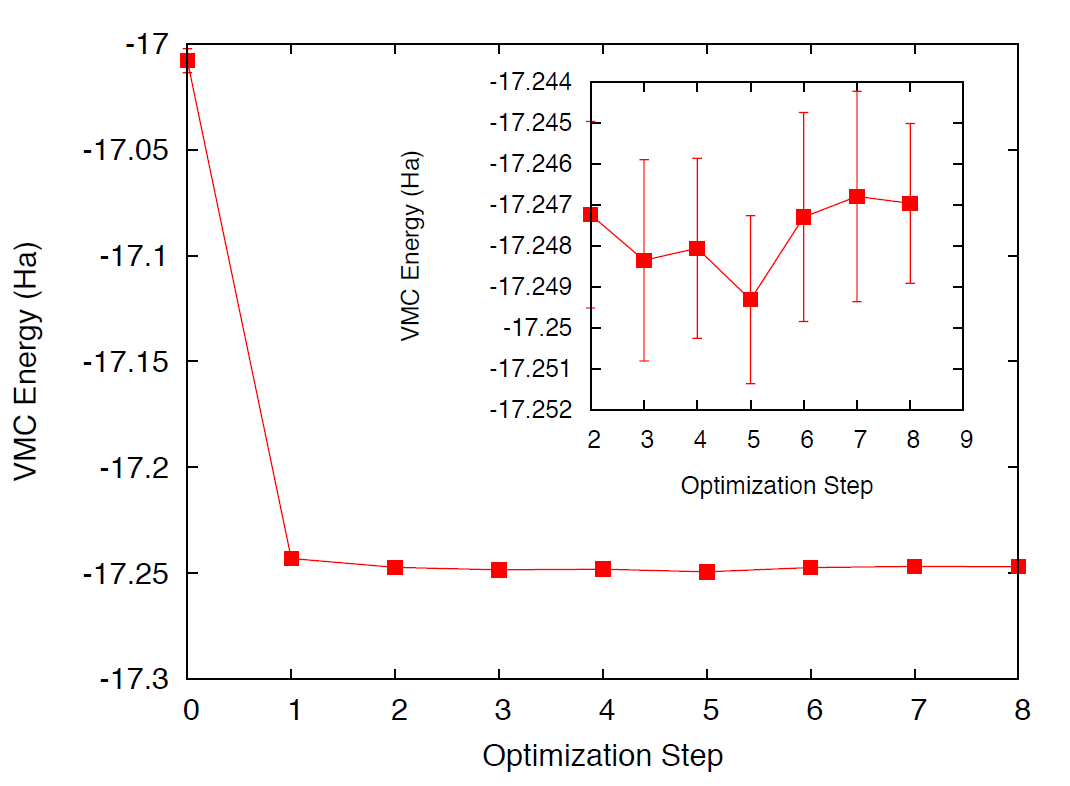
\includegraphics[trim = 0mm 0mm 0mm 0mm, clip,width=0.75\columnwidth]{./figures/lab_advanced_molecules_opt_conv}
\end{center}
\caption{VMC energy as a function of optimization step.
\label{fig:lam_opt_conv}
}
\end{figure}

The resulting energy as a function of optimization step should look qualitatively similar to figure \ref{fig:lam_opt_conv}.
The energy should decrease quickly as a function of the number of optimization steps. After 6-8 steps, the energy should be converged to $\sim$2-3mHa. To improve convergence,
we would need to increase the number of samples used during the optimization. You can
check this for yourself on your free time. With optimized wave-functions we are in a position
to perform VMC and DMC calculations. The modified wave-function files after each step
are written in a file named ID.sNNN.opt.xml, where ID is the identifier of the calculation
defined in the input file (this is defined in the project XML block with parameter “id”) and
NNN is a series number which increases with every executable xml block in the input file.


\subsection{Time-step Study}
Now we will study the dependence of the DMC energy with time-step. From the top directory, 
go to “ex1\_first-run-hartree-fock/dmc\_timestep”. This folder contains a basic xml input
file (dmc\_ts.xml) that performs a short VMC calculation and three DMC calculations
with varying time-steps (0.1, 0.05, 0.01). Link the particle set and the last optimization
file from the previous folder (the file called jopt-h2o.sNNN.opt.xml with the largest value of
NNN). Rename the optimized wave-function to any suitable name if you wish, for example
h2o.opt.xml, and change the name of the particle set and wave-function files in the
input file. An optimized wave-function can be found in the reference files (same location)
in case it is needed. %Using the submission script of the previous exercise as a base, create a
%submission script for this step and submit the run. Set the number of nodes to 32 (2 places
%must be changed), the number of threads to 16 and leave the number of tasks at 1.

The main steps needed to perform this exercise are:
\begin{shaded}
\begin{verbatim}
cd ${TRAINING TOP}/ex1_first-run-hartree-fock/dmc_timestep
cp ../opt/h2o.ptcl.xml ./
cp ../opt/jopt-h2o.s007.opt.xml h2o.opt.wfs.xml
# edit dmc_ts.xml to include the correct ptcl.xml and wfs.xml
jobrun_vesta qmcpack dmc_ts.xml
\end{verbatim}
\end{shaded}
While these runs complete, go to section D and review the basic VMC and DMC input
blocks. Notice that in the current DMC blocks, as the time-step is decreased the number of blocks is also increased. Why is this?

When the simulations are finished, use qmca to analyze the output files and to plot the
DMC energy as a function of time-step. Results should be qualitatively similar to those
presented in figure \ref{fig:lam_dmc_timestep}, in this case we present more time-steps with well converged results to
better illustrate the time-step dependence. In realistic calculations, the time-step must be
chosen small enough so that the resulting error is below the desire accuracy. Alternatively,
various calculations can be performed and the results extrapolated to the zero time-step
limit.


\begin{figure}
\begin{center}
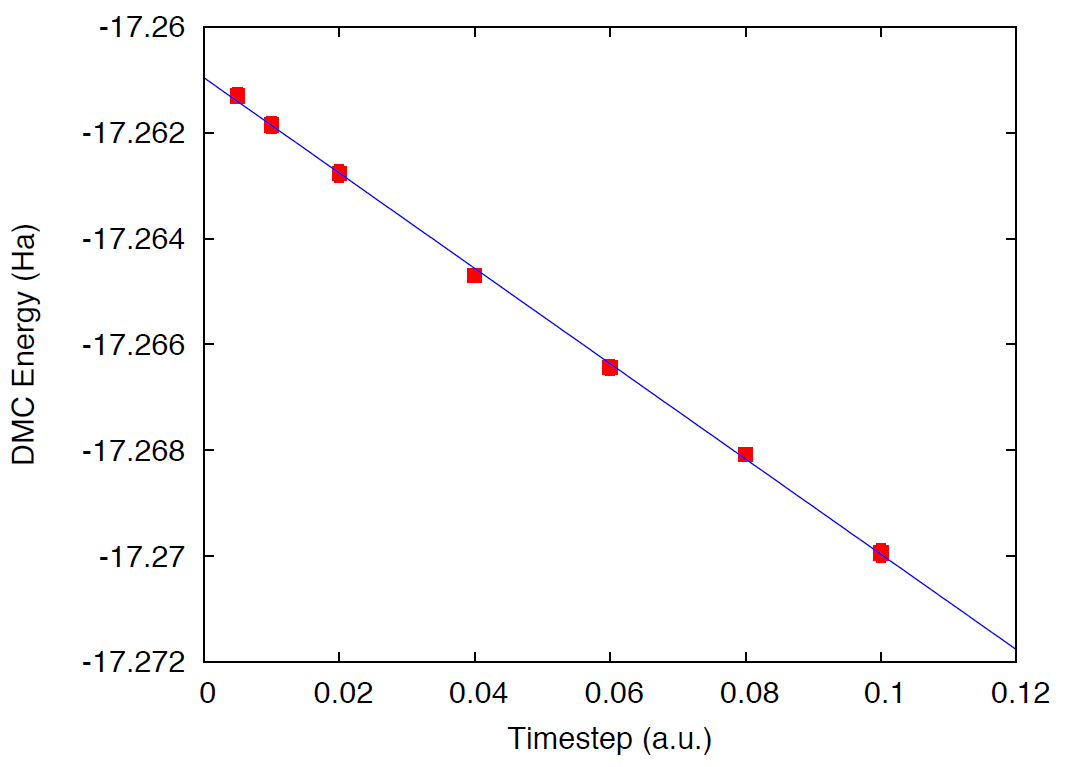
\includegraphics[trim = 0mm 0mm 0mm 0mm, clip,width=0.75\columnwidth]{./figures/lab_advanced_molecules_dmc_timestep}
\end{center}
\caption{DMC energy as a function of timestep.
\label{fig:lam_dmc_timestep}
}
\end{figure}


\subsection{Walker Population Study}
Now we will study the dependence of the DMC energy with the number of walkers in the
simulation. Remember that, in principle, the DMC distribution is reached in the limit of
an infinite number of walkers. In practice, the energy and most properties converge to high
accuracy with $\sim$100-1000 walkers. The actual number of walkers needed in a calculation
will depend on the accuracy of the VMC wave-function and on the complexity and size of
the system. Also notice that using too many walkers is not a problem, at worse it will be
inefficient since it will cost more computer time than necessary. In fact, this is the strategy
used when running QMC calculations on large parallel computers since we can reduce the
statistical error bars efficiently by running with large walker populations distributed across
all processors.

From the top directory, go to ``ex1\_first-run-hartree-fock/dmc\_walkers''. Copy the
optimized wave-function and particle set files used in the previous calculations to the current
folder, these are the ones generated on step 2 of this exercise. An optimized wave-function can be found in the reference files (same location) in case it is needed. The directory
contains a sample DMC input file and submission script. Make 3 directories named NWx,
with x values 120,240,480 and copy the input file to each one. Go
to ``NW120'', and, in the input file, change the name of the wave-function and particle set
files (in this case they will be located one directory above, so use ``../dmc\_timestep/h2.opt.xml'' for
example), change the pseudopotential directory to point to one directory above, change ``targetWalkers'' to 120, change the number of steps to 100, the time-step
to 0.04 and the number of blocks to 400. Notice that ``targetWalkers'' is one way to set the
desired (average) number of walkers in a DMC calculation.   For your own simulations we generally recommend setting $\sim$2*(\#threads)
walkers per node (slightly smaller than this value).

\begin{figure}
\begin{center}
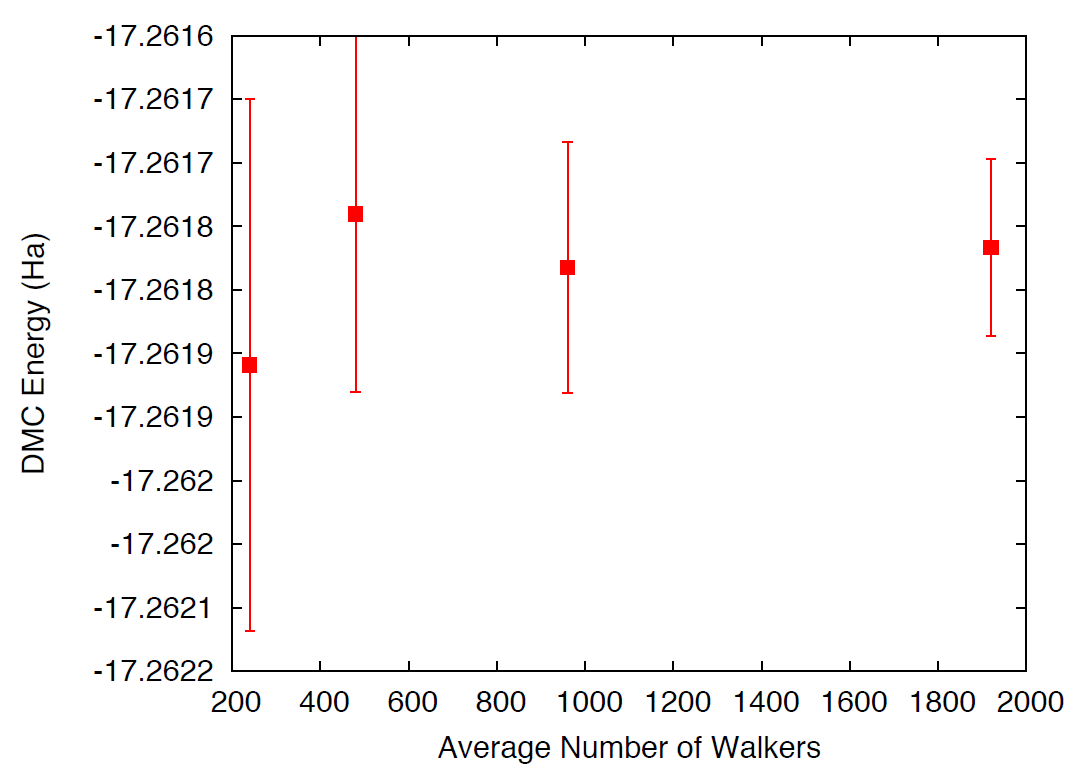
\includegraphics[trim = 0mm 0mm 0mm 0mm, clip,width=0.75\columnwidth]{./figures/lab_advanced_molecules_dmc_popcont}
\end{center}
\caption{DMC energy as a function of the average number of walkers.
\label{fig:lam_dmc_popcont}
}
\end{figure}

Repeat the same procedure in the other folders by setting (targetWalkers=240,
steps=100, timestep=0.04, blocks=200) in NW240 and (targetWalkers=480, 
steps=100, timestep=0.04, blocks=100) in NW480. When
the simulations complete, use qmca to analyze and plot the energy as a function of the
number of walkers in the calculation. As always, figure \ref{fig:lam_dmc_popcont} 
shows representative results of the
dependence of the energy on the number of walkers for a single water molecule. As shown,
less than 240 walkers are needed to obtain an accuracy of 0.1 mHa.


\section{Exercise \#2 Slater-Jastrow Wave-Function Options}
From this point on in the tutorial we assume familiarity with the basic parameters in the
optimization, VMC and DMC XML input blocks of QMCPACK. In addition, we assume
familiarity with the submission system. As a result, the folder structure will not contain
any prepared input or submission files, the student will generate them using generic versions
provided in ``QMCPACK/Generic Files'' and ``GAMESS/Generic Files''. In the case of QMCPACK sample 
files, you will find optm.xml, vmc dmc.xml and submit.csh files. Some of
the options in these files can be left unaltered, but many of them will need to be tailored to
the particular calculation.

In this exercise we will study the dependence of the DMC energy on the choices made
in the wave-function ansatz. In particular, we will study the influence/dependence of the
VMC energy with the various terms in the Jastrow. We will also study the influence of
the VMC and DMC energies on the single particle orbitals used to form the Slater determinant 
in single determinant wave-functions. For this we will use wave-functions generated
with various exchange-correlation functionals in DFT. Finally, we will optimize a simple
multi-determinant wave-function and study the dependence of the energy o the number of
configurations used in the expansion. All of these exercises will be performed on the water 
molecule at equilibrium.


\subsection{Influence of Jastrow on VMC energy with HF wave-function}
In this section we will study the dependence of the VMC energy on the various Jastrow
terms, e.g. one-body, two-body and three-body. From the top directory, go to ``ex2\_slater-jastrow-wf-options/jastrow''. 
We will compare the single determinant VMC energy using a two-body 
Jastrow term, both one- and two-body terms and finally one-, two- and three-body
terms. Since we are interested in the influence of the Jastrow, we will use the HF orbitals
calculated in exercise \#1. Make three folders named 2j,12j,123j. For both 2j and
12j %(we have already optimized a wave-function for the 1-2-3J case, so the steps will be
%slightly different in this case)
, copy the input file optm.xml %and the sample submission file
from ``ex1\_first-run-hartree-fock/opt'' . This input file performs both wave-function optimization 
and a VMC calculation. Copy the un-optimized HF wave-function and particle set files
from ``ex1\_first-run-hartree-fock/convert'', if you followed the instructions in exercise \#1 these should be
named h2o.wfs.xml and h2o.ptcl.xml. Otherwise, you can obtained them from the
REFERENCE files. Modify the file h2o.wfs.xml to remove the appropriate jastrow
blocks. For example, for a two-body Jastrow (only), you need to eliminate the jastrow
blocks named \texttt{<jastrow name="J1"} and \texttt{<jastrow name="J3"}. In the case of 12j, remove
only \texttt{<jastrow name="J3"}. Recommended settings for the optimization run are: nodes=32,
threads=16, blocks=250, samples=128000, time-step=0.5, 8 optimization loops, and in the
VMC section we recommend walkers=16, blocks=1000, steps=1, substeps=100. Notice that
samples should always be set to blocks*threads per node*nodes = 32*16*250=128000. Repeat 
the process in both 2j and 12j cases. For the 123j case, the wave-function has
already been optimized in the previous exercise. Copy the optimized HF wave-function and
the particle set from ``ex1\_first-run-hartree-fock/opt''. Copy the input file from any of the previous runs and remove the optimization block from the
input, just leave the VMC step. In all three cases, modify the submission script and submit the run.

\begin{figure}
\begin{center}
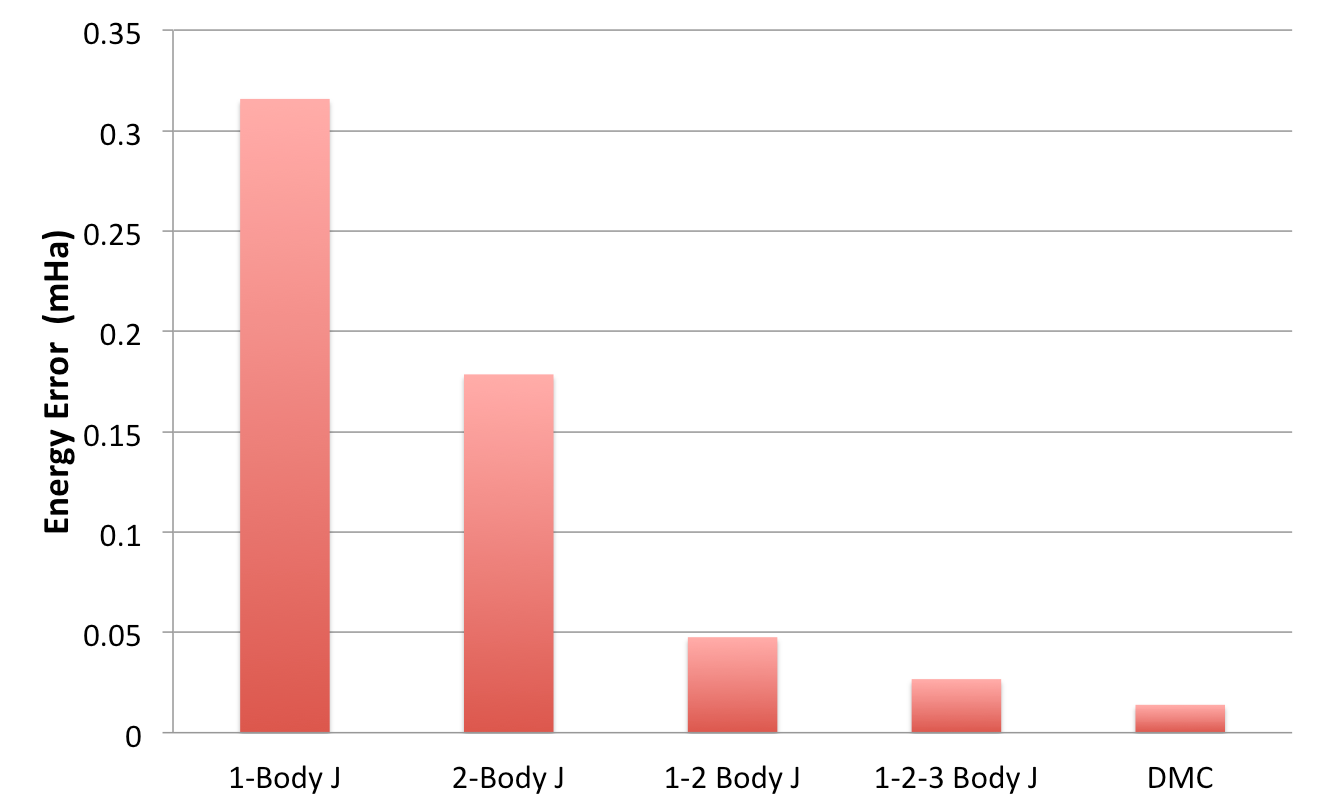
\includegraphics[trim = 0mm 0mm 0mm 0mm, clip,width=0.75\columnwidth]{./figures/lab_advanced_molecules_vmc_jastrow}
\end{center}
\caption{VMC energy as a function of Jastrow type.
\label{fig:lam_vmc_jastrow}
}
\end{figure}

These simulations will take several minutes to complete. This is an excellent opportunity
to go to section E and review the wavefunction XML block used by QMCPACK. When the
simulation are completed, use qmca to analyze the output files. Using your favorite plotting
program (e.g. gnu plot), plot the energy and variance as a function of the Jastrow form.
Figure \ref{fig:lam_vmc_jastrow} shows a typical result for this calculation. As can be seen, the VMC energy and
variance depends strongly on the form of the Jastrow. Since the DMC error bar is directly
related to the variance of the VMC energy, improving the Jastrow will always lead to a
reduction in the DMC effort. In addition, systematic approximations (time-step, number of
walkers, etc) are also reduced with improved wave-functions.


\subsection{Generation of wave-functions from DFT using GAMESS}
In this section we will use GAMESS to generate wave-functions for QMCPACK from
DFT calculations. From the top folder, go to ``ex2\_slater-jastrow-wf-options/orbitals''. In order to demonstrate
the variation in DMC energies with the choice of DFT orbitals, we will choose the following
set of exchange-correlation functionals (PBE, PBE0, BLYP, B3LYP). For each functional,
make a directory using your preferred naming convention (e.g. the name of the functional).
Go into each folder and copy a generic GAMESS input file from %for a ROHF calculation from
``ex1\_first-run-hartree-fock/gms'' .%, a file named rohf.inp should exist.
Rename the file with your preferred naming convention, we suggest using h2o.[dft].inp, where [dft] is the name of
the functional used in the calculation. At this point, this input file should be identical to the
one used to generate the HF wave-function in exercise \#1. In order to perform a DFT
calculation we only need to add ``DFTTYP'' to the \texttt{\$CONTRL ... \$END} section and set
it to the desired functional type, for example ``DFTTYP=PBE'' for a PBE functional. This
variable must be set to (PBE, PBE0, BLYP, B3LYP) to obtain the appropriate functional in
GAMESS. For a complete list of implemented functionals, see the GAMESS input manual.


\subsection{Optimization and DMC calculations with DFT wave-functions}
In this section we will optimize the wave-function generated in the previous step and
perform DMC calculations. From the top directory, go to “ex2\_slater-jastrow-wf-options/orbitals”.
The steps required to achieve this are identical to those used to optimize the wave-function
with HF orbitals. Make individual folders for each calculation and obtain the necessary files
to perform optimization, VMC and DMC calculations from ``ex1\_first-run-hartree-fock/opt'' and ``ex1\_first-run-hartree-fock/dmc\_ts'', for example.
%A file named optm vmc dmc.xml should exist that contains all three execution blocks. 
For each functional, make the appropriate modifications to the input files and copy the particle 
set and wave-function files from the appropriate directory in “ex2\_slater-jastrow-wf-options/orbitals/[dft]”. We
recommend the following settings: nodes=32, threads=16, (in optimization) blocks=250,
samples=128000, timestep=0.5, 8 optimization loops, (in VMC) walkers=16, blocks=100,
steps=1, substeps=100, (in DMC) blocks 400, targetWalkers=960, timestep=0.01. Submit
the runs and analyze the results using qmca .

How do the energies compare against each other? How do they compare against DMC
energies with HF orbitals?
%Orbital Sets and Configurations in 
\section{Exercise \#3: Multi-Determinant Wave-Functions}
In this exercise we will study the dependence of the DMC energy on the set of orbitals
and the type of configurations included in a multi-determinant wave-function. 

\subsection{Generation of a CISD wave-functions using GAMESS}
In this section we will use GAMESS to generate a multi-determinant wave-function with
Configuration Interaction with Single and Double excitations (CISD). In CISD, the Schrodinger equation is solved exactly in a basis of determinants 
including the HF determinant and all its single and double excitations. 

Go to ``ex3\_multi-slater-jastrow/cisd/gms'' and you'll see input and output files named h2o.cisd.inp and h2o.cisd.out. Due to technical problems with GAMESS in the BGQ architecture of VESTA, we are unable to use CISD properly in GAMESS. For this reason, the output of the calculation is  already provided in the directory. 

%You'll see several input and output files named h2o.XXX.inp
%and h2o.XXX.out, where XXX is one of the following multi-determinant methods: CISD,
%CASSCF, CASCI, SOCI. 

There will be time in the next step to study the GAMESS input
files and the description in section A. %In the next exercise we will use the CISD output, in
%the next exercise we will use the remaining files. 
Since the output is already provided, the
only thing needed is to use the converter to generate the appropriate QMCPACK files.  %Copy a submission script from GAMESS/Generic Files and execute the converter for all the output 
%files in the directory (with the exception of CASSCF, which is used to generate orbitals).
%but it doesn’t contain appropriate CI coefficients). 
\begin{shaded}
\begin{verbatim}
jobrun_vesta convert4qmc h2o.cisd.out -ci h2o.cisd.out \
-readInitialGuess 57 -threshold 0.0075
\end{verbatim}
\end{shaded}

We used the PRTMO=.T. flag in the GUESS section, to include orbitals in the output file. You should read these orbitals from the output (-readInitialGuess 40).
The highest occupied orbital in any determinant should be 34, so reading 40 orbitals is a safe choice. In this case, it is important to rename the xml files with meaningful names, for example h2o.cisd.wfs.xml. A threshold of 0.0075 is sufficient for the calculations in the training.


\subsection{Optimization of Multi-Determinant wave-function}

In this section we will optimize the wave-function generated in the previous step. There
is no difference in the optimization steps if a single determinant and a multi-determinant wave-function.
QMCPACK will recognize the presence of a multi-determinant wavefunction and will automatically 
optimize the linear coefficients by default. Go to ``ex3\_multi-slater-jastrow/cisd'' and make a folder called 
thres0.01. Copy the particle set and wavefunction files created in the previous step to the current 
directory. With your favorite text editor, open the wave-function file h2o.wfs.xml. Look for 
the multideterminant XML block and change the ``cutoff'' parameter in detlist to 0.01. Then follow 
the same steps used in the subsection ``Optimization and DMC calculations with DFT wave-functions''
to optimize the wave-function. Similar to this case, design a QMCPACK input file that performs
wave-function optimization followed by VMC and DMC calculations. Submit the calculation.

This is a good time to review the GAMESS input file description in Appendix section A. 
When the run is completed, go to the previous directory and make a new folder named
thres0.0075. Repeat the steps performed above to optimize the wave-function with a cutoff of 0.01, but use a cutoff of 0.0075 this time. This will increase the number of determinants used in the calculation. Notice the ``cutoff'' parameter in the XML should be less than the ``-threshold 0.0075'' flag passed to the converted, which is further bounded by the PRTTOL flag in the GAMESS input.

After the wave-function is generated, we are ready to optimize. Instead of starting from an un-optimized wave-function, we can start from optimized wave-function from thres0.01 to speed up convergence. You will need to modify the file and change the cutoff in detlist to 0.0075 with a text editor. Repeat the optimization steps and submit the calculation.

\begin{figure}
\begin{center}
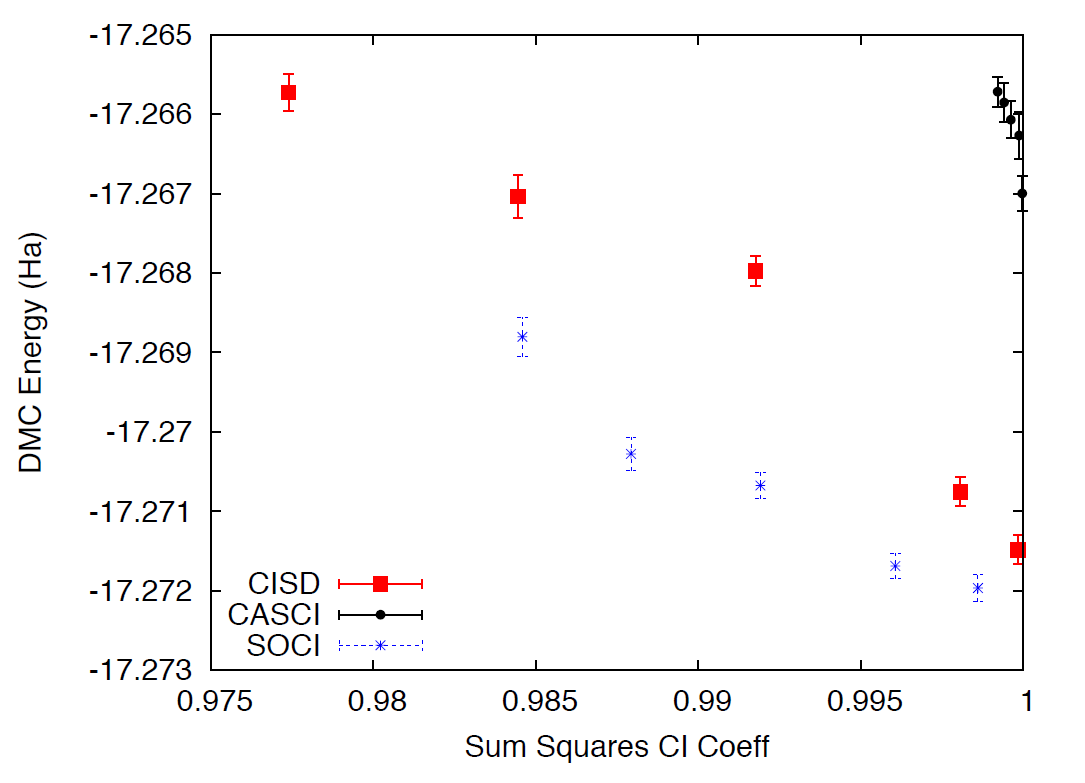
\includegraphics[trim = 0mm 0mm 0mm 0mm, clip,width=0.75\columnwidth]{./figures/lab_advanced_molecules_dmc_ci_cisd}
\end{center}
\caption{DMC energy as a function of the sum of the square of CI coefficients from CISD.
\label{fig:lam_dmc_ci_cisd}
}
\end{figure}

When you are done, use qmca to analyze the results. Compare the energies at these two
coefficient cutoffs with the energies obtained with DFT orbitals. Due to the time limitations of this tutorial it is not practical to optimize the wave-functions with a smaller cutoff, since this would require more samples and longer runs due to the larger number of optimizable parameters. Figure \ref{fig:lam_dmc_ci_cisd} shows the results of such exercise, the DMC energy as a function of the cutoff in the wave-function. As can be seen, a large improvement in the energy is obtained as the number of configurations is increased.


%Since the un-optimized wave-functions were generated in subsection “Generation of a CISD wavefunctions 
%using GAMESS” of exercise \#2, we can skip this section and go straight to the
%wave-function optimization. 

\subsection{CISD, CASCI and SOCI}

Go to “ex3\_multi-slater-jastrow” and inspect folders for the remaining wave-function types: CASCI and SOCI. Follow steps in the previous exercise and obtain the optimized wave-functions for these determinant choices. Notice the SOCI GAMESS output is not included because it is large. Already converted XML inputs can be found in ``ex3\_multi-slater-jastrow/soci/thres*''. %The exercise has already been performed with a CISD wave-function in exercise \#2.

A CASCI wave-function is produced from a CI calculation that includes all the determinants 
in a complete active space (CAS) calculation, in this case using the orbitals from a previous CASSCF
calculation. In this case we used a CAS(8,8) active space, that includes all determinants
generated by distributing 8 electrons in the lowest 8 orbitals. A second-order CI (SOCI) calculation is similar
to the CAS-CI calculation, but in addition to the determinants in the CAS it also includes
all single and double excitations from all of them, leading to a much larger determinant
set. Since we now have considerable experience optimizing wave-functions and calculating
DMC energies, we will leave it to the student to complete the remaining tasks on its own.
If you need help, refer to previous exercises in the tutorial. Perform optimizations for both
wave-functions using cutoffs in the CI expansion of 0.01 an 0.0075. If there is enough time
left, try to optimize the wave-functions with a cutoff of 0.005. Analyze the results and plot
the energy as a function of cutoff for all three cases, CISD, CAS-CI and SOCI.

Figure  \ref{fig:lam_dmc_ci_cisd} shows the result of similar calculations using more samples and smaller cutoffs.
The results should be similar to those produced in the tutorial. For reference, the exact
energy of the water molecule with ECPs is approximately -17.276 Ha. From the results of the
tutorial, how does the selection of determinants is related to the expected DMC energy?
What about the choice in the set of orbitals?


\newpage
\section{Appendix A: GAMESS input}
In this section we provide a brief description of the GAMESS input needed to produce
trial wave-function for QMC calculations with QMCPACK. We assume basic familiarity
with GAMESS input structure, in particular regarding the input of atomic coordinates and
the definition of gaussian basis sets. This section will focus on the generation of the output
files needed by the converter tool, convert4qmc. For a description of the converter, see B.

Only a subset of the methods available in GAMESS can be used to generate wave-functions 
for QMCPACK and we restrict our description here to these.
For a complete description of all the options and methods available
in GAMESS, please refer to the official documentation which could be found in
”http://www.msg.ameslab.gov/gamess/documentation.html”.

Currently, convert4qmc can process output for the following methods in GAMESS (in
SCFTYP) : RHF, ROHF, and MCSCF. Both HF as well as DFT calculations (any DFT
type) could be used in combination with RHF and ROHF calculations. For MCSCF and CI
calculations, ALDET, ORMAS and GUGA drivers can be used (see below for details).


\subsection{HF input}
The following input will perform a restricted HF calculation on a closed-shell singlet 
(multiplicity=1). This will generate RHF orbitals for any molecular system defined in 
\texttt{\$DATA ... \$END}.

\begin{lstlisting}
$CONTRL SCFTYP=RHF RUNTYP=ENERGY MULT=1
ISPHER=1 EXETYP=RUN COORD=UNIQUE MAXIT=200 $END
$SYSTEM MEMORY=150000000 $END
$GUESS GUESS=HUCKEL $END
$SCF DIRSCF=.TRUE. $END
$DATA
...
Atomic Coordinates and basis set
...
$END
\end{lstlisting}

Main options:
\begin{enumerate}
  \item{SCFTYP: Type of SCF method, options: RHF, ROHF, MCSCF, UHF and NONE.}
  \item{RUNTYP: Type of run. For QMCPACK wave-function generation this should always be ENERGY.}
  \item{MULT: Multiplicity of the molecule.}
  \item{ISPHER: Use spherical harmonics (1) or cartesian basis functions (-1).}
  \item{COORD: Input structure for the atomic coordinates in \$DATA.}
\end{enumerate}


\subsection{DFT calculations}
The main difference between the input for a RHF/ROHF calculation and a DFT calculation 
is the definition of the DFTTYP parameter. If this is set in the \$CONTROL
section, a DFT calculation will be performed with the appropriate functional. Notice that
while the default values are usually adequate, DFT calculations have many options involving
the integration grids and accuracy settings. Make sure you study the input manual to be
aware of these. Refer to the input manual for a list of the implemented exchange-correlation
functionals.


\subsection{Multi-Configuration Self-Consistent Field (MCSCF)}
MCSCF calculations are performed by setting SCFTYP=MCSCF in the $CONTROL
section. If this option is set, a $MCSCF section must be added to the input file with the
options for the calculation. An example section for the water molecule used in the tutorial
is shown below.

\begin{lstlisting}
$MCSCF CISTEP=GUGA MAXIT=1000 FULLNR=.TRUE. ACURCY=1.0D-5 $END
\end{lstlisting}

The most important parameter is CISTEP, which defines the CI package used. The only
options compatible with QMCPACK are: ALDET, GUGA, and ORMAS. Depending on the
package used, additional input sections are needed.


\subsection{Configuration Interaction (CI)}
Configuration interaction (full CI, truncated CI, CAS-CI, etc) calculations are performed
by setting SCFTYP=NONE and CITYP=GUGA,ALDET,ORMAS. Each one of this packages 
requires further input sections, which are typically slightly different to the input sections
needed for MCSCF runs.


\subsection{GUGA: Unitary Group CI package}
The GUGA package is the only alternative if one wants CSFs with GAMESS. Below
we provide a very brief description of input sections needed to perform MCSCF, CASCI,
truncated CI and SOCI with this package. For a complete description of these methods and
all the options available, please refer to the GAMESS input manual.

\subsubsection{GUGA-MCSCF}
The following input section performs a CASCI calculation, with a CAS that includes 8
electrons in 8 orbitals (4 DOC and 4 VAL), e.g. CAS(8,8). NMCC is the number of frozen
orbitals (doubly occupied orbitals in all determinants), NDOC is the number of double
occupied orbitals in the reference determinant, NVAL is the number of singly occupied
orbitals in the reference (for spin polarized cases), and NVAL is the number of orbitals in
the active space. Since FORS is set to .TRUE., all configurations in the active space will
be included. ISTSYM defines the symmetry of the desired state.

\begin{lstlisting}
$MCSCF CISTEP=GUGA MAXIT=1000 FULLNR=.TRUE. ACURCY=1.0D-5 $END
$DRT GROUP=C2v NMCC=0 NDOC=4 NALP=0 NVAL=4 ISTSYM=1 MXNINT= 500000 FORS=.TRUE. $END
\end{lstlisting}

\subsubsection{GUGA-CASCI}
The following input section performs a CASCI calculation, with a CAS that includes 8
electrons in 8 orbitals (4 DOC and 4 VAL), e.g. CAS(8,8). NFZC is the number of frozen
orbitals (doubly occupied orbitals in all determinants). All other parameters are identical
to those in the MCSCF input section.

\begin{lstlisting}
$CIDRT GROUP=C2v NFZC=0 NDOC=4 NALP=0 NVAL=4 NPRT=2 ISTSYM=1 FORS=.TRUE. MXNINT= 500000 $END
$GUGDIA PRTTOL=0.001 CVGTOL=1.0E-5 ITERMX=1000 $END
\end{lstlisting}

\subsubsection{GUGA-Truncated CI}
The following input sections will lead to a truncated CI calculation, in this particular case
it will perform a CISD calculation since IEXCIT is set to 2. Other values in IEXCIT will lead
to different CI truncations, for example IEXCIT=4 will lead to CISDTQ. Notice that only
the lowest 30 orbitals will be included in the generation of the excited determinants in this
case. For a full CISD calculation, NVAL should be set to the total number of virtual orbitals.

\begin{lstlisting}
$CIDRT GROUP=C2v NFZC=0 NDOC=4 NALP=0 NVAL=30 NPRT=2 ISTSYM=1 IEXCIT=2 MXNINT= 500000 $END
$GUGDIA PRTTOL=0.001 CVGTOL=1.0E-5 ITERMX=1000 $END
\end{lstlisting}

\subsubsection{GUGA-SOCI}
The following input section performs a SOCI calculation, with a CAS that includes 8
electrons in 8 orbitals (4 DOC and 4 VAL), e.g. CAS(8,8). Since SOCI is set to .TRUE.,
all single and double determinants from all determinants in the CAS(8,8) will be included.

\begin{lstlisting}
$CIDRT GROUP=C2v NFZC=0 NDOC=4 NALP=0 NVAL=4 NPRT=2 ISTSYM=1 SOCI=.TRUE. NEXT=30 MXNINT= 500000 $END
$GUGDIA PRTTOL=0.001 CVGTOL=1.0E-5 ITERMX=1000 $END
\end{lstlisting}


\subsection{ECP}
To use Effective Core Potentials (ECP) in GAMESS, you must define a \{\texttt{\$ECP ... \$END}\} 
block. There must be a definition of a potential for every atom in the system, including
symmetry equivalent ones. In addition, they must appear in the particular order expected
by GAMESS. Below is an example of an ECP input block for a single water molecule using
BFD ECPs. To turn on the use of ECPs, the option “ECP=READ” must be added to the
CONTROL input block.

\begin{lstlisting}
$ECP
O-QMC GEN 2 1
3
6.00000000 1 9.29793903
55.78763416 3 8.86492204
-38.81978498 2 8.62925665
1
38.41914135 2 8.71924452
H-QMC GEN 0 0
3
1.000000000000 1 25.000000000000
25.000000000000 3 10.821821902641
-8.228005709676 2 9.368618758833
H-QMC
$END
\end{lstlisting}


\newpage
\section{Appendix B: convert4qmc}
To generate the particleset and wavefunction XML blocks required by QMCPACK in
calculations with molecular systems, the converter convert4qmc must be used. The converter
will read the standard output from the appropriate Quantum Chemistry calculation and will
generate all the necessary input for QMCPACK. Below we describe the main options of the
converter for GAMESS output. In general, there are 3 ways to use the converter depending
on the type of calculation performed. The minimum syntax for each option is found below.
For a description of the xml files produced by the converter, see section E.

\begin{enumerate}
  \item{For all single determinant calculations (HF and DFT with any DFTTYP):}
  \begin{shaded}
  \begin{verbatim}
    convert4qmc -gamessAscii single det.out
  \end{verbatim}
  \end{shaded}
  \begin{itemize}
    \item{single det.out is the standard output generated by GAMESS.}
  \end{itemize}
  \item{\textit{(This option is not recommended. Use option below to avoid mistakes.)} For 
    multi-determinant calculations where the orbitals and configurations are read from different
    files (for example when using orbitals from a MCSCF run and configurations from a
    subsequent CI run):}
  \begin{shaded}
  \begin{verbatim}
    convert4qmc -gamessAscii orbitals multidet.out -ci cicoeff multidet.out
  \end{verbatim}
  \end{shaded}
  \begin{itemize}
    \item{orbitals\_multidet.out is the standard output from the calculation that generates the
       orbitals. cicoeff multidet.out is the standard output from the calculation that calculates 
       the CI expansion.}
  \end{itemize}
  \item{For multi-determinant calculations where the orbitals and configurations are read from
    the same file, using PRTMO=.T. in the GUESS input block:}
  \begin{shaded}
  \begin{verbatim}
    convert4qmc -gamessAscii multi det.out -ci multi det.out -readInitialGuess Norb
  \end{verbatim}
  \end{shaded}
  \begin{itemize}
    \item{multi\_det.out is the standard output from the calculation that calculates the CI expansion.}
  \end{itemize}
\end{enumerate}

Options:
\begin{itemize}
\item{\textbf{-gamessAscii file.out}: Standard output of GAMESS calculation. With the exception 
of determinant configurations and coefficients in multi-determinant calculations,
everything else is read from this file including: atom coordinates, basis sets, single
particle orbitals, ECPs, number of electrons, multiplicity, etc.}

\item{\textbf{-ci file.out}: In multi-determinant calculations, determinant configurations and 
coefficients are read from this file. Notice that single particle orbitals are NOT read
from this file. Recognized CI packages are: ALDET, GUGA and ORMAS. Output
produced with the GUGA package MUST have the option “NPRT=2” in the CIDRT
or DRT input blocks.}

\item{\textbf{-threshold cutoff}: Cutoff in multi-determinant expansion. Only configurations with
coefficients above this value are printed.}

\item{\textbf{-zeroCI}: Sets to zero the CI coefficients of all determinants, with the exception of the
first one.}

\item{\textbf{-readInitialGuess Norb}: Reads Norb initial orbitals (“INITIAL GUESS ORBITALS”) 
from GAMESS output. These are orbitals generated by the GUESS input
block and printed with the option “PRTMO=.T.”. Notice that this is useful only in
combination with the option “GUESS=MOREAD” and in cases where the orbitals
are not modified in the GAMESS calculation, e.g. CI runs. This is the recommended
option in all CI calculations.}

\item{\textbf{-NaturalOrbitals Norb}: Read Norb “NATURAL ORBITALS” from GAMESS
output. The natural orbitals must exists in the output, otherwise the code aborts.}

\item{\textbf{-add3BodyJ}: Adds three-body Jastrow terms (e-e-I) between electron pairs (both
same spin and opposite spin terms) and all ion species in the system. The radial
function is initialized to zero and the default cutoff is 10.0 bohr. The converter will
add a one- and two-body Jastrow to the wavefunction block by default.}
\end{itemize}

Useful notes:
\begin{itemize}
  \item{The type of single particle orbitals read by the converter depends on the type of
calculation and on the options used. By default, when neither -readInitialGuess or
-NaturalOrbitals are used, the following orbitals are read in each case (notice that
-readInitialGuess or -NaturalOrbitals are mutually exclusive):}
  \begin{itemize}
    \item{RHF and ROHF: “EIGENVECTORS”}
    \item{MCSCF: “MCSCF OPTIMIZED ORBITALS”}
    \item{GUGA, ALDET, ORMAS: Cannot read orbitals without -readInitialGuess or -NaturalOrbitals options.}
  \end{itemize}
  \item{The single particle orbitals and printed CI coefficients in MCSCF calculations are
not consistent in GAMESS. The printed CI coefficients correspond to the next-to-last
iteration, they are not recalculated with the final orbitals. So in order to get appropriate 
CI coefficients from MCSCF calculations, a subsequent CI (no SCF) calculation
is needed to produce consistent orbitals. In principle, it is possible to read the orbitals 
from the MCSCF output and the CI coefficients and configurations from the
output of the following CI calculations. This could lead to problems in principle, since
GAMESS will rotate initial orbitals by default in order to obtain an initial guess consistent 
with the symmetry of the molecule. This last step is done by default and can
change the orbitals reported in the MCSCF calculation before the CI is performed.
In order to avoid this problem, it is highly recommended to use option \#3 above to
read all the information from the output of the CI calculation, this requires the use
of “PRTMO=.T.” in the GUESS input block. Since the orbitals are printed after any
symmetry rotation, the resulting output will always be consistent.}
\end{itemize}


\newpage
\section{Appendix C: Wave-function Optimization XML block}

%\FloatBarrier
\begin{figure}[ht!]
\begin{center}
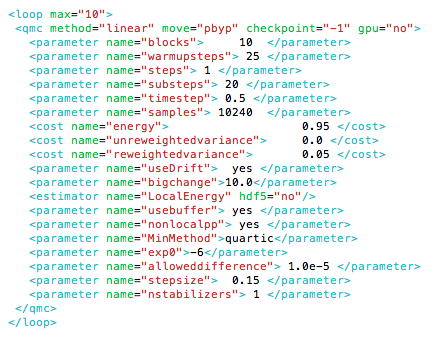
\includegraphics[trim = 0mm 0mm 0mm 0mm, clip,width=0.70\columnwidth]{./figures/lab_advanced_molecules_xml_opt}
\end{center}
\caption{Sample XML optimization block.
\label{fig:lam_xml_opt}
}
\end{figure}
%\FloatBarrier

Options:
\begin{itemize}
  \item{bigchange: (default 50.0) largest parameter change allowed}
  \item{usebuffer: (default no) Save useful information during VMC}
  \item{nonlocalpp: (default no) Include non-local energy on 1-D min}
  \item{MinMethod: (default quartic) Method to calculate magnitude of parameter change
quartic: fit quartic polynomial to 4 values of the cost function obtained using reweighting 
along chosen direction linemin: direct line minimization using reweighting rescale:
no 1-D minimization. Uses Umrigars suggestions.}
  \item{stepsize: (default 0.25) step size in either quartic or linemin methods.}
  \item{alloweddifference: (default 1e-4) Allowed increased in energy}
  \item{exp0: (default -16.0) Initial value for stabilizer (shift to diagonal of H) Actual value
of stabilizer is 10 exp0}
  \item{nstabilizers: (default 3) Number of stabilizers to try}
  \item{stabilizaterScale: (default 2.0) Increase in value of exp0 between iterations.}
  \item{max its: (default 1) number of inner loops with same sample}
  \item{minwalkers: (default 0.3) minimum value allowed for the ratio of effective samples
to actual number of walkers in a reweighting step. The optimization will stop if the
effective number of walkers in any reweighting calculation drops below this value. Last
set of acceptable parameters are kept.}
  \item{maxWeight: (defaul 1e6) Maximum weight allowed in reweighting. Any weight above
this value will be reset to this value.}
\end{itemize}

Recommendations:
\begin{itemize}
  \item{Set samples to equal to (\#threads)*blocks.}
  \item{Set steps to 1. Use substeps to control correlation between samples.}
  \item{For cases where equilibration is slow, increase both substeps and warmupsteps.}
  \item{For hard cases (e.g. simultaneous optimization of long MSD and 3-Body J), set exp0
to 0 and do a single inner iteration (max its=1) per sample of configurations.}
\end{itemize}


\newpage
\section{Appendix D: VMC and DMC XML block}

%\FloatBarrier
\begin{figure}[ht!]
\begin{center}
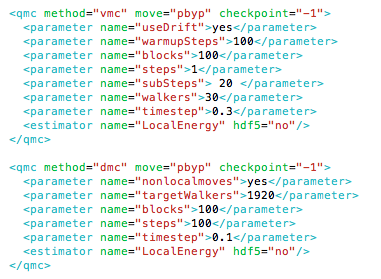
\includegraphics[trim = 0mm 0mm 0mm 0mm, clip,width=0.75\columnwidth]{./figures/lab_advanced_molecules_xml_vmc_dmc}
\end{center}
\caption{Sample XML blocks for VMC and DMC calculations.
\label{fig:lam_xml_vmc_dmc}
}
\end{figure}
%\FloatBarrier

General Options:
\begin{itemize}
\item{\textbf{move}: (default ”walker”) Type of electron move. Options: ”pbyp” and ”walker”.}
\item{\textbf{checkpoint}: (default ”-1”) (If ¿ 0) Generate checkpoint files with given frequency.
The calculations can be restarted/continued with the produced checkpoint files.}
\item{\textbf{useDrift}: (default ”yes”) Defines the sampling mode. useDrift = ”yes” will
use Langevin acceleration to sample the VMC and DMC distributions, while
useDrift=”no” will use random displacements in a box.}
\item{\textbf{warmupSteps}: (default 0) Number of steps warmup steps at the beginning of the
calculation. No output is produced for these steps.}
\item{\textbf{blocks}: (default 1) Number of blocks (outer loop).}
\item{\textbf{steps}: (default 1) Number of steps per blocks (middle loop).}
\item{\textbf{sub steps}: (default 1) Number of substeps per step (inner loop). During sub steps,
the local energy is not evaluated in VMC calculations, which leads to faster execution.
In VMC calculations, set sub steps to the average autocorrelation time of the desired
quantity.}
\item{\textbf{time step}: (default 0.1) Electronic time step in bohr.}
\item{\textbf{samples}: (default 0) Number of walker configurations saved during the current 
calculation.}
\item{\textbf{walkers}: (default \#threads) In VMC, sets the number of walkers per node. The total
number of walkers in the calculation will be equal to walkers*(\# nodes).}
\end{itemize}

Options unique to DMC:
\begin{itemize}
\item{\textbf{targetWalkers}: (default \#walkers from previous calculation, e.g. VMC.) Sets the
target number of walkers. The actual population of walkers will fluctuate around this
value. The walkers will be distributed across all the nodes in the calculation. On a
given node, the walkers are split across all the threads in the system.}
\item{\textbf{nonlocalmoves}: (default ”no”) Set to ”yes” to turns on the use of Casula’s T-moves.}
\end{itemize}


\newpage
\section{Appendix E: Wave-function XML block}

%\FloatBarrier
\begin{figure}[ht!]
\begin{center}
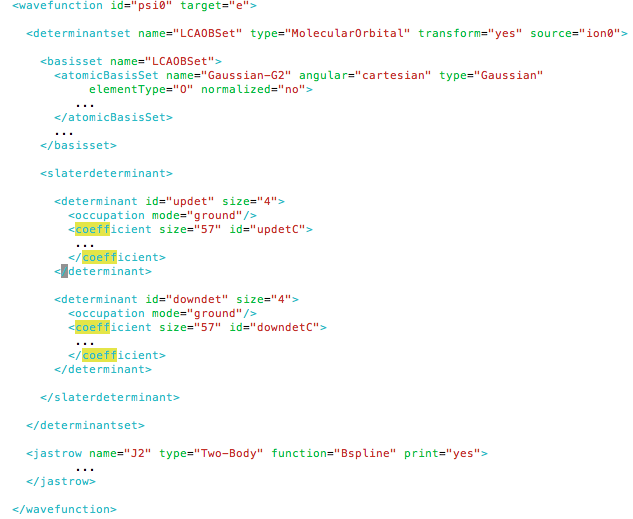
\includegraphics[trim = 0mm 0mm 0mm 0mm, clip,width=1.0\columnwidth]{./figures/lab_advanced_molecules_xml_determinantset}
\end{center}
\caption{Basic framework for a single determinant determinantset XML block.
\label{fig:lam_xml_determinantset}
}
\end{figure}
%\FloatBarrier

In this section we describe the basic format of a QMCPACK wavefunction XML block.
Everything listed in this section is generated by the appropriate converter tools. Little to
no modification is needed when performing standard QMC calculations. As a result, this
section is meant mainly for illustration purposes. Only experts should attempt to modify
these files (with very few exceptions like the cutoff of CI coefficients and the cutoff in Jastrow
functions) since changes can lead to unexpected results.

%\FloatBarrier
\begin{figure}[ht!]
\begin{center}
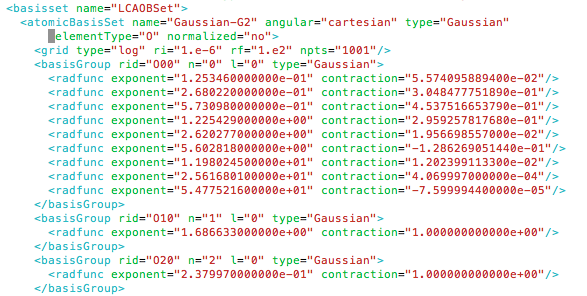
\includegraphics[trim = 0mm 0mm 0mm 0mm, clip,width=1.0\columnwidth]{./figures/lab_advanced_molecules_xml_basisset}
\end{center}
\caption{Sample XML block for an atomic orbital basis set.
\label{fig:lam_xml_basisset}
}
\end{figure}
%\FloatBarrier

A QMCPACK wavefunction XML block is a combination of a determinantset, which
contains the anti-symmetric part of the wave-function, and one or more jastrow blocks.
The syntax of the anti-symmetric block depends on whether the wave-function is a single
determinant or a multi-determinant expansion. Figure \ref{fig:lam_xml_determinantset} 
shows the general structure of the
single determinant case. The determinantset block is composed of a basisset block, which
defines the atomic orbital basis set, and a slaterdeterminant block, which defines the single
particle orbitals and occupation numbers of the Slater determinant. Figure \ref{fig:lam_xml_basisset} 
shows a section
of a basisset block for an oxygen atom. The structure of this block is rigid and should not
be modified. Figure \ref{fig:lam_xml_slaterdeterminant} shows a (piece of a) sample of a 
slaterdeterminant block. The
slaterdeterminant block consists of 2 determinant blocks, one for each electron spin. The
parameter “size” in the determinant block refers to the number of single particle orbitals
present while the “size” parameter in the coefficient block refers to the number of atomic
basis functions per single particle orbital.

%\FloatBarrier
\begin{figure}[ht!]
\begin{center}
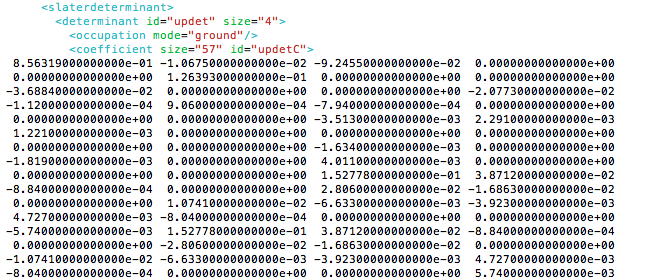
\includegraphics[trim = 0mm 0mm 0mm 0mm, clip,width=1.0\columnwidth]{./figures/lab_advanced_molecules_xml_slaterdeterminant}
\end{center}
\caption{Sample XML block for the single slater determinant case.
\label{fig:lam_xml_slaterdeterminant}
}
\end{figure}
%\FloatBarrier

Figure \ref{fig:lam_xml_multideterminant} shows the general structure of the multi-determinant case. 
Similar to the
single determinant case, the determinantset must contain a basisset block. This definition is
identical to the one described above. In this case, the definition of the single particle orbitals
must be done independently from the definition of the determinant configurations, the latter
is done in the sposet block while the former is done on the multideterminant block. Notice
that 2 sposet sets must be defined, one for each electron spin. The name of reach sposet set
is required in the definition of the multideterminant block. The determinants are defined in
terms of occupation numbers based on these orbitals.

%\FloatBarrier
\begin{figure}[ht!]
\begin{center}
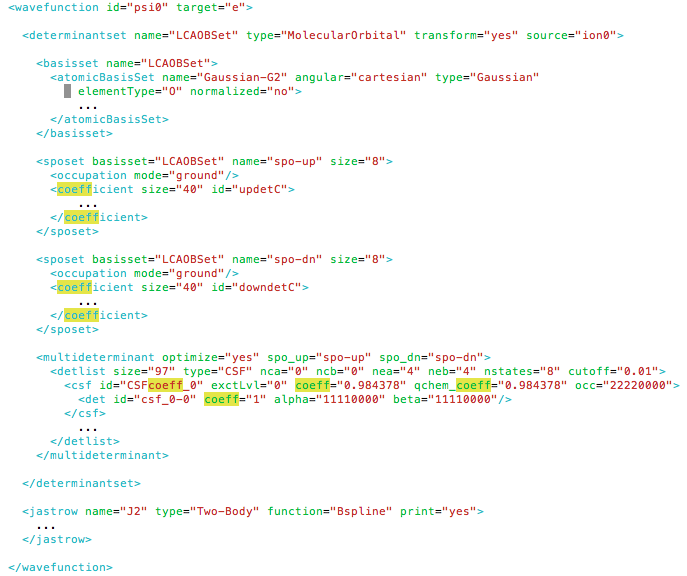
\includegraphics[trim = 0mm 0mm 0mm 0mm, clip,width=1.0\columnwidth]{./figures/lab_advanced_molecules_xml_multideterminant}
\end{center}
\caption{Basic framework for a multi-determinant determinantset XML block.
\label{fig:lam_xml_multideterminant}
}
\end{figure}
%\FloatBarrier

There are various options in the multideterminant block that users should be aware of.
\begin{itemize}
  \item{cutoff: (IMPORTANT! ) Only configurations with (absolute value) “qchem coeff”
larger than this value will be read by QMCPACK.}
  \item{optimize: Turn on/off the optimization of linear CI coefficients.}
  \item{coeff: (in csf ) Current coefficient of given configuration. Gets updated during 
wavefunction optimization.}
  \item{qchem coeff: (in csf ) Original coefficient of given configuration from GAMESS 
calculation. This is used when applying a cutoff to the configurations read from the file.
The cutoff is applied on this parameter and not on the optimized coefficient.}
  \item{nca and nab: number of core orbitals for up/down electrons. A core orbital is an
orbital that is doubly occupied in all determinant configurations, not to be confused
with core electrons. These are not explicitly listed on the definition of configurations.}
  \item{nea and neb: number of up/down active electrons (those being explicitly correlated).}
  \item{nstates: number of correlated orbitals}
  \item{size (in detlist ): contains the number of configurations in the list.}
\end{itemize}
The remaining part of the determinantset block is the definition of jastrow factor. Any
number of these can be defined. Figure \ref{fig:lam_xml_jastrow} shows a sample jastrow 
block including one-, two- and three-body terms. This is the standard block produced by 
convert4qmc with the option -add3BodyJ (this particular example is for a water molecule). 
Optimization of individual radial functions can be turned on/off using the “optimize” 
parameter. It can be added to any coefficients block, even though it is currently not 
present in the J1 and J2 blocks.

%\FloatBarrier
\begin{figure}[ht!]
\begin{center}
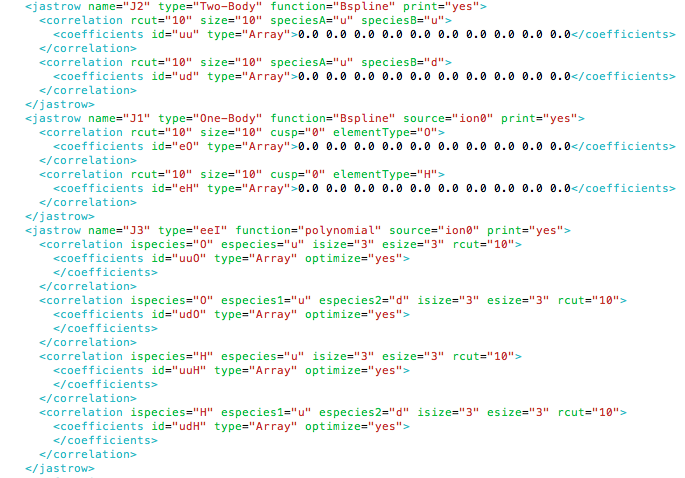
\includegraphics[trim = 0mm 0mm 0mm 0mm, clip,width=1.0\columnwidth]{./figures/lab_advanced_molecules_xml_jastrow}
\end{center}
\caption{Sample Jastrow XML block.
\label{fig:lam_xml_jastrow}
}
\end{figure}
%\FloatBarrier

This training assumes basic familiarity with the UNIX operating system. In particular,
we use simple scripts written in “csh”. In addition, we assume that the student has obtained
all the necessary files and executables, and that the location of the training files are located
at \$\{TRAINING TOP\}.

The goal of the training not only to familiarize the student with the execution and
options in QMCPACK, but also to introduce him/her to important concepts in quantum
Monte Carlo calculations and many-body electronic structure calculations.



\chapter{Lab 4: Using PWSCF and QMCPACK to perform total energy calculations of
condensed systems}

\begin{flushleft}
\textbf{Lab author: Luke Shulenburger}\footnote{Sandia National Laboratories is a multiprogram
laboratory managed and operated by Sandia Corporation, a wholly owned
subsidiary of Lockheed Martin Corporation, for the U.S. Department of Energy's
National Nuclear Security Administration under Contract No.
DE-AC04-94AL85000.}

\textbf{Creation date: July 17, 2014}
\end{flushleft}


The goal of this lab will be to introduce you to the somewhat specialized problems involved in performing diffusion Monte Carlo calculations on condensed matter as opposed to the atoms and molecules that were the focus of earlier labs.   Calculations will be performed on two different systems.  Firstly, we will perform a series of calculations on BCC beryllium focusing on the necessary methodology to limit finite size effects.  Secondly, we will perform calculations on graphene as an example of a system where qmcpack’s ability to handle cases with mixed periodic and open boundary conditions is useful.  This example will also focus on strategies to limit memory usage for such systems.
All of the calculations performed in this lab will utilize the project suite tools that vastly simplify the process by automating the steps of generating trial wavefunctions and performing DMC calculations.

\newcommand{\vp}{\mathbf{a}^\text{p}}
\newcommand{\vs}{\mathbf{a}^\text{s}} 
\newcommand{\Smat}{\mathbf{S}}
\section{Preliminaries}
For any DMC calculation, we must start with a trial wavefunction. As is typical for our calculations of condensed matter, we will produce this wavefunction using density functional theory.  Specifically, we will use quantum espresso to generate a slater determinant of single particle orbitals.  This is done as a three step process.  First, we calculate the converged charge density by performing a DFT calculation with a fine grid of k-points to fully sample the Brilloiun zone.  Next, a non-self consistent calculation is performed at the specific k-points needed for the supercell and twists needed in the DMC calculation (more on this later).  Finally, a wavefunction is converted from the binary representation used by quantum espresso to the portable hdf5 representation used by qmcpack.

The choice of k-points necessary to generate the wavefunctions dependes on both the supercell chosen for the DMC calculation and by the supercell twist vectors needed.  Recall that the wavefunction in a plane wave DFT calculation is written using Bloch's theorem as:
\begin{equation}
\Psi(\vec{r}) = e^{i\vec{k}\cdot\vec{r}}u(\vec{r})
\end{equation}
Where $\vec{k}$ is confined ot the first Brillouin zone of the cell chosen and $u(\vec{r})$ is periodic in this simulation cell.  A plane wave DFT calculation stores the periodic part of the wavefunction as a linear combination of plane waves for each single particle orbital at all k-points selected.  The symmetry of the system allows us to generate an arbitrary supercell of the primitive cell as follows:  Consider the set of primitive lattice vectors, $ \{ \mathbf{a}^p_1, \mathbf{a}^p_2,
\mathbf{a}^p_3\} $.  We may write these vectors in a matrix, $\mathbf{L}_p$, whose
rows are the primitive lattice vectors.  Consider a non-singular
matrix of integers, $\Smat$.  A corresponding set of supercell lattice
vectors, $\{\mathbf{a}^s_1, \mathbf{a}^s_2, \mathbf{a}^s_3\}$, can be constructed by the matrix
product 
\begin{equation}
\mathbf{a}^s_i = S_{ij} \mathbf{a}^p_j
\end{equation}
If the primitive cell contains $N_p$ atoms, the supercell will then
contain $N_s = |\det(\Smat)| N_p$ atoms.

Now, the wavefunciton at any point in this new supercell can be related to the wavefunction in the primitive cell by  finding the linear combination of primitive lattice vectors that maps this point back to the primitive cell:
\begin{equation}
\vec{r}' = \vec{r} + x \mathbf{a}^p_1 + y \mathbf{a}^p_2 + z\mathbf{a}^p_3 = \vec{r} + \vec{T}
\end{equation}
where $x, y, z$ are integers.   Now the wavefunction in the supercell at point $\vec{r}'$ can be written in terms of the wavefunction in the primitive cell at $\vec{r}'$ as:
\begin{equation}
\Psi(\vec{r}) = \Psi(\vec{r}') e^{i \vec{T} \cdot \vec{k}}
\end{equation}
where $\vec{k}$ is confined to the first Brillouin zone of the primitive cell.  We have also chosen the supercell twist vector which places a constraint on the form of the wavefunction in the supercell.  The combination of these two constraints allows us to identify family of N k-points in the primitive cell that satisfy the constraints.  Thus for a given supercell tiling matrix and twist angle, we can write the wavefunction everywhere in the supercell by knowing the wavefunction a N k-points in the primitive cell.  This means that the memory necesary to store the wavefunction in a supercell is only linear in the size of the supercell rather than the quadratic cost if symmetry were neglected.

\section{Total energy of BCC beryllium}

As was discussed in this morning’s lectures when performing calculations of periodic solids with QMC, it is essential to work with a reasonable size supercell rather than the primitive cells that are common in mean field calculations.  Specifically, all of the finite size correction schemes discussed in the morning require that the exchange-correlation hole be considerably smaller than the periodic simulation cell.  Additionally, finite size effects are lessened as the distance between the electrons in the cell and their periodic images increases, so it is advantageous to generate supercells that are as spherical as possible so as to maximize this distance.  However, there is a competing consideration in that for calculating total energies we often want to be able to extrapolate the energy per particle to the thermodynamic limit by means of the following formula in 3 dimensions:
\begin{equation}
E_{\inf} = C + E_{N}/N
\end{equation}
This formula derived assuming the shape of the supercells is consistent (more specifically that the periodic distances scale uniformly with system size), meaning we will need to do a uniform tiling, ie, 2x2x2, 3x3x3 etc.  As a 3x3x3 tiling is 27 times larger than the supercell and the practical limit of DMC is on the order of 200 atoms (depending on Z), sometimes it is advantagous to choose a less spherical supercell with fewer atoms rather than a more spherical one that is too expensive to tile.

In the case of a BCC crystal, it is possible to tile the one atom primitive cell to a cubic supercell by only doubling the number of electrons.  This is the best possible combination of a small number of atoms that can be tiled and a regular box that maximizes the distance between periodic images.  We will need to determine the tiling matrix S that generates this cubic supercell by solving the following equation for the coefficients of the S matrix:
\begin{equation}
 \left[\begin{array}{rrr}
  1 & 0 & 0 \\
  0 & 1 & 0 \\
  0 & 0 & 1 
  \end{array}\right] =  \left[\begin{array}{rrr}
  s_{11} & s_{12} & s_{13} \\
  s_{21} & s_{22} & s_{23} \\
  s_{31} & s_{32} & s_{33} 
  \end{array}\right] \cdot 
\left[\begin{array}{rrr}
  0.5 &  0.5 & -0.5 \\
 -0.5 &  0.5 &  0.5 \\
  0.5 & -0.5 &  0.5
\end{array}\right] 
\end{equation}

We will now use the project suite to generate the trial wavefunction for this BCC beryllium.

Fortunately, the project-suite will handle determination of the proper k-vectors given the tiling matrix.  All that is needed is to place the tiling matrix in the Be-2at-setup.py file.   Now the definition of the physical system is:

\begin{lstlisting}
    bcc_Be = generate_physical_system(
        lattice    = 'cubic',
        cell       = 'primitive',
        centering  = 'I',
        atoms      = 'Be',
        constants  = 3.490,
        units      = 'A',
        net_charge = 0,
        net_spin   = 0,
        Be         = 2,
        tiling     = [[a,b,c],[d,e,f],[g,h,i]],
        kgrid      = kgrid,
        kshift     = (.5,.5,.5)
        )
\end{lstlisting}
Where the tiling line should be replaced with the row major tiling matrix from above.  This script file will now perform a converged DFT calculation to generate the charge density in a directory called bcc-beryllium/scf and perform a non self consistend DFT calculation to generate single particle orbitals in the direcotry bcc-beryllium/nscf.  Fortunately, the project suite will calculate the required k-points needed to tile the wavefunction to the supercell, so all that is necessary is the granularity of the supercell twists and whether this grid is shifted from the origin.  Once this is finished, it performs the conversion from pwscf's binary format to the hdf5 format used by qmcpack.  Finally, it will optimize the coefficients of one-body and two-body jastrow factors in the supercell defined by the tiling matrix.

Run these calculations by executing the script Be-2at-setup.py.  You will notice that such small calcuations as are required to generate the wavefunction of Be in a one atom cell are rather inefficent to run on a high performance computer such as vesta in terms of the time spent doing calculations versus time waiting on the scheduler and booting compute nodes.  One of the benefits of the portable hdf format that is used by qmcpack is that you can generate data like wavefunctions on a local workstation or other convenient resource and only use high performance clusters for the more expensive QMC calculations.

In this case, the wavefunction is generated in the directory bcc-beryllium/nscf-2at\_222/pwscf\_output in a file called pwscf.pwscf.h5.  It can be useful for debugging purposes to be able to verify the contents of this file are what you expect.  For instance, you can use the tool h5ls to check the geometry of the cell where the dft calculations were performed, or number of k-points or electrons in the calculation.  This is done with the command: h5ls -d pwscf.pwscf.h5/supercell or h5ls -d pwscf.pwscf.h5/electrons.

In the course of running Be-2at-setup.py, you will get an error when attempting to perform the vmc and wavefunction optimization calculations.  This is due to the fact that the wavefunction has been generated supercell twists of the form (+/- 1/4, +/- 1/4, +/- 1/4).  In the case that the supercell twist contains only 0 or 1/2, it is possible to operate entirely with real arithmetic.  The executabe that has been indicated in Be-2at-setup.py has been compiled for this case.  Note that where this is possible, the memory usage is a factor of two less than the general case and the calculations are somewhat faster.  However, it is often necessary to perform calculations away from these special twist angles in order to reduce finite size effects.  To fix this, delete the directory bcc-beryllium/opt-2at, change the line in near the top of Be-2at-setup.py from 
\begin{lstlisting}
qmcpack    = '/soft/applications/qmcpack/build_XL_real/bin/qmcapp'
\end{lstlisting}
to
\begin{lstlisting}
qmcpack    = '/soft/applications/qmcpack/build_XL_complex/bin/qmcapp'
\end{lstlisting}
and rerun the script.

When the optimiztion calculation has finished, check that everything as proceeded correctly by looking at the output in the opt-2at directory.  Firstly, you can grep the output file for Delta to see if the cost function has indeed been decreasing during the optimization.  You should find something like:
\begin{lstlisting}
 OldCost: 4.8789147e-02 NewCost: 4.0695360e-02 Delta Cost:-8.0937871e-03
 OldCost: 3.8507795e-02 NewCost: 3.8338486e-02 Delta Cost:-1.6930674e-04
 OldCost: 4.1079105e-02 NewCost: 4.0898345e-02 Delta Cost:-1.8076319e-04
 OldCost: 4.2681333e-02 NewCost: 4.2356598e-02 Delta Cost:-3.2473514e-04
 OldCost: 3.9168577e-02 NewCost: 3.8552883e-02 Delta Cost:-6.1569350e-04
 OldCost: 4.2176276e-02 NewCost: 4.2083371e-02 Delta Cost:-9.2903058e-05
 OldCost: 4.3977361e-02 NewCost: 4.2865751e-02 Delta Cost:-1.11161830-03
 OldCost: 4.1420944e-02 NewCost: 4.0779569e-02 Delta Cost:-6.4137501e-04
\end{lstlisting}
Which shows that the starting wavefunction was fairly good and that most of the optimizaiton occurred in the first step.  Confirm this by using qmca to look at how the energy and variance changed over the course of the calculation with teh comand: qmca -q ev -e 10 *.scalar.dat executed in the opt-2at directory.  You should get output like the following:
\begin{lstlisting}
                 LocalEnergy               Variance             ratio
opt  series 0  -2.159139 +/- 0.001897   0.047343 +/- 0.000758   0.0219 
opt  series 1  -2.163752 +/- 0.001305   0.039389 +/- 0.000666   0.0182 
opt  series 2  -2.160913 +/- 0.001347   0.040879 +/- 0.000682   0.0189 
opt  series 3  -2.162043 +/- 0.001223   0.041183 +/- 0.001250   0.0190 
opt  series 4  -2.162441 +/- 0.000865   0.039597 +/- 0.000342   0.0183 
opt  series 5  -2.161287 +/- 0.000732   0.039954 +/- 0.000498   0.0185 
opt  series 6  -2.163458 +/- 0.000973   0.044431 +/- 0.003583   0.0205 
opt  series 7  -2.163495 +/- 0.001027   0.040783 +/- 0.000413   0.0189 
\end{lstlisting}

Now that the optimization has completed successfully, we can perform dmc calculations.  The first goal of the calculations will be to try to eliminate the one body finite size effects by twist averaging.  The script Be-2at-qmc.py has the necessary input.  Note on line 42 two twist grids are specified, (2,2,2) and (3,3,3).  Change the tiling matrix in this input file as in Be-2at-qmc.py and start the calculations.  Note that this workflow takes advantage of qmcpack's ability to group jobs.  If you look in the directory dmc-2at\_222 at the job submission script, (dmc.qsub.in) you will note that rather than operating on an xml input file, qmcapp is targeting a text file called dmc.in.  This file is a simple text file that contains the names of the 8 xml input files needed for this job, one for each twist.  When operated in this mode, qmcpack will use mpi groups to run multiple copies of itself within the same mpi context.  This is often useful both in terms of organizing calculations and also for taking advantage of the large job sizes that computer centers often encourage.

The dmc calculations in this case are designed to complete in a few minutes.  When they have finished running, first look at the scalar.dat files corresponding to the dmc calculations at the various twists in dmc-2at\_222.  Using a command like 'qmca -q ev -e 32 *.s001.scalar.dat' (with a suitably chosen number of blocks for the equilibration), you will see that the dmc energy in each calcuation is nearly identical within the statistical uncertainty of the calculations.  In the case of a large supercell, this is often indicative of a situation where the Brilloiun zone is so small that the one body finite size effects are nearly converged without any twist averaging.  In this case, however, this is because of the symmetry of the system.  For this cubic supercell, all of the twist angles chosen in this shifted 2x2x2 grid are equivalent by symmetry.  In the case where substantial resources are required to equilibrate the dmc calculations, it can be beneficial to avoid repeating such twists and instead simply weight them properly.  In this case however where the equilibration is inexpensive, there is no benefit to adding such complexity as the calculations can simply be averaged together and the result is equivalent to performing a single longer calcuation.

Using the command qmc -a -q ev -e 16 *.s001.scalar.dat, average the dmc energies in dmc-2at\_222 and dmc-2at\_333 to see whether the one body finite size effects are converged with a 3x3x3 grid of twists.  As beryllium as a metal, the convergence is quite poor (~0.025 Ha / Be or ~ 0.7 eV / Be).  If this were a production calculation it would be necessary to perform calculations on much larger grids of supercell twists to eliminate the one body finite size effects.

In this case there are several other calculations that would warrent a high priority.  A script Be-16at-qmc.py has been provided where you can imput the appropriate tiling matrix for a 16 atom cell and perform calculations to estimate the two body finite size effects which will also be quite large in the 2 atom calculations.  This script will take approximately 30 minutes to run to completion, so depending on interest,  you can either run it, or also work to modify the scripts to address the other technical issues that would be necessary for a production calculation such as calculating the population bias or the timestep error in the dmc calculations.  

Another useful exercise would be to attempt to validate this pseudopotential by calculating the ionization potential and electron affinity of the isolated atom and comparing to the experimental values:  IP = 9.3227 eV , EA = 2.4 eV.

\section{Handling a 2D system: graphene}
In this section we will examine a calculation of an isolated sheet of graphene.  As graphene is a two dimensional system, we will take advantage of qmcpack's ability to mix periodic and open boundary conditions to eliminate and spurious interaction of the sheet with its images in the z direction.  Run the script graphene-setup.py which will generate the wavefunction and optimize one and two body jastrow factors.  In the script, notice line 160: bconds = 'ppn' in the generate\_qmcpack function which specifies this mix of open and periodic boundary conditions.  As a consequence of this, the atoms will need to be kept away from this open boundary in the z direction as the electronic wavefunction will not be defined outside of the simulation box in this direction.  For this reason, all of the atom positions in at the beginning of the file have z coordinates 7.5.  At this point, run the script graphene-setup.py.

Aside from the change in boundary conditions, the main thing that distinguished this kind of calculation from the beryllium example above is the large amount of vacuum in the cell.  While this is a very small calculation designed to run quickly in the tutorial, in general a more converged calculation would quickly become memory limited on an architecture like BG/Q.  When the initial wavefunciton optimizaiton has completed to your satisfaction, run the scripts graphene-loop-buffer.py and graphene-loop-mesh.py.  These examine within variational Monte Carlo two approaches to reducing the memory required to store the wavefunction.  In graphene-loop-mesh.py, the spacing between the b-spline points is varied uniformly.  The mesh spacing is a prefactor to the linear spacing between the spline points, so the memory usage goes as the cube of the meshfactor.  When you run the calculations, examine the .s000.scalar.dat files with qmca to determine the lowest possible mesh spacing that preserves both the vmc energy and the variance.  Similarly, the script graphene-loop-buffer.py uses a feature which generates two spline tables for the wavefunction.  One will have half of the mesh spacing requested in the input file and will be valid everywhere.  The second one will only be defined in the smallest parallelpiped that contains all of the atoms in the simulation cell with minimum distance given by the buffer size.  Again, see what the smallest possible buffer size is that preserves the vmc energy and variance.

Finally, edit the file graphene-final.py which will perform two DMC calculations.  In the first, (qmc1) replace the following lines:
\begin{lstlisting}
    meshfactor   = xxx,
    precision    = '---',
    truncate     = False,
    buffer       = 0.0,
\end{lstlisting}
using the values you have determined to perform the calculation with as small as possible of wavefunction.  Note that we can also use single precision arithmetic to store the wavefunction by specifying precision='single'.  When you run the script, compare the output of the two DMC calculations in terms of energy and variance.  Also see if you can calculate the fraction of memory that you were able to save by using a meshfactor other than 1, a buffer table and single precision arithmetic.

\section{Conclusion}
Upon completion of this lab, you should be able to use the project suite to perform DMC calculations on periodic solids when provided with a pseudopotential.  You should also be able to reduce the size of the wavefunction in a solid state calculation in cases where memory is a limiting factor.

\section{Acknowledgment}
 This tutorial was created with support from Sandia National Laboratories.

 Sandia National Laboratories is a multiprogram laboratory managed and operated by
 Sandia Corporation, a wholly owned subsidiary of Lockheed Martin Corporation, for
 the U.S. Department of Energy's National Nuclear Security Administration under
 Contract No. DE-AC04-94AL85000.

\chapter{Lab 5: Excited State Calculations}
\label{chap:excited}

\hide{
	\begin{flushleft}
		\textbf{Lab author: Kayahan Saritas}\footnote{Oak Ridge National Laboratory}
		
		\textbf{Creation date: November 29, 2018}
	\end{flushleft}
}

\section{Topics covered in this Lab}
\begin{itemize}
	\item{Tiling DFT primitive cells into optimal QMC supercells}
	\item{Fundamentals of  between neutral and charged calculations}
	\item{Calculating quasiparticle excitation energies of condensed matter systems}
	\item{Calculating optical excitation energies of condensed matter systems}
\end{itemize}

\section{Lab directories and files}

\begin{shade}
labs/lab5_excited_properties/
    band.py           - Band structure calculation for Carbon Diamond
    optical.py        - VMC optical gap calculation using the tiling matrix from band.py
    quasiparticle.py  - VMC quasiparticle gap calculation using the tiling matrix from band.py
pseudopotentials      - pseudopotential directory
	C.BFD.upf         - C PP for Quantum ESPRESSO
	C.BFD.xml         - C PP for QMCPACK
\end{shade}

The goal of this lab is to perform neutral and charged excitation calculations in condensed matter systems using QMCPACK. 
Throughout this lab, a working knowledge of \textit{Lab4 Condensed Matter Calculations} is assumed. 
First, we will introduce the concepts of neutral and charged excitations. 
We will briefly discuss these in relation to the specific experimental studies that must be used to benchmark DMC results. 
Secondly, we will perform charged (quasiparticle) and neutral (optical) excitations calculations on C-diamond.

\section{Basics and excited state experiments}
Although VMC and DMC methods are better suited for studying ground state properties of materials, they can still provide useful information regarding the excited states. 
Unlike the applications of band structure theory such as DFT and GW, it is more challenging to obtain the complete excitation spectra using DMC. 
However, it is relatively straightforward to calculate the band gap minimum of a condensed matter system using DMC. 

We will briefly discuss the two main ways of obtaining the band gap minimum through experiments: photoemission and absorption studies.  
The energy required to remove an electron from a neutral system is called the ionization potential (IP), which is available from direct photoemission experiments. 
In contrast, the emission energy of a negatively charged system (or the energy required to convert a negatively charged system to a neutral system) known as electron affinity (EA) and it is available from inverse photoemission experiments. 
Outline of these experiments are shown in Fig. \ref{fig:lab_ex_exp}. 

Following the explanation in the previous paragraph and Fig. \ref{fig:lab_ex_exp}, the \textit{quasiparticle} band gap of a material can be defined as:
\begin{equation}
	E_g=EA-IP=(E_{N+1}^{CBM}-E_{N}^{K'})-(E_{N}^{K'}-E_{N-1}^{VBM})=E_{N+1}^{CBM}+E_{N-1}^{VBM}-2*E_{N}^{K'}\label{eq:qp}
\end{equation}
where $N$ is the number of electrons in the neutral system and $E_{N}$ is the ground state energy of the neutral system. 
CBM and VBM stand for the conduction band minimum and valence band maximum, respectively. K' can formally be arbitrary at the infinite limit.
However, in practical calculations, a supertwist which accommodates both CBM and VBM can be more efficient in terms of computational time and systematic finite size error cancellation. 
In the literature, the quasiparticle gap is also called the electronic gap. 
The term electronic comes from the fact that in both photoemission experiments, it is assumed that the perturbed electron is non-interacting with the sample. 

\begin{figure}
	\centering
	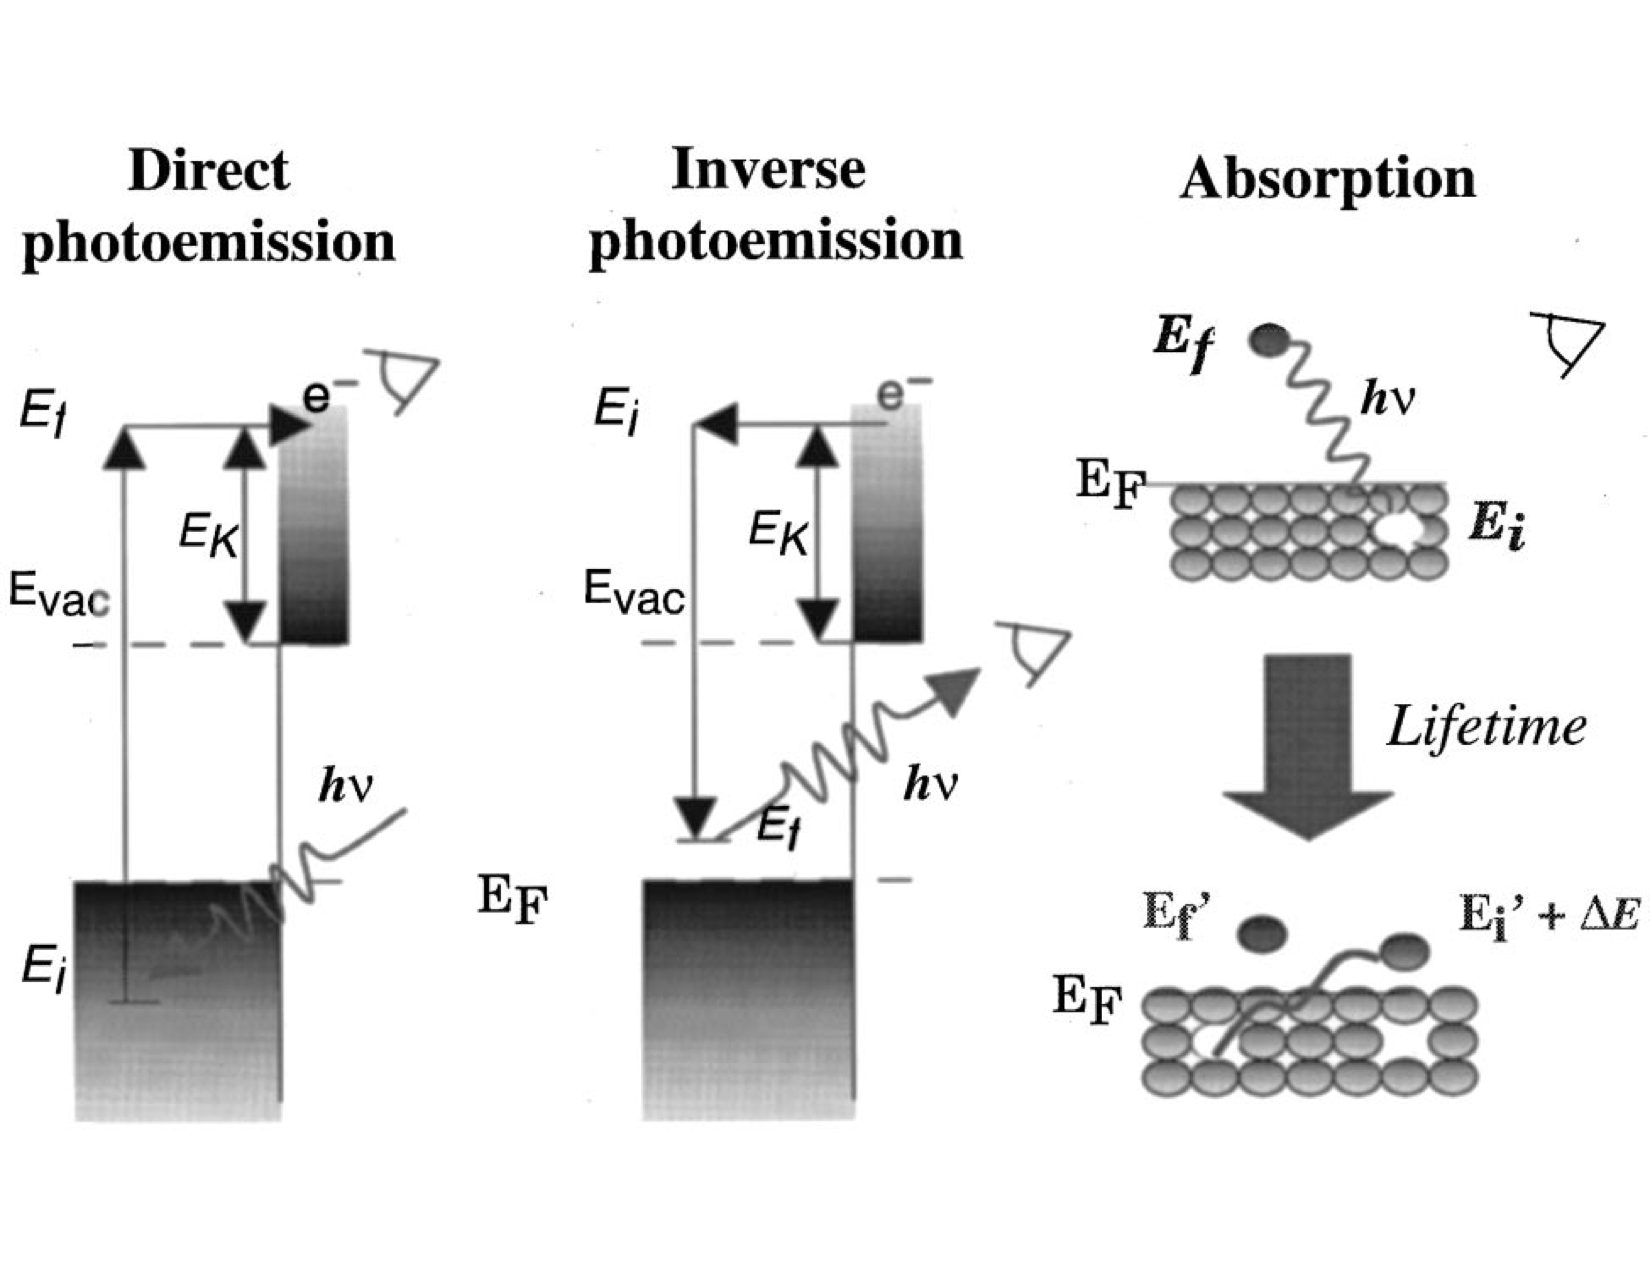
\includegraphics[width=0.5\textwidth]{./figures/lab_excited_experiments}
	\caption{Direct and inverse photoemission experiments involve charged excitations, whereas optical absorption experiments involves excitation that are just enough to be excited to the conduction band. From ref. \cite{Onida2002a}}
	\label{fig:lab_ex_exp}
\end{figure}

Additionally, one can also perform absorption experiments where electrons are perturbed at relatively lower energies, just enough to be excited into the conduction band. 
In absorption experiments,  electrons are perturbed at lower energies. 
Therefore, they are not completely free and the system is still considered neutral. 
Since a \textit{quasihole} and \textit{quasielectron} are formed simultaneously, it creates a bound state, unlike the free electron in the quasiparticle gap as described above. 
This process is also known as \textit{optical} excitation, which is schematically shown in Fig. \ref{fig:lab_ex_exp}, under "Absorption". 
The optical gap can be formulated as follows:
\begin{equation}
E_g^{K_1 {\rightarrow} K_2}=E^{K_1 {\rightarrow} K_2}- E_{0}\label{eq:optical}
\end{equation}
where $E^{K_1 {\rightarrow} K_2}$ is the energy of the system when a valence electron at wavevector $K_1$ is promoted to the conduction band at wavevector $K_2$. 
Therefore, the $E_g^{K_1 {\rightarrow} K_2}$ is called the optical gap for promoting an electron at $K_1$ to $K_2$.
If both CBM and VBM are on the same k-vector then the material is called direct band gap, since it can directly emit photons without any external perturbation (phonons). 
However, if CBM and VBM share different k-vectors, then the photon emitting electron has to transfer some of its momenta to the crystal lattice and then decay to the ground state. 
As this process involves an intermediate step, this property is called the indirect band gap. 
Difference between the optical and electronic band gaps are called the exciton binding energy. 
Exciton binding energy is very important for optoelectronic applications such as lasers. 
Since the recombination usually occurs between free holes and free electrons, a bound electron and hole state means that the spectrum of emission energies will be narrower. 
In the examples that follow, we will investigate the optical excitations of C-diamond.

\begin{figure}
	\hfill
	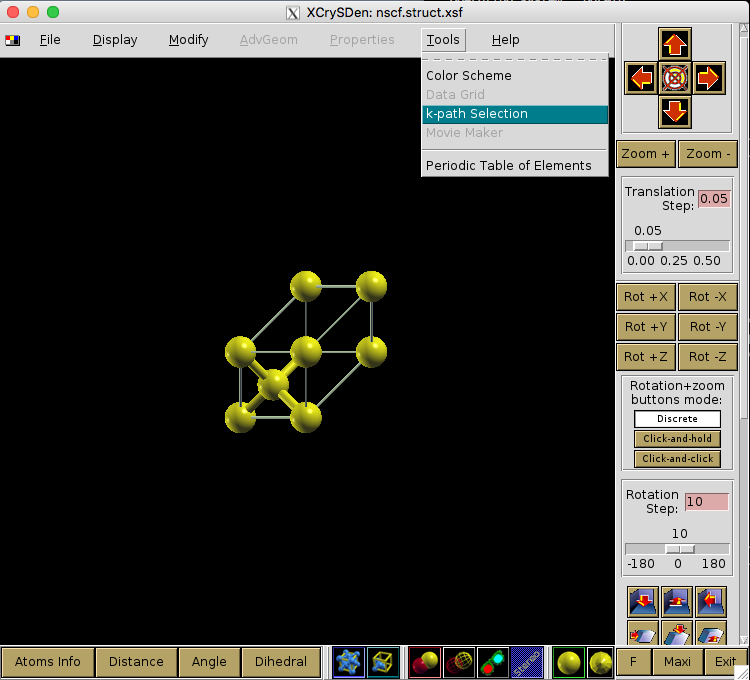
\includegraphics[width=0.41\textwidth]{./figures/lab_excited_xcrysden1}
	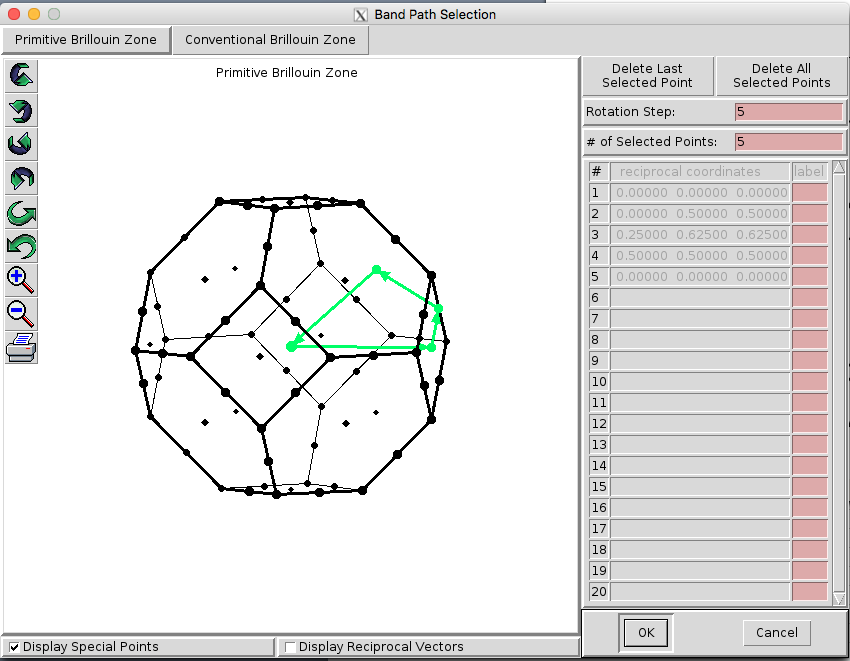
\includegraphics[width=0.48\textwidth]{./figures/lab_excited_xcrysden2}
	\hfill
	\caption{Visualizing the Brillouin Zone using XCRYSDEN.}
	\label{fig:lab_ex_xcrysden}
\end{figure}


\section{Preparation for the excited state calculations}\label{sec:lab_ex_prep}

In this section, we will study the preparation steps to perform excited state calculations with quantum Monte Carlo. 
Here, the most basic steps are listed in the implementation order:
\begin{enumerate}
	\item Identify the high symmetry k-points of the standardized primitive cell 
	\item Perform DFT band structure calculation along high symmetry paths
	\item Find a supertwist which includes all the k-points of interest
	\item Identify the indexing of k-points in the supertwist to be used in QMCPACK
\end{enumerate}

\subsection{Identifying high-symmetry k-points}\label{sec:lab_ex_highk}
Primitive cell is the most basic, non-unique repeat unit of a crystal in the real space. 
However, the translations of the repeat unit, the Bravais lattice is unique for each crystal, and can be represented using discrete translation operations, $R_n$:
\begin{equation}
{\bf R_n} = n_1{\bf a_1} + n_2{\bf a_2} + n_3{\bf a_3}
\end{equation}
$a_n$ are the real space lattice vectors in three dimensions. Thanks to the periodicity of the Bravais lattice, a crystal can also be represented using periodic functions in the reciprocal space:
\begin{equation}
f({\bf R_n + r})= \sum_{m}f_me^{iG_m({\bf R_n+r})}\label{eqn:lab_ex_rec_real}
\end{equation}
where $G_m$ are called as the reciprocal lattice vectors. Equation \ref{eqn:lab_ex_rec_real} also satisfies the equality $G_m\cdot{R_n}=2{\pi}N$. High-symmetry structures can be represented using a subspace of the BZ, which is called as the irreducible Brillouin Zone (iBZ). If we choose series of  paths of high-symmetry k-points which encapsulates the iBZ, we can determine the band gap and electronic structure of the material. For more discussion, please refer to any solid state physics textbook. 

There are multiple practical ways to find the high-symmetry k-point path. 
For example, one can use pymatgen, \cite{Ong2013} XCRYSDEN \cite{Kokalj1999} or SeeK-path \cite{Hinuma2017}. 
Figure \ref{fig:lab_ex_xcrysden} shows the procedure for visualizing the Brillouin Zone using XCRYSDEN after the structure file is loaded. 
However, the primitive cell is not unique, and the actual shape of the BZ can depend on the structure used. 
In our example, we use the python libraries of SeeK-path, using a wrapper written in Nexus. 
SeeK-path includes routines to standardize primitive cells, which will be useful for our work.

SeeK-path can be installed easily using \texttt{pip}:
\begin{shade}
>pip install --user seekpath
\end{shade}
 
In the \texttt{band.py} script, identification of high symmetry k-points and band structure calculations are done within the workflow. 
In the script, where the \texttt{dia} PhysicalSystem object is used as the input structure, \texttt{dia2\_structure} is the standardized primitive cell and \texttt{dia2\_kpath} is the respective k-path around the iBZ. 
\texttt{dia2\_kpath} has a dictionary of the k-path in various coordinate systems, please make sure you are using the right one. 

\begin{lstlisting}
from structure import get_primitive_cell, get_kpath
dia2_structure   = get_primitive_cell(structure=dia.structure)['structure']
dia2_kpath       = get_kpath(structure=dia2_structure)
\end{lstlisting}

\begin{figure}
	\centering
	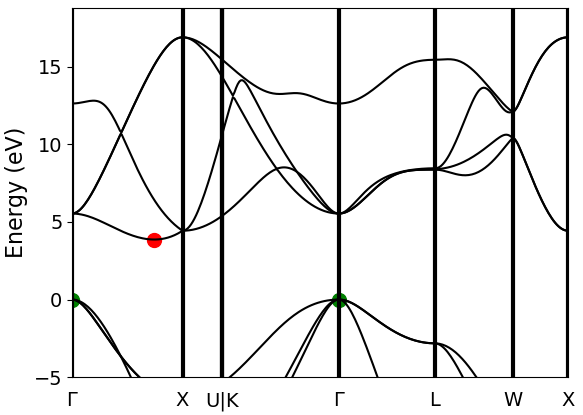
\includegraphics[width=0.5\textwidth]{figures/lab_excited_band_si}
	\caption{Band structure calculation of C-diamond performed at DFT-LDA level. Conduction band minimum (CBM) are shown with red points, and the valence band maximum(VBM)  are shown with the green points both at $\Gamma$.  DFT-LDA calculations suggest that the material has an indirect band gap from $\Gamma\rightarrow{\Delta}$. However, $\Gamma\rightarrow{\Gamma}$ transition can also be investigated for more complete check. }
	\label{fig:lab_ex_bands}
\end{figure}

\subsection{DFT band structure calculation along high symmetry paths}
After the high-symmetry kpoints are identified, one can perform band structure calculations in DFT. 
For an insulating structure, DFT can provide VBM and CBM wavevectors which would be of interest to the DMC calculations. 
However, if available, CBM and VBM from DFT would need to be compared to the experiments.  
Basically,  \texttt{band.py} will:
\begin{enumerate}
	\item Perform an SCF calculation in QE using a high density reciprocal grid.
	\item Identifies the high-symmetry k-points on the iBZ and provides a k-path.
	\item Perform a 'band' calculation in QE explicitly writing all the k-points on the path. (Make sure to add extra unoccupied bands)
	\item Plot the band structure curves and the location of VBM/CBM if available.
\end{enumerate}
In Fig. \ref{fig:lab_ex_bands}, C-diamond is shown to have an indirect band gap between the red and green dots (CBM and VBM respectively). 
VBM is located at $\Gamma$. CBM is not located on a high symmetry k-point in this case. 
Therefore, we can use the symbol $\Delta$ to denote the CBM wavevector in the rest of this document. 
In \texttt{band.py} script, once the band structure calculation is finished, you can use the following lines to get the exact location of VBM and CBM using:
\begin{lstlisting}
p = band.load_analyzer_image()
print "VBM:\n{0}".format(p.bands.vbm)
print "CBM:\n{0}".format(p.bands.cbm)
\end{lstlisting}
Output must be the following:
\begin{shade}
VBM:
  band_number     = 3
  energy          = 13.2874
  index           = 0
  kpoint_2pi_alat = [0. 0. 0.]
  kpoint_rel      = [0. 0. 0.]
  pol             = up

CBM:
  band_number     = 4
  energy          = 17.1545
  index           = 51
  kpoint_2pi_alat = [0.        0.1095605 0.       ]
  kpoint_rel      = [0.3695652 0.        0.3695652]
  pol             = up
\end{shade}
\subsection{Finding a supertwist which includes all the k-points of interest}
Using the VBM and CBM wavevectors defined in the previous section, we now construct the supertwist which will hopefully contain both VBM and CBM. In Fig. \ref{fig:lab_ex_twists}, we provide a simple example using 2D rectangular lattice. 
Let us assume that we are interested in the indirect transition, $\Gamma \rightarrow X_1$. 
In Fig. \ref{fig:lab_ex_twists}a, the first BZ of the primitive cell is shown as the square centered on $\Gamma$, which is drawn using dashed lines. Due to the periodicity of the lattice, this primitive cell BZ repeats itself with spacings equal to the reciprocal lattice vectors: (2$\pi$/a, 0) and (0, 2$\pi$/a) (or (1,0) and (0,1) in crystal coordinates). 
We are interested in the  first BZ, where $X_1$ is at (0,0.5). 
In Fig. \ref{fig:lab_ex_twists}b, the first BZ of the 2x2 supercell is the smaller square, drawn using solid lines. 
In Fig. \ref{fig:lab_ex_twists}c, the BZ of the 2x2 supercell also repeats in the space, similar to Fig. \ref{fig:lab_ex_twists}a. 
Therefore, in the 2x2 supercell, $X_1$, $X_2$ and $R$ are only the periodic images of $\Gamma$.  2x2 supercell calculation can be performed in reciprocal space using [2,2] tiling matrix. 
Therefore, individual kpoints (twists) of the primitive cell are combined in the supercell calculation, which are then called as supertwists. 
In more complex primitive cell (hence BZ), more general criteria would be constructing a set of supercell reciprocal lattice vectors which contains the $\Gamma \rightarrow X_1$ (e.g. $G_1$ in Fig. \ref{fig:lab_ex_twists}) vector within their convex hull. 
Under this constraint, Wigner-Seitz radius of the simulation cell can be maximized to in an effort to reduce finite size errors. 

\begin{figure}
	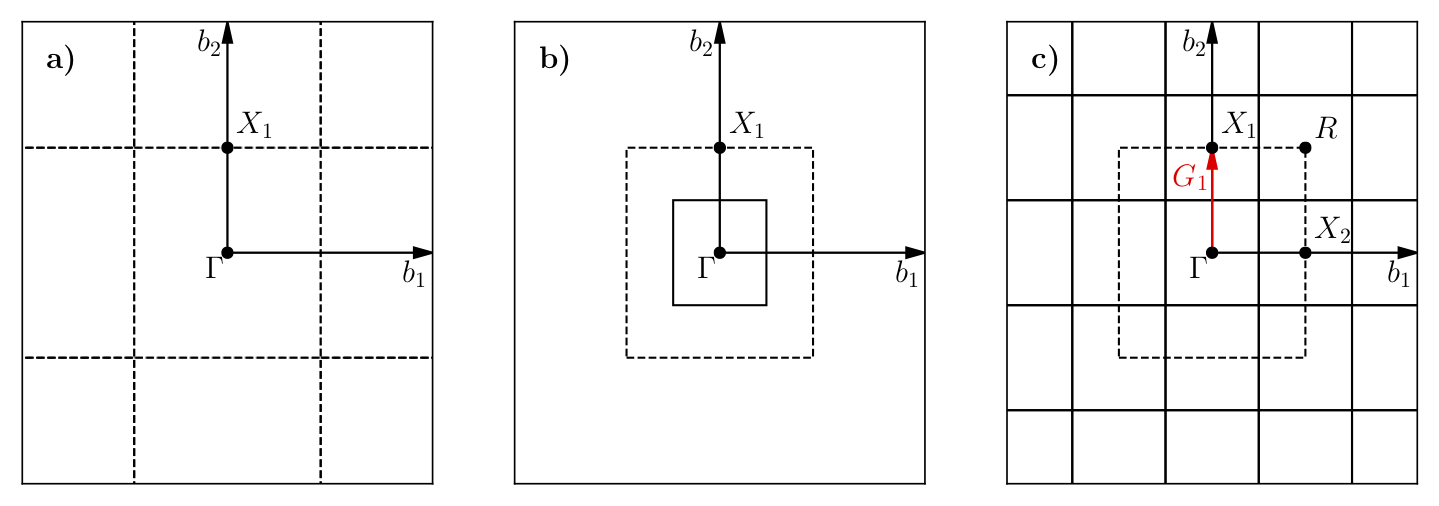
\includegraphics[width=\textwidth]{figures/lab_excited_twists}
	\caption{a) First Brillouin Zone (BZ) of the primitive cell centered on $\Gamma$. Dashed lines indicate zone boundaries. b) First BZ of the 2x2 supercell inside the first BZ of the primitive cell. First BZ boundaries of the supercell are shown using solid lines. c) Periodic translations of the first BZ of the supercell showing that $\Gamma$ and $X_1$ are periodic images of each other given the supercell BZ. }
	\label{fig:lab_ex_twists}
\end{figure}

For the case of the indirect band gap in Diamond, one may need to deal with using several approximations to generate a supertwist which corresponds to a reasonable simulation cell. 
$\Delta$ in Diamond band gap is at \texttt{[0.3695653, 0., 0.3695653]}. 
In your calculations, the $\Delta$ wavevector and the eigenvalues you find can be slightly different in value. 
Closest simple fraction to this number with the smallest denominator is 1/3. If we use $\Delta'=[1/3, 0., 1/3]$, we could use 3x1x3 supercell as the simple choice and include both $\Delta'$ and $\Gamma$ in the same supertwist exactly. 
Near  $\Delta$, the LDA band curvature is very low and using  $\Delta'$ can indeed be a good approximation. 
We can compare the eigenvalues using their index numbers:
\begin{lstlisting}[mathescape=true]
>>> print p.bands.up[51] ## CBM, $\Delta$ ##
  eigs            = [-3.2076  4.9221  7.5433  7.5433 17.1545 19.7598 28.3242 28.3242]
  index           = 51
  kpoint_2pi_alat = [0.        0.1095605 0.       ]
  kpoint_rel      = [0.3695652 0.        0.3695652]
  occs            = [1. 1. 1. 1. 0. 0. 0. 0.]
  pol             = up
>>> print p.bands.up[46] ## $\Delta'$ ##
  eigs            = [-4.0953  6.1376  7.9247  7.9247 17.1972 20.6393 27.3653 27.3653]
  index           = 46
  kpoint_2pi_alat = [0.        0.0988193 0.       ]
  kpoint_rel      = [0.3333333 0.        0.3333333]
  occs            = [1. 1. 1. 1. 0. 0. 0. 0.]
  pol             = up
\end{lstlisting}
This shows that the eigenvalues of the first unoccupied bands in $\Delta$ and $\Delta'$ are 17.1545 and 17.1972 eV respectively, meaning that according to LDA, a correction of nearly -40 meV is obtained. 
After electronic transitions between $\Gamma$ and $\Delta'$ are studied using DMC, one can apply the LDA correction to extrapolate the results to $\Gamma$ and $\Delta$ transitions.

\subsection{Identifying the indexing of k-points of interest in the supertwist}
At this stage, we must have performed \textit{scf} calculation using a converged k-point grid and then an \textit{nscf} calculation using the supertwist kpoints given above. 
We will be using the orbitals from neutral DFT calculations, therefore we need to explicitly define the band and twist indexes of the excitations in QMCPACK (e.g. in order to define electron promotion).
In C-diamond, we can give an example by finding the band and twist indexes of $\Gamma$ and $\Delta'$. 
For this end, one can run a mock VMC calculation and read \texttt{einspline.tile\_300010003} \texttt{.spin\_0.tw\_0.g0.bandinfo.dat} file. Einspline file prints out the eigenstates information from DFT calculations. 
Therefore, we can obtain the band and the state index from this file, which can later be used to define the electron promotion. 
Below, you can see an explanation of how the band and twist indexes are defined using a portion of the \texttt{einspline.tile\_300010003.spin\_0.tw\_0.g0.bandinfo.dat} file. 
Spin\_0 in the file name suggests that we are reading the spin up eigenstates. Band, state, twistindex and bandindex numbers all start from zero. We know that we have 72 electrons in the simulation cell, where 36 of them are spin-up polarized. 
Since state number starts from 0, state number 35 must be occupied while state 36 should be unoccupied. 
States 35 and 36 have the same reciprocal crystal coordinates (K1,K2,K3) as $\Gamma$ and $\Delta'$, respectively. 
Therefore, one should promote an electron from state number 35 to 36 to study the indirect band gap here. 
\begin{shade}
#  Band State TwistIndex BandIndex Energy Kx Ky Kz K1 K2 K3 KmK
33 33 0  1     0.488302  0.0000  0.0000  0.0000 -0.0000 -0.0000 -0.0000      1
34 34 0  2     0.488302  0.0000  0.0000  0.0000 -0.0000 -0.0000 -0.0000      1
35 35 0  3     0.488302  0.0000  0.0000  0.0000 -0.0000 -0.0000 -0.0000      1
36 36 4  4     0.631985  0.0000 -0.6209  0.0000 -0.3333 -0.0000 -0.3333      1
37 37 8  4     0.631985  0.0000 -1.2418  0.0000 -0.6667 -0.0000 -0.6667      1
38 38 0  4     0.691907  0.0000  0.0000  0.0000 -0.0000 -0.0000 -0.0000      1
\end{shade}
However, one should always check whether this is really what we want. 
It can be seen  that band \# 33, 34 and 35 are degenerate (energy eigenvalues are listed in the 5th column), but also they have the same reciprocal coordinates in (K1,K2,K3). 
This is actually expected as one can see from Fig. \ref{fig:lab_ex_bands}, in the band diagram the band structure is threefold degenerate at $\Gamma$.  
Here, we can choose the state with the largest band index: (0,3). 
Following the (twistindex, bandindex) notation, we can say that $\Gamma$ to $\Delta'$ transition can be defined as from (0,3) to (4,4). 

Alternatively, one can also read the band and twist indexes using PwscfAnalyzer and determine the band/twist indexes on the go:
\begin{lstlisting}
p = nscf.load_analyzer_image()
print 'band information'
print p.bands.up
print 'twist 0 k-point:',p.bands.up[0].kpoint_rel
print 'twist 4 k-point:',p.bands.up[4].kpoint_rel
print 'twist 0 band 3 eigenvalue:',p.bands.up[0].eigs[3]
print 'twist 4 band 4 eigenvalue:',p.bands.up[4].eigs[4]
\end{lstlisting}
Giving output:
\begin{shade}
  0
    eigs            = [-8.0883 13.2874 13.2874 13.2874 18.8277 18.8277 18.8277 25.9151]
    index           = 0
    kpoint_2pi_alat = [0. 0. 0.]
    kpoint_rel      = [0. 0. 0.]
    occs            = [1. 1. 1. 1. 0. 0. 0. 0.]
    pol             = up
  1
    eigs            = [-5.0893  3.8761 10.9518 10.9518 21.5031 21.5031 21.5361 28.2574]
    index           = 1
    kpoint_2pi_alat = [-0.0494096  0.0494096  0.0494096]
    kpoint_rel      = [0.3333333 0.        0.       ]
    occs            = [1. 1. 1. 1. 0. 0. 0. 0.]
    pol             = up
  2
    eigs            = [-5.0893  3.8761 10.9518 10.9518 21.5031 21.5031 21.5361 28.2574]
    index           = 2
    kpoint_2pi_alat = [-0.0988193  0.0988193  0.0988193]
    kpoint_rel      = [0.6666667 0.        0.       ]
    occs            = [1. 1. 1. 1. 0. 0. 0. 0.]
    pol             = up
  3
    eigs            = [-5.0893  3.8761 10.9518 10.9518 21.5031 21.5031 21.5361 28.2574]
    index           = 3
    kpoint_2pi_alat = [ 0.0494096  0.0494096 -0.0494096]
    kpoint_rel      = [0.        0.        0.3333333]
    occs            = [1. 1. 1. 1. 0. 0. 0. 0.]
    pol             = up
  4
    eigs            = [-4.0954  6.1375  7.9247  7.9247 17.1972 20.6393 27.3652 27.3652]
    index           = 4
    kpoint_2pi_alat = [0.        0.0988193 0.       ]
    kpoint_rel      = [0.3333333 0.        0.3333333]
    occs            = [1. 1. 1. 1. 0. 0. 0. 0.]
    pol             = up
  5
    eigs            = [-0.6681  2.3791  3.7836  8.5596 19.3423 26.2181 26.6666 28.0506]
    index           = 5
    kpoint_2pi_alat = [-0.0494096  0.1482289  0.0494096]
    kpoint_rel      = [0.6666667 0.        0.3333333]
    occs            = [1. 1. 1. 1. 0. 0. 0. 0.]
    pol             = up
  6
    eigs            = [-5.0893  3.8761 10.9518 10.9518 21.5031 21.5031 21.5361 28.2574]
    index           = 6
    kpoint_2pi_alat = [ 0.0988193  0.0988193 -0.0988193]
    kpoint_rel      = [0.        0.        0.6666667]
    occs            = [1. 1. 1. 1. 0. 0. 0. 0.]
    pol             = up
  7
    eigs            = [-0.6681  2.3791  3.7836  8.5596 19.3423 26.2181 26.6666 28.0506]
    index           = 7
    kpoint_2pi_alat = [ 0.0494096  0.1482289 -0.0494096]
    kpoint_rel      = [0.3333333 0.        0.6666667]
    occs            = [1. 1. 1. 1. 0. 0. 0. 0.]
    pol             = up
  8
    eigs            = [-4.0954  6.1375  7.9247  7.9247 17.1972 20.6393 27.3652 27.3652]
    index           = 8
    kpoint_2pi_alat = [0.        0.1976385 0.       ]
    kpoint_rel      = [0.6666667 0.        0.6666667]
    occs            = [1. 1. 1. 1. 0. 0. 0. 0.]
    pol             = up

twist 0 k-point: [0. 0. 0.]
twist 4 k-point: [0.3333333 0.        0.3333333]
twist 0 band 3 eigenvalue: 13.2874
twist 4 band 4 eigenvalue: 17.1972
\end{shade}

\section{Quasiparticle (electronic) gap calculations}\label{sec:lab_ex_qp}
In quasiparticle calculations, it is essential to work with reasonably large sized supercells in order to avoid spurious "1/N effects". 
Since quasiparticle calculations involve charged cells, large simulation cells ensure that the extra charge is diluted over the simulation cell. Coulombic interactions are conditionally convergent for neutral periodic systems, but they are divergent for the charged systems. 
A typical workflow for a quasiparticle calculation includes:
\begin{enumerate}
	\item SCF calculation in a neutral charged cell with QE using a high-density reciprocal grid.
	\item Choose a tiling matrix which will at least approximately include VBM and CBM k-points. 
	\item 'nscf'/'p2q' calculations using the tiling matrix 
	\item VMC/DMC calculations for the neutral, positively and negatively charged cells in QMCPACK
	\item Check the convergence of the quasiparticle gap with respect to the simulation cell size
\end{enumerate}
\begin{lstlisting}
<particleset name="e" random="yes">
  <group name="u" size="36" mass="1.0"> ##Change size to 35
    <parameter name="charge"              >    -1                    </parameter>
    <parameter name="mass"                >    1.0                   </parameter>
  </group>
...
...
<determinantset>
  <slaterdeterminant>
    <determinant id="updet" group="u" sposet="spo_u" size="36"> ##Change size to 35
      <occupation mode="ground" spindataset="0"/>	
    </determinant>
    <determinant id="downdet" group="d" sposet="spo_d" size="36">
      <occupation mode="ground" spindataset="1"/>	
    </determinant>
  </slaterdeterminant>
</determinantset>
\end{lstlisting}
Going back to equation \ref{eq:qp}, one can see that it is essential to include VBM and CBM wavevectors in the same twist for quasiparticle calculations as well. 
Therefore, the added electron will sit at CBM while the subtracted electron will be removed from VBM. 
However, for the charged cell calculations, one may need to make changes in the input files for the fourth step.  Alternatively, in \texttt{quasiparticle.py} file the changes in the qmc input are shown for negatively charged system:
\begin{lstlisting}
qmc.input.simulation.qmcsystem.particlesets.e.groups.u.size +=1
qmc.input.simulation.qmcsystem.wavefunction.determinantset.slaterdeterminant.determinants.updet.size += 1
\end{lstlisting}
Here, the number of up electrons are increased by one (negatively charged system), and QMCPACK is instructed to read more one orbital in the up channel from the .h5 file. 

QE uses symmetry in order to reduce the number of k-points required for the calculation. 
Therefore, all symmetry tags in QE (\texttt{nosym}, \texttt{noinv} and \texttt{nosym\_evc}) must be set to false. 
An easy way to check whether this is the case is to see that all KmK values \texttt{einspline} files are equal to 1. 
Above, the input for the neutral cell is given, while the changes are denoted as comments for the positively charged cell. 
Notice that, we have used \texttt{det\_format      = \char`\'old\char`\'} in the \texttt{vmc\_+/-e.py} files.
\section{Optical gap calculations}
Routines for the optical gap calculations are very similar to the quasiparticle gap calculations. 
The first three items in the quasiparticle band gap calculations can be reused for the optical gap calculations. 
However, at the VMC/DMC level, one should explicitly state the electronic transitions that are performed. 
Therefore, compared to the quasiparticle calculations, only the item number 4 is different for optical gap calculations. 
Here, the modified input file is given for the $\Gamma\rightarrow\Delta'$ transition, which can be compared to the ground state input file in the previous section. 
\begin{lstlisting}
<determinantset>
  <slaterdeterminant>
    <determinant id="updet" group="u" sposet="spo_u" size="36">
      <occupation mode="excited" spindataset="0" format="band" pairs="1" >
        0 3 4 4
      </occupation>
    </determinant>
    <determinant id="downdet" group="d" sposet="spo_d" size="36">
      <occupation mode="ground" spindataset="1"/>	
    </determinant>
  </slaterdeterminant>
</determinantset>
\end{lstlisting}
We have used the (twistindex, bandindex) notation in the annihilaion/creation order for the up spin electrons.
After resubmitting the batch job, in the output, you should be able to see the following lines in the \texttt{vmc.out} file:
\begin{lstlisting}
Sorting the bands now:
  Occupying bands based on (ti,bi) data.
removing orbital 35
adding orbital 36
We will read 36 distinct orbitals.
There are 0 core states and 36 valence states.
\end{lstlisting}
And the \texttt{einspline.tile\_300010003.spin\_0.tw\_0.g0.bandinfo.dat} file must be changed in the following way: 
\begin{lstlisting}
#  Band State TwistIndex BandIndex Energy Kx Ky Kz K1 K2 K3 KmK
33 33 0	1 0.499956	0.0000  0.0000 0.0000  0.0000 0.0000  0.0000 1
34 34 0	2 0.500126	0.0000  0.0000 0.0000  0.0000 0.0000  0.0000 1
35 35 4	4 0.637231	0.0000 -0.6209 0.0000 -0.3333 0.0000 -0.3333 1
36 36 0	3 0.502916	0.0000  0.0000 0.0000  0.0000 0.0000  0.0000 1
37 37 8	4 0.637231	0.0000 -1.2418 0.0000 -0.6667 0.0000 -0.6667 1
38 38 0	4 0.699993	0.0000  0.0000 0.0000  0.0000 0.0000  0.0000 1
\end{lstlisting}
Alternatively, one can define the excitations within Nexus as shown in \texttt{optical.py} file:
\begin{lstlisting}
qmc = generate_qmcpack(
    ...
    excitation = ['up', '0 3 4 4'], # (ti, bi) notation
    #excitation = ['up', '-35 + 36'], # Orbital (state) index notation
    ...
    )
\end{lstlisting}



%% \renewcommand{\chaptername}{}
%% \renewcommand{\thechapter}{}
\chapter*{References}
\addcontentsline{toc}{chapter}{References}
\begin{btSect}{bibliography}
\btPrintCited
\end{btSect}
\end{btUnit}
\end{document}

%%% Local Variables:
%%% mode: latex
%%% TeX-master: t
%%% End:
